\documentclass[10pt,final]{IEEEtran}
\usepackage{amsmath,graphicx}
\usepackage{amsmath}
\usepackage{graphicx}
\usepackage{float}
\usepackage{multirow}
%\usepackage{refcheck}
%\usepackage{spconf,amsmath,graphicx}
\usepackage{graphicx}
\usepackage{epsfig}
\usepackage{amsmath}
\usepackage{amssymb,algorithmic}
\usepackage{subfigure}
\usepackage{wrapfig}
\usepackage{times,color}
\usepackage{cite,footnote,xspace,syntonly,theorem,algorithm,algorithmic,amsthm}
\usepackage{enumerate}
\input{mysymbol.sty}
% \newenvironment{proof}{\paragraph{Proof:}}{\hfill$\square$}

% \newtheorem{theorem}{Theorem}[section]
% \newtheorem{lemma}[theorem]{Lemma}

% *** GRAPHICS RELATED PACKAGES ***
%
\ifCLASSINFOpdf
  % \usepackage[pdftex]{graphicx}
  % declare the path(s) where your graphic files are
  % \graphicspath{{../pdf/}{../jpeg/}}
  % and their extensions so you won't have to specify these with
  % every instance of \includegraphics
  % \DeclareGraphicsExtensions{.pdf,.jpeg,.png}
\else
  % or other class option (dvipsone, dvipdf, if not using dvips). graphicx
  % will default to the driver specified in the system graphics.cfg if no
  % driver is specified.
  % \usepackage[dvips]{graphicx}
  % declare the path(s) where your graphic files are
  % \graphicspath{{../eps/}}
  % and their extensions so you won't have to specify these with
  % every instance of \includegraphics
  % \DeclareGraphicsExtensions{.eps}
\fi

\long\def\symbolfootnote[#1]#2{\begingroup
\def\thefootnote{\fnsymbol{footnote}}
\footnote[#1]{#2}\endgroup} \psfull

\hyphenation{op-tical net-works semi-conduc-tor}


\begin{document}
%
% paper title
% Titles are generally capitalized except for words such as a, an, and, as,
% at, but, by, for, in, nor, of, on, or, the, to and up, which are usually
% not capitalized unless they are the first or last word of the title.
% Linebreaks \\ can be used within to get better formatting as desired.
% Do not put math or special symbols in the title.
\title{Online Kernel-Based Clustering}
%
%
% author names and IEEE memberships
% note positions of commas and nonbreaking spaces ( ~ ) LaTeX will not break
% a structure at a ~ so this keeps an author's name from being broken across
% two lines.
% use \thanks{} to gain access to the first footnote area
% a separate \thanks must be used for each paragraph as LaTeX2e's \thanks
% was not built to handle multiple paragraphs
%

\author{{Abrar Alam, Akshay Malhotra, \emph{IEEE Member} and Ioannis D. Schizas}, \emph{IEEE Member}}




% The paper headers


% note the % following the last \IEEEmembership and also \thanks -
% these prevent an unwanted space from occurring between the last author name
% and the end of the author line. i.e., if you had this:
%
% \author{....lastname \thanks{...} \thanks{...} }
%                     ^------------^------------^----Do not want these spaces!
%
% a space would be appended to the last name and could cause every name on that
% line to be shifted left slightly. This is one of those "LaTeX things". For
% instance, "\textbf{A} \textbf{B}" will typeset as "A B" not "AB". To get
% "AB" then you have to do: "\textbf{A}\textbf{B}"
% \thanks is no different in this regard, so shield the last } of each \thanks
% that ends a line with a % and do not let a space in before the next \thanks.
% Spaces after \IEEEmembership other than the last one are OK (and needed) as
% you are supposed to have spaces between the names. For what it is worth,
% this is a minor point as most people would not even notice if the said evil
% space somehow managed to creep in.




% The only time the second header will appear is for the odd numbered pages
% after the title page when using the twoside option.
%
% *** Note that you probably will NOT want to include the author's ***
% *** name in the headers of peer review papers.                   ***
% You can use \ifCLASSOPTIONpeerreview for conditional compilation here if
% you desire.




% If you want to put a publisher's ID mark on the page you can do it like
% this:
%\IEEEpubid{0000--0000/00\$00.00~\copyright~2015 IEEE}
% Remember, if you use this you must call \IEEEpubidadjcol in the second
% column for its text to clear the IEEEpubid mark.



% use for special paper notices
%\IEEEspecialpapernotice{(Invited Paper)}

\markboth{}%
{Alam: Title}


% make the title area
\maketitle\maketitle


\symbolfootnote[0]{$*$ The work in this paper was supported by ARO grant W911NF-21-1-0231. The authors are with the Dept. of
Electrical Engineering, University of Texas at Arlington, 416
Yates Street, Arlington, TX 76010. Tel/fax: (817)
272-3467/272-2253; Email:
\texttt{abrarul.alam@mavs.uta.edu,schizas@uta.edu}.} \vspace{-0.4cm}

% As a general rule, do not put math, special symbols or citations
% in the abstract or keywords.
\begin{abstract}
A novel online joint kernel learning and clustering (OKC) framework is derived which is capable of determining time-varying clustering configurations without the need for training data. To facilitate clustering via sparse kernel factorization, a novel time-dependent metric is devised to quantify closeness of candidate kernel similarity matrices to a block diagonal structure. The later task is performed online as newly acquired data are processed making it appropriate for nonstationary settings.  The necessary minimization to carry out kernel learning and clustering is performed via an effective interplay among block coordinate descent, difference of convex functions minimization and projected subgradient descent which results an online iterative algorithm that updates online the kernel covariance matrix, as well as the associated clustering configuration. The resulting recursive kernel updates are proved to converge to  a bounded limit. Detailed numerical examples utilizing both synthetic and real data show the superior clustering accuracy achieved by the novel approach over existing alternatives while requiring considerably less running time.
\end{abstract}

% Note that keywords are not normally used for peerreview papers.
\begin{IEEEkeywords}
Kernel learning, Online Algorithms, Clustering, Optimization
\end{IEEEkeywords}






% For peer review papers, you can put extra information on the cover
% page as needed:
% \ifCLASSOPTIONpeerreview
% \begin{center} \bfseries EDICS Category: 3-BBND \end{center}
% \fi
%
% For peerreview papers, this IEEEtran command inserts a page break and
% creates the second title. It will be ignored for other modes.
\IEEEpeerreviewmaketitle



\section{Introduction}
%\IEEEPARstart{D}e
%\textbf{Notation:} $^{\dag}$ denotes pseudoinverse, $[\bbM]_{q:}$ %denotes the $qth$ row of matrix $\bbM$, $[\bbM]_{:q}$ denotes the %$qth$ column of matrix $\bbM$, $\bbI_{D}$ corresponds to an identity %matrix of size $D\times D$, $\textrm{vec}(\bbM)$ corresponds to a %column vector obtained after stacking the columns of matrix $\bbM$ %moving from left to right. $\otimes$ denotes the Kronecker product %operator, $\|\cdot\|_F$ indicates the Frobenius norm. %$\textrm{diag}(\bbv)$ indicates a diagonal matrix whose diagonal %entries are the elements of vector $\bbv$, and $\mathbf{1}_n$ %corresponds to the all-ones $n\times 1$ vector and $\mathbb{E}[\cdot]$ %is the expectation operator.
The acquisition of ever increasing amounts of sensor measurements has created a need to categorize the data via unsupervised clustering techniques {{\cite{sensors}}}. Multiple sensors measuring a physical quantity in a localized environment, generate data that tend to be correlated, especially if the sensor measurements are influenced by the same  underlying source or phenomenon. Such correlations among the acquired data vectors can be utilized to achieve data clustering goals since signals/measurements containing information about the same source tend to be strongly correlated. Several sensing applications varying from human activity detection and recognition \cite{Human_Activity} to hyper-spectral imaging \cite{Hyperspectral_Images} generate data that need to be clustered according to their information content and the phenomena they observe.

Many clustering algorithms have been developed dealing with linear correlations and utilizing traditional covariance/correlation matrices as a similarity metric to achieve data clustering.  Towards this end, canonical correlation analysis (CCA) based clustering methods  suitable for linear data models were proposed in \cite{CCA}. The correlation-based clustering schemes were formulated as a matrix factorization problem in \cite{Distributed Informative-Sensor} which was solved with norm-1 sparsity formulations. An augmented Lagrangian approach towards solving an orthogonal NMF problem was presented in \cite{Neurocomputing}. A comprehensive review of different NMF algorithms can be found in \cite{NNMF Comprehensive}.

To address non-linear settings  where linear data correlations are ineffective in idenifying the underlying data clustering, kernel methods have been proposed.  These methods leverage kernel-based correlation matrices that can unveil linear correlations in higher-dimensional spaces. Kernel target alignment \cite{Kernel_Target} is one such popular supervised approach wherein the suitable kernel matrices are identified by finding the alignment or the normalized inner product between the kernel correlation matrices and the correlation of the class labels. 
% A combination of Perceptron and Hedge based algorithms has been used towards kernel learning in \cite{Online Multiple Kernel Learning}. These approaches  are supervised or semi-supervised in nature.

Recently unsupervised approaches have been proposed to jointly construct a proper kernel similarity matrix while performing data clustering. The unsupervised approach in \cite{SPMKC} relies on building proper graph similarity matrices to model correlations among the data vectors via an affine weight strategy while preserving the data structure via proper constraints. Further, relying on tensor factorization the method in \cite{tkmgc} offers a more computationally expensive option while improving clustering in a variety of different datasets. Another unsupervised joint kernel learning and clustering approach in \cite{DCA} utilizes a sparsity regularized nonnegative matrix factorization along with eigenvalue maximization to find proper kernel covariance matrices that facilitate data clustering.

The aforementioned approaches are unsupervised and do not require training data, nonetheless these methods are developed for time-invariant datasets in which the clustering configuration is stationary. 
% Prior to discussing the details of the novel algorithm presented in this paper, it is important to shed some insight on the motivation that led to this work. 
Several online learning have also been developed
%has been a widely studied research topic in machine learning as it was designed 
with the intention of learning and evolving the machine learning models  sequentially, as new information becomes available. In \cite{Online MKL,Online Multiple Kernel Learning} an online learning setup for multiple kernel learning has been introduced. The method combines the Perceptron and Hedge based algorithms  towards kernel learning. In \cite{Semi-supervised} a semi-supervised approach which relies on online kernel learning to accurately classify web pages to facilitate enhanced searches on the internet was proposed.

Large scale online clustering was investigated in \cite{LSOKL} where the motivation was to make online learning algorithms highly scalable and efficient by minimizing high re-training algorithms in stationary settings. This is particularly important for processing enormous datasets that arrive sequentially and evolve dynamically as well as rapidly. Moreover, \cite{MKL} focuses on decreasing the generalization error by addressing the fact that more features should lead to improved performance. The intention here was to create a novel framework that would perform feature selection while training and hence, an algorithm was developed that would implement a new optimization technique to solve the $l_p$-multiple kernel learning problem with a guaranteed convergence rate to the optimal solution. Finally, \cite{OEML}, \cite{OMKLGSF}, and \cite{Random OMKL} have also discussed the importance of multiple kernel learning and how it can be combined with online learning to facilitate scalable learning on large volumes of datasets. 
Although these methods have addressed the problem of kernel learning in large data settings by enabling sequential processing and ensuring scalability. Existing online kernel learning methods are largely supervised or semi-supervised. In large scale online settings the labels for data  vectors are not easily available. Specially in unsupervised settings, like the ones considered in this work, the labels for the data vectors are assumed to be unknown. This motivates the need for a \textit{truely unsupervised} framework capable of doing joint kernel learning and data clustering in online settings.   
% Thus, it can be inferred that the motivation for the development of this algorithm can be attributed towards a more scalable processing of large volumes of sequential sensor data by selecting the appropriate task-specific kernels from a prescribed dictionary of kernels.

In the present work we generalize the approach in \cite{DCA} to address non-stationary settings in which there is a constant flow of data contrary to \cite{SPMKC,tkmgc,DCA} where the dataset is fixed. A novel framework in derived here relying on exponential weighing to give more emphasis to recently acquired data vectors while gradually forgetting the past. An time-varying  metric is proposed to 
facilitate the online construction of block diagonal kernel similarity matrices that facilitate data clustering in time-varying cluster configurations. An interplay of block coordinate descent, difference of convex formulation and subgradient descent \cite{Convex Analysis,subgradient methods,Convex} is employed to devise an online joint kernel learning and clustering method. A convergent iterative algorithm is obtained that achieves competitive clustering accuracy with respect to existing alternatives \cite{SPMKC,tkmgc} while requiring considerably less running time.





%Several kernel-based clustering methods have been explored in the past. [1] centers its efforts around hyper-spectral images which consist of a collection of images taken across hundreds of different spectral bands. These images were particularly helpful as their spectral reflectance values were indicative of the variety of materials/objects present. In this work, an algorithm was built that combined norm-1 regularization in a canonical correlations framework and statistical correlations between mixed pixels to estimate the contribution of endmembers within the mixed pixels of the images. The combination of techniques applied in the algorithm allowed it to be robust and effective under highly non-linear data mixtures, even when they are corrupted by unresponsive pixels. On the contrary, two correlation-based analysis procedures were introduced in [2] that focused on a human activity detection dataset and eliminated the requirement for any prior segmentation or feature extraction before performing classification. The advantage of this integrated correlation-based analysis technique is that it can be applied directly on the dataset, whereas other techniques first relied on the extraction of target features, and then performed the intended clustering tasks. Moreover in [3], a mixed integer linear programming (MILP) was employed to address the issues of non-convex matrix factorization based clustering.

%The increment in the number of clustering applications in next generation wireless networks led to the development of multiple kernel graph-based clustering (MKGC) which overcame the challenges of single kernel selection methods and helped to facilitate large amounts of non-linear and unlabeled data. However, this clustering method came with its own set of issue and in order to combat them, TKMGC [4] was created which combined non-negative matrix factorization (NMF) and graph learning together in a kernel space for learning multiple candidate affinity graphs. Another method described in [6] integrates PCA and moving-averaging (MA) filtering to ensure an enhanced clustering approach that can group sensor reading based on their information content. It also employs a norm-1 regularized canonical correlation analysis technique which further allows the algorithm to extract correlated sensor measurements and group them in clusters. Nevertheless, there is one thing that was not explored by any of the methods described above and that is real-time, online kernel-based clustering proposed in this paper.
The contributions of our novel work are: 
\begin{enumerate}[(i).]
    \item Derivation of a time-varying metric to quantify closeness of candidate kernel mappings to a block diagonal structure that facilitates joint  kernel learning and factorization-based clustering. 
    \item A novel minimization formulation to enable clustering in nonstationary settings where contrary to existing works \cite{SPMKC,tkmgc,DCA} the data clusters are time-dependent. 
    \item A novel interplay of block coordinate descent, difference of convex programming and projected subgradient descent techniques are utilized to construct an online algorithm that processes data on-the-fly and provides refined cluster membership. 
    \item Convergence of the novel online approach is established showing that the kernel updates move closer to a block diagonal structure.  
    \item Extensive numerical tests demonstrate the clustering accuracy advantage of the novel framework over existing alternatives as well as reduced running time required.
\end{enumerate}

The reminder of the paper is structured as follows: (i) Problem Statement and preliminary concepts are provided in Sec. II while explaining the idea of clustering via a proper block diagonal kernel covariance matrix construction; (ii) In Sec. III the novel time-varying metric quantifying the quality of a block diagonal kernel covariance matrix is derived. Further, the novel online kernel clustering (OKC) algorithm is constructed via a novel collaboration between block coordinate descent, difference of convex approach and projected subgradient descent while convergence is established; (iii) Extensive numerical tests are performed in Sec. IV for the novel algorithm along with state-of-the-art clustering methods using synthetic and real datasets and evaluating accuracy, the normalized mutual information (NMI) and purity. 


\section{Problem Statement}\label{sec:problem_statement}
Consider a set of $P$ data measurements acquired at time instants $\tau=0,1,\ldots$, namely $\{x_{i}(\tau)\}_{i=1}^{P}$. Each of the $P$ data vectors are assumed to contain information from exactly one source (or class) from a total population of $Q$ sources (or classes). Thus, the set of $P$ data measurements can be split in $Q$ subgroups (or clusters) where the measurements within each subgroup are influenced by the same source signal. The cluster configuration corresponding to the given set of data vectors, $\{x_{i}(\tau)\}_{i=1}^{P}$, is unknown, and the primary objective is to  cluster the $P$ data vectors into $Q$ subgroups using only the available data measurements. The cluster configuration of the acquired data can also be time-varying. This is a major difference with our work in \cite{DCA}, as well as the majority of unsupervised clustering methods \cite{tkmgc,SPMKC} in which case the clustering configuration is fixed. To this end, there is a  need to develop an unsupervised clustering framework that can process data online and is capable of tracking the time-varying data clustering configurations.

Measurement $x_i(\tau)$ acquired at time instant $\tau$ can modeled as,  
%%
\begin{align}\label{eq:linear_relation}
x_{i}(\tau) =\textstyle \sum_{q=1}^{Q}c_q^i \xi_q(s_q(\tau))+w_i(\tau),
\end{align}
%%
where $\xi_q(\cdot)$ is a nonlinear, not necessarily known, mapping which dictates how $x_i(\tau)$ is affected by  the $q$th source signal $s_q(\tau)$ at time $\tau$, and $c_q^i$ indicates the membership of the $i$-th sensor towards the $q$th class (or $q$th source). Further, we assume a non-overlapping observation-source setting, in which for a given measurement $x_i(\tau)$, the set of  membership variables given by $\{c_q^i | q \in \{1, ..., Q\}~\}$, contains only one non-zero variable while the source signals $s_q(\tau)$ are uncorrelated. The objective here is to identify how the  $P$ data measurements can be clustered in $Q$ subgroups at time instant $\tau$, such that data measurements observing the same source are clustered together.


\subsection{Clustering via Kernel Covariance Factorization}\label{sec:Fact_Kernel}
 The data covariance matrix within time horizon $[0,t-1]$ can be found as
%%%%%%%%%
\begin{equation}\label{eq:linear_correlation}
\mathbf{K}_t[i,j] = {t}^{-1}\textstyle\textstyle\sum_{\tau= 0}^{t-1}{(x_i(\tau) - \bar{x}_i(t))(x_j(\tau)-\bar{x}_j(t))} ,
\end{equation}
where $\bar{x}_i(t) = t^{-1} \sum_{\tau=0}^{t-1} x_i(\tau)$ is the sample-average of measurements $x_i(\tau)$ for $\tau\in[0,t-1]$ while $i,j=1,\ldots,P$.

When the unknown mappings are linear, i.e., $\xi_q(s_q)=b_q\cdot s_q$ where $b_q$ is a constant, the covariance matrix in \eqref{eq:linear_correlation} can be rewritten as 
%%
\begin{equation}\label{eq:linear_corr_fact}
\mathbf{K}_t= \mathbb{E}[t^{-1}\bbX_t\bbX_t^T]=\mathbf{F}_t\mathbf{D_s(t)}\mathbf{F}_t^T
\end{equation}
%%
where $\mathbb{E}[\cdot]$ denotes the ensemble mean and $\bbX_t:=[\bbx_0\;\bbx_1\;\ldots\;\bbx_{t-1}]\in\mathbb{R}^{P\times t}$ with $\bbx_{\tau}=[x_1(\tau),x_2(\tau),\ldots,x_P(\tau)]^T$ for $\tau=0,\ldots,t-1$. The diagonal matrix ${\mathbf{D_s}(t) \in \mathbb{R}^{Q\times Q}}$ is the source covariance matrix, assuming that sources are uncorrelated. The entries of matrix $\mathbf{F}_{t} \in \mathbb{R}^{P\times Q} $ are such that $\mathbf{F}_{t}[r,q] = \{c_{q}^{r}\cdot b_q \ne 0\}$  if the $r$th data measurement $x_r(\tau)$ acquires info about the $q$th source for $\tau\in[0,t-1]$, otherwise it is $\mathbf{F}_{t}[r,q]  = \{0\}$. Thus, factor $\bbF_{t}$ will have one nonzero entry per row while the rest of the entries will be zero. Given that $\bbD_{s}(t)$ is diagonal then the covariance matrix $\bbK_t$ will have a block diagonal structure under finite permutations of rows and equivalent column exchange operations. Further, the number of diagonal blocks is equal to the number of underlying sources $Q$.

The task of clustering the data $x_i(\tau)$ based on their source content can be achieved by determining the support of the columns of $\bbF_{t}$ denoted here  as $\textrm{supp}(\bbF_{t})$. Note that the nonzero entries in the $q$th column of $\bbF_t$ indicate which vectors observe the $q$th source for $q=1,\ldots,Q$. Since $\bbD_s(\tau)$ is a diagonal matrix, it follows that $\textrm{supp}(\bbF_t) = \textrm{supp}(\bbF_t [\bbD_s(t)]^{1/2})$. Thus, the objective is to factorize $\bbK_t$  as $\bbK_{t}=\bbW_t\bbW_t^T$  where $\bbW_t\in\mathbb{R}^{P\times Q}$, while $\bbW_t$ has one nonzero entry per row. Ideally $\textrm{supp}(\bbW_t) =
\textrm{supp}(\bbF_t)$.

In practice, the mappings $\xi_q(\cdot)$ are nonlinear. Thus, a linear covariance matrix may not be adequate in  identifying whether the data vectors are observing a common source by utilizing a block diagonal structure. To overcome this challenge, the idea used is to utilize a kernel covariance matrix
which essentially quantifies the covariance of properly transformed data vectors via a kernel mapping \cite{Online Multiple Kernel Learning,DCA}.

The unknown kernel mapping employed in the data vectors is represented as $\bbpsi : \mathbb{R}^{P} \rightarrow  \mathbb{R}^{P \times \it{D_h}}$, where $\it{D_h}$ represents the dimensionality of a higher dimensional feature space. The nonlinear mapping $\bbpsi(\cdot)$ is applied across each entry of  ${\bbx}_{\tau} \rightarrow \psi(\bbx_{\tau})$; recall that  $\bbx_{\tau}:=[x_1(\tau),x_2(\tau),\ldots,x_P(\tau)]^T$. Thus, $\bbpsi(\bbx_{n}) = [\hat\bbpsi({x_1(n)}), ...,\hat\bbpsi({x_{P}(n)})]^T$, where $\hat\bbpsi  : \mathbb{R} \rightarrow  \mathbb{R}^{\it{1\times D_h}}$. The kernel covariance matrix can then be expressed as 
%
\begin{align}
\label{eq:Kernel_Matrices1}
{\mathbf{K}}_{t}(\bbx) = t^{-1} \textstyle\sum_{\tau =0}^{t-1} \bar{\bbpsi}(\bbx_{\tau})\bar{\bbpsi}^{T}(\bbx_{\tau}).
\end{align}
%
where $\bar{\bbpsi}(\bbx_{\tau}):={\bbpsi}(\bbx_{\tau})-t^{-1}\textstyle\sum_{\tau=0}^{t-1}{\bbpsi}(\bbx_{\tau})$ corresponds to the centered kernel-mapped data. Without loss of generality we will assume that the mapped data are centered and zero-mean. 

To find a proper kernel covariance $\bbK_{t}(\bbx)$, that will boost data clustering accuracy, we will express $\bbK_{t}(\bbx)$ as a convex combination of elements from a known dictionary  of similarity kernels, namely ${\cal D}_{\tau}:=\{{\mathbf{K}}_{\tau}^b(\bbx_{\tau})\}$ where 
$b \in \{1, ..., B\}$ that can be constructed from the available data at time instant $\tau=0,1,\ldots,$. The objective will be to find a proper convex combination of kernels. The kernel matrix elements of the dictionary can be built for example using Gaussian radial basis function (RBF) kernels or polynomial kernels, i.e.,
%%
%%
\begin{align}\label{eq:RBF}
\mathbf{K}_{\tau}^{b,RBF}(r,s) &= \exp\left(-\frac{||{x}_{r}(\tau)-{x}_{s}(\tau)||^2}{2\sigma^{2}}\right),\nonumber \\
\mathbf{K}_{\tau}^{b,Poly}(r,s)&= ({x}_r(\tau)\cdot x_s(\tau))^d,
\end{align}
%%
%%
where $\sigma$ is the variance of an RBF kernel, and $d$ the degree of a polynomial kernel while $r,s=1,\ldots,P$.

Using the elements of the kernel dictionary at time instant $\tau$ the unknown kernel covariance is parameterized as follows
%%
\begin{equation}\label{eq:cvx:combination}
\bbK_{\tau}(\bbx)=\sum_{b=1}^{B} {\alpha}_b^{\tau} \mathbf{K}_{\tau}^b(\bbx_{\tau}),
\end{equation}
%%
where ${\alpha}_b \geq 0$ and $\textstyle\sum_{b=1}^{B} {\alpha}_b =1$; corresponding to a simplex convex set. These convexity constraints ensure that the weights for all the kernels sum to $1$, while the matrix in \eqref{eq:cvx:combination} is a valid positive semidefinite kernel. Since a block diagonal kernel covariance matrix, with $Q$ diagonal blocks makes it suitable for data clustering into $Q$ clusters \cite{DCA}, the goal is to select proper kernel coefficients ${\alpha}_b^{\tau}$ at every time instant $\tau$ such that kernel matrix $\bbK_{\tau}(\bbx)$ has structure as close as possible to a block diagonal matrix. Hence, facilitate clustering of the data according to the underlying source content.  

\section{Online Joint Kernel Learning and Clustering}
\label{sec:online}

In nonstationary settings, where the data clustering configuration is changing, it is pertinent to find a proper metric to effectively quantify how close kernel matrices $\bbK_{\tau}(\bbx)$ are to a block diagonal matrix with $Q$ diagonal blocks. Such a distance metric will facilitate the selection of kernel coefficients $\alpha_b^{\tau}$. We rely on exponential weighing and matrix factorization to  obtain a metric that  gradually forgets past data and weighs more recent data vectors.  Specifically, we introduce the function
%%
\begin{align}\label{eq:Nonstationary}
&B_t(\bbW,\bbY)=\textstyle\sum_{\tau=0}^{t}\beta^{t-\tau}\|\bbK_{\tau}(\bbx_{\tau})-\bbW\bbY^T\|_F^2\\
&+\nu\sum_{\ell=1}^{P}[\|\bbW_{\ell,:}\|_1-\|\bbW_{\ell,:}\|_2
+\|\bbY_{\ell,:}\|_1-\|\bbY_{\ell,:}\|_2],\nonumber
\end{align}
where $\beta\in(0,1)$ is a forgetting factor controlling the rate at which past data are `eliminated' towards determining a pertinent kernel covariance $\bbK_{t}$ parameterized according to \eqref{eq:cvx:combination}. Note that $||\cdot||_1$ and $||\cdot||_2$ are the $\ell_1$ and $\ell_2$ norms of a vector, while $\nu$ is the regularization parameter controlling the sparsity of the rows of $\bbW$ and $\bbY$. $\bbW_{i.:}$ and $\bbY_{i,:}$, refer to the $i$th row of $\bbW$ and $\bbY$ matrices, respectively. Matrices $\bbW$ and $\bbY$  are the $P\times Q$ factors that will accurately factorize a block diagonal matrix $\bbK_{\tau}(\bbx)$, in which case $\bbK_{\tau}(\bbx)=\bbW\bbY^T$, with the factors $\bbW$ and $\bbY$ ideally having one nonzero entry across each of their rows. Next, we discuss some properties of the metric $B_t(\bbW,\bbY)$ defined in \eqref{eq:Nonstationary}.
%%
\begin{lemma}\label{Lemma:Metric}
The metric $B_t(\cdot)$ is non-negative and obtains the minima of $B_t(\cdot)=0$ when $\bbK_{\tau}(\bbx_{\tau})$ has a block diagonal structure.  
\end{lemma}

%%
\begin{proof}
Refer appendix A.
\end{proof}

Thus, the metric in \eqref{eq:Nonstationary} can be utilized to guide the selection of kernel coefficients $\alpha_b^{\tau}$ that result in a kernel covariance $\bbK_{t}$ with a structure as close as possible to a block diagonal matrix.

The kernel weights should be selected such that $\bbK_{t}(\bbx)=\sum_{b=1}^{B} {\alpha}_b^t \mathbf{K}_{t}^b(\bbx_{t})$ has rank as close to Q as possible to ensure that the data is clustered in $Q$ subgroups.
To enforce such a requirement we will utilize the $Q$th largest eigenvalue of $\bbK_{t}(\bbx)$ that can  be expressed as the difference of two convex functions, i.e.,
%%
\begin{align}\label{eq:lambda_Q}
G_t(\bbalpha)&=\textstyle\sum_{q=1}^{Q}\lambda_{q}(\bbK_{t}(\bbx))-\textstyle\sum_{q=1}^{Q-1}\lambda_{q}(\bbK_{t}(\bbx)),
\end{align}
%%
where the sum of the $Q$ largest eigenvalues $\{\lambda_{q}(\bbK_{t}(\bbx))\}_{i=1}^Q$ of $\bbK_{t}(\bbx)$ is a convex function with respect to $\bbK_{t}(\bbx)$ and therefore coefficients $\bbalpha:=[\alpha_1,\ldots,\alpha_B] $\cite{Convex}.

The goal is to maximize \eqref{eq:lambda_Q} such that most of the energy is contained within the first $Q$ eigenvalues resulting in a matrix $\bbK_{t}(\bbx)$ with rank close to $Q$. Thus, the objective is to build a kernel covariance $\bbK_{t}(\bbx)$ that minimizes the metric $B_t(\cdot)$ in \eqref{eq:Nonstationary}, and maximizes $G_t(\cdot)$ in \eqref{eq:lambda_Q}. Combining the two objectives, the goal is to minimize the following cost function
%%
%%
\begin{align}\label{eq:Eq1}
&F_t(\bbW,\bbY,\bbalpha)=B_t(\bbW,\bbY)-\mu\cdot G_t(\bbalpha)\\
&=\textstyle\sum_{\tau=0}^{t}\beta^{t-\tau}\|\sum_{b=1}^{B} {\alpha}_b \mathbf{K}_{\tau}^b(\bbx_{\tau})-\bbW\bbY^T\|_F^2\nonumber\\
\hspace{-2cm}&+\nu\sum_{\ell=1}^{P}[\|\bbW_{\ell,:}\|_1-\|\bbW_{\ell,:}\|_2
+\|\bbY_{\ell,:}\|_1-\|\bbY_{\ell,:}\|_2]\nonumber\\
&+\mu(\sum_{q=1}^{Q-1}\lambda_{q}(\sum_{b=1}^{B}\alpha_j \mathbf{K}_{t}^b(\bbx_{t}))-\sum_{q=1}^{Q}\lambda_{q}(\sum_{b=1}^{B}\alpha_b\mathbf{K}_{t}^b(\bbx_{t}))))\nonumber
\end{align}
subject to the following simplex constraints for the kernel coefficients in $\bbalpha:=[\alpha_1,\alpha_2,\ldots,\alpha_B]$, i.e., 
$\sum_{b=1}^{B}\alpha_b=1$ and $\{\alpha_b\geq 0\}_{b= 1}^B$. To minimize $F_t$ at time instant $t$ we resort to block coordinate descent where $F_t$ is minimized with respect to $\bbW,\bbalpha$, while fixing $\bbY$ to its most recent update $\bbY_{t,\kappa}$ and vice versa where $\kappa$ refers to the block coordinate descent iteration index during time instant $t$.

Note that the cost function in \eqref{eq:Eq1} is nonconvex with respect to $\bbW,\bbY$ and $\bbalpha$. Interestingly, the cost function $F_t(\cdot)$   can be viewed as a difference of convex functions formulation \cite{Convex Analysis} when minimizing w.r.t  $\bbW,\bbalpha$ and fixing $\bbY=\hat{\bbY}_{t,\kappa}$. The difference of convex functions algorithm (DCA) \cite{Convex Analysis} deals with objective functions of the type $F(\bbXi)  = H(\bbXi) - J(\bbXi)$ where, $H(\bbXi)$ and $J(\bbXi)$ are convex functions. In the setting considered here: i) $\bbXi:=\{\bbW,\bbalpha\}$ corresponds to the unknown kernel factors and kernel coefficients while fixing $\bbY=\hat{\bbY}_{t,\kappa}$ to a constant value; and ii)
%%
%%
\begin{align}\label{eq:C_and_H}
   H_{W,\alpha}^{t}(\bbXi)=& \textstyle\sum_{\tau=0}^{t}\beta^{t-\tau}\|\sum_{b=1}^{B} {\alpha}_b \mathbf{K}_{\tau}^b(\bbx_{\tau})-\bbW\bbY_{t,\kappa}^T\|_F^2\nonumber\\
   &\hspace{-2cm}+\nu\sum_{\ell=1}^{P}\|\bbW_{\ell,:}\|_1+\mu[\sum_{q=1}^{Q-1}\lambda_{q}(\sum_{b=1}^{B}\alpha_b \mathbf{K}_{t}^b(\bbx_{t}))],\\
   J_{W,\alpha}^{t}(\bbXi)&= \nu\sum_{\ell=1}^{P}\|\bbW_{\ell,:}\|_2+\mu[\sum_{q=1}^{Q}\lambda_{q}(\sum_{b=1}^{B}\alpha_b \mathbf{K}_{t}^b(\bbx_{t}))],\nonumber
\end{align}
%%
%%
such that $F_t(\bbW,\bbalpha)=H_{\bbW,\bbalpha}^{t}(\bbXi)-J_{\bbW,\bbalpha}^{t}(\bbXi)$, while $H_{\bbW,\bbalpha}^{t}(\bbXi)$ and $J_{\bbW,\bbalpha}^{t}(\bbXi)$ are both convex w.r.t  $\bbXi:=\{\bbW,\bbalpha\}$ \cite{Convex}. 

Similarly when minimizing $F_t$ w.r.t  $\bbY$ while fixing $\bbW,\bbalpha$
to $\hat{\bbW}_{t,\kappa+1}$ and $\hat{\bbalpha}_{t,\kappa+1}$, then 
$\bbXi:=\bbY$ while
%%
%%
\begin{align}\label{eq:C_and_H}
   &H_Y^t(\bbXi)= \textstyle\sum_{\tau=0}^{t}\beta^{t-\tau}\|\sum_{b=1}^{B} {\alpha}_{b_{t,\kappa+1}} \mathbf{K}_{\tau}^b(\bbx_{\tau})-\bbW_{t,\kappa+1}\bbY^T\|_F^2\nonumber\\
   &+\nu\sum_{\ell=1}^{P}\|\bbY_{\ell,:}\|_1,\;\;J_Y^t(\bbXi)= \nu\cdot\sum_{\ell=1}^{P}\|\bbY_{\ell,:}\|_2,
\end{align}
%%
%%
such that $F_t(\bbY)=H_{Y}^{t}(\bbXi)-J_{Y}^{t}(\bbXi)$, while $H_{Y}^{t}(\bbXi)$ and $J_{Y}^{t}(\bbXi)$ are both convex w.r.t $\bbXi:=\bbY$ \cite{Convex}. 

When minimizing $F_t$ w.r.t  $\bbW,\bbalpha$ while fixing $\bbY=\hat{\bbY}_{t,\kappa}$, the difference of convex functions method \cite{Convex Analysis} is utilized to minimize
%%
\begin{align}\label{eq:DC_Walpha}
&(\hat{\bbW}_{t,\kappa+1},\hat{\bbalpha}_{t,\kappa+1})=\arg\min_{\bbW,\bbalpha}H_{W,\alpha}^t(\bbW,\bbalpha)-J_{W,\alpha}^t(\bbW,\bbalpha)\nonumber\\
&\textrm{s. to }\bbalpha\geq \mathbf{0}\textrm{ and }\mathbf{1}^T\bbalpha=1,
\end{align}
%%
where $\hat{\bbW}_{t,\kappa+1},\hat{\bbalpha}_{t,\kappa+1}$ corresponds to the iterates at time instant $t$, during coordinate descent iteration $\kappa+1$. 

Similarly, for minimizing $F_t$ w.r.t $\bbY$ while fixing $\bbW,\bbalpha$
to $\hat{\bbW}_{t,\kappa+1}$ and $\hat{\bbalpha}_{t,\kappa+1}$, the difference of convex functions method is again leveraged as,
%%
\begin{align}\label{eq:DC_Y}
\hat{\bbY}_{t,\kappa+1}=\arg\min_{\bbY}H_{Y}^t(\bbY)-J_{Y}^t(\bbY)
\end{align}
%%
where $\hat{\bbY}_{t,\kappa+1}$ corresponds to the $\bbY$ factor update at time instant $t$ and during coordinate descent iteration $\kappa+1$. The DC method will recursively minimize \eqref{eq:DC_Walpha} and \eqref{eq:DC_Y}  by computing an affine majorizations of the functions 
$-J_{W,\alpha}^t(\bbW,\bbalpha)$ (and $-J_{Y}^t(\bbY)$) which will be used as surrogates to relax the formulations \eqref{eq:DC_Walpha} and \eqref{eq:DC_Y} into  convex programs.

\subsection{Algorithmic Details}\label{sec:alg}
During time instant $t$ the objective is to determine the minimizers $\hat{\bbW}_t,\hat{\bbY}_t,\hat{\bbalpha}_t$ of the cost in \eqref{eq:Eq1}.
To this end, let $K$ denote the total number of block coordinate cycles we will apply to estimate $\hat{\bbW}_t,\hat{\bbY}_t,\hat{\bbalpha}_t$. First,  cost $F_t$ is minimized w.r.t  $\bbW,\bbalpha$ while fixing $\bbY=\hat{\bbY}_{t,\kappa}$
as detailed in \eqref{eq:DC_Walpha} using the difference of convex algorithm (DCA). This task involves the following two steps which are repeated until convergence (note that $\rho=0,1,2,\ldots$ refers to the DCA iteration index)

\textbf{Step a.1}: Evaluate the $P\times Q$ subgradient  matrix and $B\times 1$ subgradient vector of $J_{W,\alpha}^t(\bbW,\bbalpha)$ in \eqref{eq:DC_Walpha} w.r.t $\bbW$ and $\bbalpha$, respectively, at point $\hat{\bbW}_{t,\kappa,\rho}$ and $\hat{\bbalpha}_{t,\kappa,\rho}$, i.e.,
%%
\begin{align}\label{eq:Subgradient_Walpha}
&\bbdelta_{\bbW} J_{t,\kappa,\rho}:=\delta_{\bbW} J_{W,\alpha}^t(\hat{\bbW}_{t,\kappa,\rho},\hat{\bbalpha}_{t,\kappa,\rho}) \\
&\bbdelta_{\bbalpha} J_{t,\kappa,\rho}:=\delta_{\bbalpha} J_{W,\alpha}^t(\hat{\bbW}_{t,\kappa,\rho},\hat{\bbalpha}_{t,\kappa,\rho}) 
\end{align}
%%
with $\bbdelta_{\bbW,\bbalpha}$ indicating the subgradient operator w.r.t variables $\bbW$ and $\bbalpha$ respectively which can be found as \cite{subgradient methods} 
%%
\begin{align}\label{eq:DCA_Subgrads}
&\bbdelta_{\bbW}J_{t,\kappa,\rho}=\left[\begin{array}{c}{{||\mathbf{W}_{1},:||_2^{-1}}\cdot\bbW_{1,:}}\\
\vdots\\
{||\mathbf{W}_{P},:||_2^{-1}}\cdot\bbW_{P,:}
\end{array}\right]\\
&\bbdelta_{\bbalpha} J_{t,\kappa,\rho}=\nonumber\\
&\begin{bmatrix}
{\bbmu}_1^T\mathbf{K}_{t}^1(\bbx_{t})){\bbmu}_1+{\bbmu}_2^T\mathbf{K}_{t}^1(\bbx_{t})){\bbmu}_2+...+{\bbmu}_{Q}^T\mathbf{K}_{t}^1(\bbx_{t})){\bbmu}_{Q}\\
{\bbmu}_1^T\mathbf{K}_{t}^2(\bbx_{t})){\bbmu}_1+{\bbmu}_2^T\mathbf{K}_{t}^2(\bbx_{t})){\bbmu}_2+...+{\bbmu}_{Q}^T\mathbf{K}_{t}^2(\bbx_{t})){\bbmu}_{Q}\\
\vdots\\
{\bbmu}_1^T\mathbf{K}_{t}^B(\bbx_{t})){\bbmu}_1+{\bbmu}_2^T\mathbf{K}_{t}^B(\bbx_{t})){\bbmu}_2+...+{\bbmu}_{Q}^T\mathbf{K}_{t}^B(\bbx_{t})){\bbmu}_{Q}\nonumber,
\end{bmatrix}\nonumber
\end{align}
%%
with $\{\bbmu_q\}_{q=1}^{Q}$ corresponding to the $q$th principal eigenvector of the kernel covariance matrix $\sum_{b=1}^B\alpha_b{\bbK}_{t}^b(\bbx_{t})$.

\textbf{Step a.2:} Minimize the affine majorizer of the cost  in \eqref{eq:DC_Walpha}
%%
\begin{align}\label{eq:Majorized_F_Walpha}
&(\hat{\bbW}_{t,\kappa,\rho+1},\hat{\bbalpha}_{t,\kappa,\rho+1})  
=    \arg\min_{\bbW,\bbalpha}
\sum_{\tau=0}^{t}\beta^{t-\tau}||\sum_{b=1}^{B}\alpha_b \bbK_{\tau}^b(\bbx_{\tau})\nonumber\\
&-\bbW\hat{\bbY}_{t,\kappa}^T||_F^2
+v(\sum_{\ell=1}^{P}||{\bbW_{\ell},:}||_1)+\mu(\sum_{q=1}^{Q-1}\lambda_q(\sum_{b=1}^{B}\alpha_b \bbK_{t}^b(\bbx_{t}))\\
&- v\textrm{trace}(\bbdelta_{\bbW} J_{t,\kappa,\rho}^T\cdot \bbW)
-\mu\bbdelta_{\bbalpha} J_{t,\kappa,\rho}^T\cdot\bbalpha\nonumber,\\
&\textrm{s. to }\bbalpha\geq \mathbf{0}\textrm{ and }\mathbf{1}^T\bbalpha=1,
\end{align}
%%
where $J_{\bbW,\bbalpha}^t(\bbW,\bbalpha)$ has been replaced with the affine majorization consisting of the last two terms in \eqref{eq:Majorized_F_Walpha}. For brevity we refer to the majorization function in \eqref{eq:Majorized_F_Walpha} as $F_{t,\kappa,\rho}^M(\bbW,\bbalpha)$. Steps a.1 and a.2 are repeated for a number of $R$ DCA iterations,ie., $\rho=0,1,\ldots,R$. %Later on convergence claims will be established for $R\rightarrow\infty$.
The updates obtained after $R$ DCA iterations are 
$\hat{\bbW}_{t,\kappa+1}=\hat{\bbW}_{t,\kappa,R},\hat{\bbalpha}_{t,\kappa+1}=\hat{\bbalpha}_{t,\kappa,R}$.

To tackle the minimization involved in Step a.2 we resort to projected subgradient-descent methods \cite{subgradient methods} using subgradient descent iteration index $\phi$. In detail, to find 
$\hat{\bbW}_{t,\kappa,\rho+1},\hat{\bbalpha}_{t,\kappa,\rho+1}$  the following subgradient descent recursions are employed
%%
\begin{align}\label{eq:Walpha_sub_descent}
 \hspace{-2cm} \hat{\bbW}_{t,\kappa,\rho+1}^{\phi+1}&=
  \hat{\bbW}_{t,\kappa,\rho+1}^{\phi}-\frac{c}{\phi}\cdot \bbdelta_{\bbW}F_{t,\kappa,\rho}^M(\hat{\bbW}_{t,\kappa,\rho+1}^{\phi},\hat{\bbalpha}_{t,\kappa,\rho}^{\phi}), \\
  \hat{\bbalpha}_{t,\kappa,\rho+1}^{\phi+1}&= [\hat{\bbalpha}_{t,\kappa,\rho+1}^{\phi}-\frac{c}{\phi}\cdot \bbdelta_{\bbalpha}F_{t,\kappa,\rho}^M(\hat{\bbW}_{t,\kappa,\rho+1}^{\phi+1},\hat{\bbalpha}_{t,\kappa,\rho}^{\phi})]_{S},\nonumber
\end{align}
%%
where $[\cdot]_S$ refers to the projection operator on the simplex constraint set $\sum_{b=1}^B\alpha_b=1$ and $\{\alpha_b\geq 0\}_{b=1}^B$ that can be implemented using the algorithm in \cite{Simplex}, while $c$ is a sufficiently small step-size to ensure convergence of the subgradient descent iterations as $\phi\rightarrow\infty$ \cite{subgradient methods}. Also, notice the diminishing step-size used in \eqref{eq:Walpha_sub_descent} which will ensure convergence as $\phi\rightarrow\infty$ \cite{subgradient methods}.

The subgradients of $F_{t,\kappa,\rho}^M$ w.r.t  $\bbW$ and $\bbalpha$  can be derived as follows (details in Apdx. B):
%%
\begin{align}\label{eq:Sub_F_t_W}
&\delta_{\bbW}F_{t,\kappa,\rho}^M(\bbW,\bbalpha) = 2\sum_{\tau=0}^{t}\beta^{t-\tau}(\bbW\hat{\bbY}_{t,\kappa}^T\nonumber\\
&-\sum_{b=1}^{B}\alpha_{b}\mathbf{K}_{\tau}^b(\bbx_{\tau}))\hat{\bbY}_{t,\kappa}
+(v*\textrm{sgn}({\bbW}))-(v*\bbdelta_{\bbW} J_{t,\kappa,
\rho})\nonumber\\
&\bbdelta_{\bbalpha}F_{t,\kappa,\rho}^M(\bbW,\bbalpha)=
2\sum_{\tau=0}^{t}\beta^{t-\tau}[\mathbf{G}_{\tau}\bbalpha-\bbg_{\tau}^{t,\kappa}]\\
&\hspace{2cm}+\mu([\delta{\bbalpha}]_{Q-1,t,\kappa,\rho}-\bbdelta_{\bbalpha} J_{t,\kappa,\rho}),\nonumber
\end{align}
%%
%where 
%%
%\begin{equation}]\label{eq:Subgradient_Formulas_W}
%\delta_{\bbW}||\mathbf{W}_{\ell},:||_2:=\frac{\bbW_{\ell,:}^T}{||\mathbf{W}%_{\ell,:,t\kappa,\rho}||_2} 
%\end{equation}
%%
while the subgradient of $\sum_{q=1}^{Q-1}\lambda_q(\sum_{j=1}^{B}\alpha_b K_{t}^b(\bbx_{t})$ in \eqref{eq:Majorized_F_Walpha} can be expressed as \cite{subgradient methods}
%%
\begin{align}\label{eq:Subgradient_Formulas_alpha}
&[\bbdelta{\bbalpha}]_{Q-1,t,\kappa,\rho}:=\\
&\left[\hspace{-0.3cm}\begin{array}{c}
{\bbmu}_1^T\mathbf{K}_{t}^1(\bbx_{t})){\bbmu}_1+{\bbmu}_2^T\mathbf{K}_{t}^1(\bbx_{t})){\bbmu}_2+...+{\bbmu}_{Q-1}^T\mathbf{K}_{t}^1(\bbx_{t})){\bbmu}_{Q-1}\\
{\bbmu}_1^T\mathbf{K}_{t}^2(\bbx_{t})){\bbmu}_1+{\bbmu}_2^T\mathbf{K}_{t}^2(\bbx_{t})){\bbmu}_2+...+{\bbmu}_{Q-1}^T\mathbf{K}_{t}^2(\bbx_{t})){\bbmu}_{Q-1}\\
\vdots\\
{\bbmu}_1^T\mathbf{K}_{t}^B(\bbx_{t})){\bbmu}_1+{\bbmu}_2^T\mathbf{K}_{t}^B(\bbx_{t})){\bbmu}_2+...+{\bbmu}_{Q-1}^T\mathbf{K}_{t}^B(\bbx_{t})){\bbmu}_{Q-1}
\end{array}\hspace{-0.3cm}\right],\nonumber
\end{align}
with $\{\bbmu_q\}_{q=1}^{Q-1}$ corresponding to the $q$th principal eigenvector of the kernel covariance matrix $\sum_{b=1}^B\alpha_b{\bbK}_{t}^b(\bbx_{t}))$.
Further, the $B\times B$ matrix $\bbG_{\tau}$ and $B\times 1$ vector $\bbg_{\tau}^{t,\kappa}$ have the following structure (details in Apdx. B)
%%
%%
\begin{align}\label{eq:G_and_g}
&\bbG_{\tau} = \left[\begin{array}{ccc}\textrm{tr}({\bbK}_{\tau}^1(\bbx_{\tau}){\bbK}_{\tau}^1(\bbx_{\tau})) &\ldots &\textrm{tr}({\bbK}_{\tau}^1(\bbx_{\tau}){\bbK}_{\tau}^B(\bbx_{\tau}))\\
\vdots &\ddots &\vdots\\
\textrm{tr}({\bbK}_{\tau}^B(\bbx_{\tau}){\bbK}_{\tau}^1(\bbx_{\tau})) & \ldots & \textrm{tr}({\bbK}_{\tau}^B(\bbx_{\tau}){\bbK}_{\tau}^B(\bbx_{\tau}))\end{array}\right]\nonumber\\
&\mathbf{g}_{\tau}^{t,\kappa} = \left[\textrm{tr}({\bbK}_{\tau}^1(\bbx_{\tau})\hat{\bbY}_{t,\kappa}\bbW^T)\ldots
\textrm{tr}({\bbK}_{\tau}^B(\bbx_{\tau})\hat{\bbY}_{t,\kappa}\bbW^T)\right]^T.\hspace{-0.6cm}
\end{align}
%%
%%

Next,  the cost $F_t$ in \eqref{eq:Eq1} is minimized w.r.t  $\bbY$ while fixing $\bbW,\bbalpha$ to the most recent updates $\hat{\bbW}_{t,\kappa+1}$ and $\hat{\bbalpha}_{t,\kappa+1}$
as detailed in \eqref{eq:DC_Y} using the difference of convex approach (DCA). The following two steps are involved:
\newline
\textbf{Step b.1}: Evaluate the $P\times Q$ subgradient  matrix of $J_{Y}^t(\bbY)$ in \eqref{eq:DC_Y} at point $\hat{\bbY}_{t,\kappa,\rho}$, i.e.,
%%
\begin{align}\label{eq:Subgradient_Y}
&\bbdelta_{\bbY} J_{t,\kappa,\rho}:=\bbdelta_{\bbY} J_{Y}^t(\hat{\bbY}_{t,\kappa,\rho})=\\
&
\left[{{||\mathbf{Y}_{1,:,t,\kappa,\rho}||_2^{-1}}\cdot\bbY_{1,:,t,\kappa,\rho}^T}
\ldots{||\mathbf{Y}_{P,:,t,\kappa,\rho}||_2^{-1}}\cdot\bbY_{P,:,t,\kappa,\rho}^T
\right]^T\nonumber
\end{align}
%%
\textbf{Step b.2:} Minimize the affine majorizer of the cost  in \eqref{eq:DC_Y}
%%
\begin{align}\label{eq:Majorized_F_Y}
&\hat{\bbY}_{t,\kappa,\rho+1}  
=    \arg\min_{\bbY}
\sum_{\tau=0}^{t}\beta^{t-\tau}||\sum_{b=1}^{B}\hat{\alpha}_{b}^{t,\kappa+1} \bbK_{\tau}^b(\bbx_{\tau})\\&-\hat{\bbW}_{t,\kappa+1}{\bbY}^T||_F^2
+v(\sum_{\ell=1}^{P}||{\bbY_{\ell},:}||_1)- v\cdot \textrm{trace}(\bbdelta_{\bbY} J_{t,\kappa,\rho}^T\cdot \bbY),\nonumber
\end{align}
%%
where $J_{\bbY}^t(\bbY)$ has been replaced with the affine majorization consisting of the last term in \eqref{eq:Majorized_F_Y}. For brevity we refer to the majorization function in \eqref{eq:Majorized_F_Y} as $F_{t,\kappa,\rho}^M(\bbY)$. Steps b.1 and b.2 are cycled for a number of $R$ DCA iterations, i.e., $\rho=0,1,\ldots,R$. 
The updates obtained after $R$ DCA iterations are denoted as
$\hat{\bbY}_{t,\kappa+1}=\hat{\bbY}_{t,\kappa,R}$.

To tackle the minimization involved in Step b.2 we resort (similarly to Step a.2) to a subgradient-descent approach. Again $\phi$ denotes the  subgradient descent iteration index. In detail, the update
$\hat{\bbY}_{t,\kappa,\rho+1}$ will be  obtained via the following recursion
%%
\begin{align}\label{eq:Y_sub_descent}
  \hat{\bbY}_{t,\kappa,\rho+1}^{\phi+1}&=
  \hat{\bbY}_{t,\kappa,\rho+1}^{\phi}-\frac{c}{\phi}\cdot \bbdelta_{\bbY}F_{t,\kappa,\rho}^M(\hat{\bbY}_{t,\kappa,\rho+1}^{\phi}), 
\end{align}
%%
where the subgradient of $F_{t,\kappa,\rho}^M$ w.r.t  point $\bbY$ is expressed as
%%
\begin{align}\label{eq:Sub_F_t_Y}
&\bbdelta_{\bbY}F_{t,\kappa,\rho}^M(\bbY) = 2\sum_{\tau=0}^{t}\beta^{t-\tau}({\bbY}\hat{\bbW}_{t,\kappa+1}^T-\sum_{b=1}^{B}\alpha_{b}\mathbf{K}_{\tau}^b(\bbx_{\tau}))\hat{\bbW}_{t,\kappa+1}\nonumber\\
&+v*\textrm{sgn}({\bbY})-v*\bbdelta_{\bbY} J_{t,\kappa,\rho}.
\end{align}
%%
%%
Notice that in \eqref{eq:Sub_F_t_W} and \eqref{eq:Sub_F_t_Y}
there are quantities involved that need to be updated in an adaptive manner otherwise improper evaluation will lead to exhaustion of the memory resources. Specifically:
%%
\begin{align}\label{eq:Adaptive_Quant}
&\bbQ_{1,t}:=\textstyle\sum_{\tau=0}^{t}\beta^{t-\tau}(\sum_{b=1}^{B}\alpha_{b}\mathbf{K}_{\tau}^b(\bbx_{\tau}))\\
&=\sum_{b=1}^{B}\alpha_{b}\mathbf{K}_{t}^b(\bbx_{t})+\beta\cdot \bbQ_{1,t-1},\nonumber\\
&\bbQ_{2,t}:=\textstyle\sum_{\tau=0}^{t}\beta^{t-\tau}\bbG_{\tau}\nonumber\\
&=\bbG_t+\beta\cdot \bbQ_{2,t-1},\nonumber\\
&\bbQ_{3,t}^{b}:=\textstyle\sum_{\tau=0}^{t}\beta^{t-\tau}\mathbf{K}_{\tau}^b(\bbx_{\tau})\nonumber\\
&=\mathbf{K}_{t}^b(\bbx_{t})+\beta\cdot \bbQ_{3,t-1}^b\;\;,b=1,\ldots,B,\nonumber
\end{align}
%%
where it can be seen that quantities $\bbQ_{1,t}, \bbQ_{2,t}$ and $\{\bbQ_{3,t}^b\}_{b=1}^B$ can be computed recursively using the newly acquired data and the most recent updates $\bbQ_{1,t-1}, \bbQ_{2,t-1}$ and $\bbQ_{3,t-1}^b$.
The novel online clustering approach is tabulated as Alg. 1.
\begin{algorithm} \label{alg_1}
\begin{algorithmic}[1]
%\itemsep -1pt
%\parskip -1pt
%\parsep -1pt
\STATE Initialize $\bbW$ and $\bbY$ randomly, while \begin{math}\alpha_b = 1/B\;\textrm{ for }\;b=1,2,...B\end{math}
\FOR{t=0,1,2,\ldots}
   \STATE Acquire current $P\times 1$ data vector $\bbx_{t}$.
   \STATE Calculate entries of dictionary kernel matrices ${\cal D}_t:=\{\bbK_t^b(\bbx_t)\}_{b=1}^B$ using current data vectors. Normalize the kernels matrices such that their trace is equal to $1$.
	\STATE Update $\{\bbQ_{i,t}\}_{i=1}^2$ and $\{\bbQ_{3,t}^b\}_{b=1}^B$ using \eqref{eq:Adaptive_Quant}.
	\FOR{$\kappa=0,1,2,\ldots,K$}
        
		\FOR {$\rho=1,\ldots,R$}
		\STATE \textbf{Step a.1:}  Compute the subgradients $\bbdelta_{\bbW}J_{t,\kappa,\rho}$
              and $\bbdelta_{\bbalpha} J_{t,\kappa,\rho}$ via 
              \eqref{eq:DCA_Subgrads}.
		\STATE Minimize the majorized cost function in 
		\eqref{eq:Majorized_F_Walpha}.
	       \FOR{$\phi=0,1,2,\ldots,\Phi$}
	       \STATE \textbf{Step a.2:} Updates 
  $\hat{\bbW}_{t,\kappa,\rho+1}^{\phi+1}$ and 
  $\hat{\bbalpha}_{t,\kappa,\rho+1}^{\phi+1}$ are determined via the subgradient descent recursions in \eqref{eq:Walpha_sub_descent}.
        \IF{\begin{math}||\hat{\bbW}_{t,\kappa,\rho+1}^{\phi+1}-\hat{\bbW}_{t,\kappa,\rho+1}^{\phi}||_2+||\hat{\bbalpha}_{t,\kappa,\rho+1}^{\phi+1}-\hat{\bbalpha}_{t,\kappa,\rho+1}^{\phi}||_2\leq \epsilon_1\end{math}}
		        \STATE Break
		    \ENDIF
	       \ENDFOR
		    \STATE Set $\hat{\bbW}_{t,\kappa,\rho+1}=\hat{\bbW}_{t,\kappa,\rho+1}^{\Phi}$ and $\hat{\bbalpha}_{t,\kappa,\rho+1}=\hat{\bbalpha}_{t,\kappa,\rho+1}^{\Phi}$.
		    \IF{\begin{math}||\hat{\bbW}_{t,\kappa,\rho+1}-\hat{\bbW}_{t,\kappa,\rho}||_2+||\hat{\bbalpha}_{t,\kappa,\rho+1}-\hat{\bbalpha}_{t,\kappa,\rho}||_2\leq \epsilon_2\end{math}}
		    \STATE Break
		    \ENDIF
      \ENDFOR
      
      \FOR {$\rho=1,\ldots,R$}
		    \STATE \textbf{Step b.1:}  Compute the subgradient $\bbdelta_{\bbY}J_{t,\kappa,\rho}$ via 
              \eqref{eq:Subgradient_Y}.
		\STATE Minimize the majorized cost function in 
		\eqref{eq:Majorized_F_Y}.
	       \FOR{$\phi=0,1,2,\ldots,\Phi$}
	       \STATE \textbf{Step b.2:} Update 
  $\hat{\bbY}_{t,\kappa,\rho+1}^{\phi+1}$ is determined via the subgradient descent recursion in \eqref{eq:Y_sub_descent}.
        \IF{\begin{math}||\hat{\bbY}_{t,\kappa,\rho+1}^{\phi+1}-\hat{\bbY}_{t,\kappa,\rho+1}^{\phi}||_2\leq \epsilon_1\end{math}}
		        \STATE Break
		    \ENDIF
		    \ENDFOR
		    \STATE Set $\hat{\bbY}_{t,\kappa,\rho+1}=\hat{\bbY}_{t,\kappa,\rho+1}^{\Phi}$.
		    \IF{\begin{math}||\hat{\bbY}_{t,\kappa,\rho+1}-\hat{\bbY}_{t,\kappa,\rho}||_2\leq \epsilon_2\end{math}}
		        \STATE Break
		    \ENDIF
	    \ENDFOR
	    \STATE Set $\hat{\bbW}_{t,\kappa+1}=\hat{\bbW}_{t,\kappa,R}$, $\hat{\bbalpha}_{t,\kappa+1}=\hat{\bbalpha}_{t,\kappa,R}$, and  $\hat{\bbY}_{t,\kappa,\rho+1}=\hat{\bbY}_{t,\kappa,R}$.
	    \IF{\begin{math}||\hat{\bbW}_{t,\kappa+1}-\hat{\bbW}_{t,\kappa}||_2+||\hat{\bbalpha}_{t,\kappa+1}-\hat{\bbalpha}_{t,\kappa}||_2
	    +||\hat{\bbY}_{t,\kappa+1}-\hat{\bbY}_{t,\kappa}||_2\leq \epsilon_3\end{math}}
		    \STATE Break
		    \ENDIF
	\ENDFOR
	\STATE Set $\hat{\bbW}_{t}=\hat{\bbW}_{t,K}$, $\hat{\bbalpha}_{t}=\hat{\bbalpha}_{t,K}$, and  $\hat{\bbY}_{t}=\hat{\bbY}_{t,K}$.
\ENDFOR
\end{algorithmic}
\end{algorithm}

Parameters $K,R,\Phi$ correspond to the maximum number of iterations we run the block coordinate loop (index $\kappa$), the DCA loop (index $\rho$) and the inner-most subgradient-descent loops (index $\phi$) respectively. In the simulations considered later on, $K$ was set to 6, the DCA loop index $\rho$ was configured to 300 and the inner-most subgradient-descent loop index was chosen to be 60. Besides that in every loop there is a stopping criterion which calculates the amount that factors $\bbW,\bbY$ and kernel coefficients $\bbalpha$ have updated in the last consecutive iterations. If the update amount does not exceed a certain threshold, the recursive loop is terminated. Thresholds $\epsilon_1,\epsilon_2$ and $\epsilon_3$ are used for subgradient-descent loop, DCA loop and block coordinate descent loop, respectively. These thresholds were set to $6\cdot10^{-2}$ in the following numerical tests.


 %In the algorithm, k is the index for the outermost while loop that accounts for the update of all the three parameters \begin{math}X\end{math}, \begin{math}Y\end{math}, and \begin{math}\alpha\end{math}. Each iteration k contains two update (while) loops where one loop updates \begin{math}X\end{math} and \begin{math}\alpha\end{math} while keeping \begin{math}Y\end{math} and vice versa for the other loop. The first update loop computes the partial derivative of norm-2 of X followed by the derivative of the sum of Q eigenvalues. This technique allows for the implementation of a second layer while loop inside the first update loop that solves the relaxed problem with the majorization approximation defined below using simple projected sub-gradient descent:

%\begin{math}\deltaf_k(X,\alpha)=2Y((Y^T)X-\sum_{b=1}^{B}\alpha_bK_b)+\lambda sgn(X)-\lambda \Deltah (X,Y,\alpha)/x_P,Q\end{math}
%Therefore,
%\begin{math}X^(k+1) = max(X^k-c\deltaf_k(X,\alpha))\end{math} denotes projected sub-gradient descent on X where c refers to the step size used for adjusting the speed of convergence. The same steps are followed for calculating the derivative of the sum of Q-1 eigenvalues and consequently, the projected sub-gradient in terms of \begin{math}\alpha\end{math}. The sub-gradient and projected sub-gradient in terms of \begin{math}\alpha\end{math} can be expressed as:

%\begin{math}\deltaf (X,\alpha)=2A\alpha - 2a + [\alpha^(\tildak)]_Q-1-[\alpha^(\tildak)]_Q\end{math}

%\begin{math}\alpha^(k+1)=Simplex_Projection(\alpha^k-c\deltaf (X,\alpha))\end{math} where A denotes (write the expression for tr(KB*KB)) and a represents (write the expression for tr(KY*transpose(X))). Simplex\_Projection is a function that refers to the \begin{math}[.]_S+\end{math} in [5]. It implies the projection of the vector onto the unit simplex. The convergence on X and \begin{math}\alpha\end{math} is controlled by a set of thresholds fixed to the nearest 10-th of a decimal point. This enabled the algorithm to stop the first update loop when the threshold was met and then move onto the second update loop for Y where the CVX toolbox was used to minimize the cost function in terms of Y. CVX is a MATLAB-based modeling system that has been designed specifically for convex optimization [6]. Its primary purpose is to convert MATLAB into a modeling language enabling constraints and objectives to be specified using basic MATLAB expression syntax.

%The novel technique applied in this work utilizes most of the steps of the DCA based approach, however, it implements only a single second-layer while loop as opposed to the algorithm described in [5] which includes two second-layer while loops; one for updating X and \begin{eqn}\alpha\end{eqn} and the other one for updating Y. The approach of this work combines the aforementioned while loops into a single loop where it updates X, Y, and \begin{eqn}\alpha\end{eqn} simultaneously for k iterations associated with the outermost while loop. The calculation of the sum of Q and Q-1 eigenvalues, referred by alpha\_q and alpha\_q\_1 respectively as well as the convergence on \begin{eqn}\alpha\end{eqn} remain structurally the same as the previous version. Like X, projected sub-gradient descent is applied to facilitate the convergence on Y using the same step size c that was previously used for calibrating the speed of the convergence. Since a part of the algorithm is based on the version explored in [5], different kernel matrices derived from the Gaussian radial basis function (RBF) and polynomial kernels were implemented as they are known to be the most popularly used family of kernels. The computed kernels are then centered and scaled by normalizing them with respect to their trace. \begin{eqn}\alpha\end{eqn} is initialized by giving equal weightage to each kernel while both X and Y are initialized randomly. The majorizations of the two concave components of (1) are computed as shown in (refer to eq. number) and (refer to eq. number) which are later used to form the relaxed cost function in (refer to eq. number) that is minimized with respect to X, Y, and \begin{eqn}\alpha\end{eqn} simultaneously. The updated recursive method  is tabulated as Alg. 1.


\subsection{Convergence Claims}\label{sec:Convergence}
We establish in Apdx. C the following convergence result
%%
%%
\begin{proposition}\label{thm:Central_Conv}
The iterates $\{\hat{\bbW}_{t,\kappa},\hat{\bbY}_{t,\kappa},\hat{\bbalpha}_{t,\kappa}\}$ produced by Alg. 1 result  a non-increasing cost function value sequence $F_{t}(\cdot)$ which converges to a finite value as $\kappa\rightarrow\infty$ for each $t$, i.e.,     
%%
\begin{equation}\label{eq:lim_cost_central}
\lim_{\kappa\rightarrow\infty}
F_{t}(\hat{\bbW}_{t,\kappa},\hat{\bbalpha}_{t,\kappa},\hat{\bbY}_{t,\kappa})=f_t<\infty.
\end{equation}
%%
Therefore using continuity of the cost in \eqref{eq:Eq1} the iterates $\hat{\bbW}_{t,\kappa},\hat{\bbalpha}_{t,\kappa},\hat{\bbY}_{t,\kappa}$ converge too as $\kappa\rightarrow\infty$ for each time  $t$.
\end{proposition}
%%

Prop. 1 is essentially advocating that the iterates 
$\hat{\bbW}_{t,\kappa},\hat{\bbalpha}_{t,\kappa},\hat{\bbY}_{t,\kappa}$
result a non-increasing cost sequence $F_t$ every time new data are acquired at time instant $t$. The lower the cost function $F_t$ as demonstrated in Sec. III, the closer to a block diagonal structure with $Q$ diagonal blocks will the selected kernel covariance matrix $\sum_{b=1}^B\hat{\alpha}_b^{t,\kappa}\bbK_t^b(\bbx_t)$ be. This will further promote better clustering accuracy in time-varying situations as it will be  shown via extensive numerical tests.

\section{Numerical Tests}\label{sec:distributed}
Next, via extensive numerical tests we study the effectiveness of the proposed online algorithmic framework on multiple datasets. We compare the performance of the novel approach with competing alternatives using three different datasets: (1) The Unimib dataset \textcolor{black}{\cite{Unimib}} corresponding to a collection of smartphone-based human activity detection readings with $Q=3$ different classes; (2) The  Salinas dataset \textcolor{black}{\cite{Salinas}} which consists of 3-dimensional hyperspectral images with $Q=4$ diferent classes; and (3) a synthetic dataset with $Q=4$ classes.
 \textcolor{black}{All numerical tests in this work were run using MATLAB version R2019b on a Windows 10 system with a ninth generation Intel(R) Core i7 microprocessor operating at 2.60 GHz and 16 GB of RAM.}
 

The performance of the novel clustering and learning scheme proposed in this paper is compared with: (1) the tensor multiple kernel graph-based clustering (TMKGC) in \cite{tkmgc}; (2) the structure-preserving multiple kernel clustering approach (SPMKC) in \cite{SPMKC}; and (3) the  k-means clustering algorithm \cite{DCA}. These approaches correspond to state-of-the-art data clustering techniques developed for time-invariant datasets.

During the numerical tests, the necessary hyperparameters were fine tuned to achieve the best possible accuracy, NMI, and purity readings. 
Accuracy quantifies the  success percentage in clustering data points in the correct groups. To calculate this we rely on the formula
 %%
 \begin{equation}\label{eq:accuracy}
     \textrm{Accuracy}=P^{-1}\sum_{j=1}^P\delta (\tilde{C}_j-\textrm{map}(\hat{C}_j))
 \end{equation}
%%
where $\hat{C}_j$ is the cluster label returned by an algorithm whereas $\tilde{C}_j$ is the ground truth label, with $\delta(\cdot)$ denoting the Kronecker delta function and $\textrm{map}(\hat{C}_j))$ is the mapping of cluster label $\hat{C}_j$ to a class label using the Hungarian assignment algorithm \cite{Hungarian} which will result a mapping minimizing the summation in \eqref{eq:accuracy}.
 
Purity quantifies quality of the found clusters in terms of containing elements from one class. To calculate purity each cluster is assigned to the class which is most frequent among the cluster elements and then, the accuracy of this assignment is found by counting the number of correctly assigned elements in each cluster and dividing with total number of data entries to be clustered $P$. Purity is found as:
 \newline
 %%
\begin{math}
\textrm{Purity}=P^{-1}*\sum_{q=1}^Q \textrm{max}_{j=1,\ldots,Q}|\Psi_q \cap \tilde{C}_j|
\end{math}
%%
\newline
where \begin{math}\Psi=\{\Psi_1,\Psi_2,...,\Psi_Q\}\end{math} correspond to the $Q$ clusters found by a clustering scheme,  while \begin{math}\tilde{\mathbb{C}}=\{\tilde{C}_1,\tilde{C}_2,...,\tilde{C}_Q\}\end{math} denotes the ground-truth cluster sets that contain correctly assigned data entries. Each cluster is matched with the class set that has the most overlap and the number of correctly assigned elements is used, i.e., $\textrm{max}_{j=1,\ldots,Q}|\Psi_q \cap \tilde{C}_j|$.
%Algorithms with bad clustering performance usually tend to have purity close to 0 and a perfect clustering algorithm will generate a purity of 1. It is relatively easier to achieve high purity when the number of clusters is large as each document get its own cluster. This causes a drawback for purity as it can be used to trade off the quality of the clustering against the number of clusters. 

The normalized mutual information (NMI) quantifying the quality of clusters is found as:
\newline
\begin{math}
\textrm{NMI}(\Psi,\tilde{\mathbb{C}})=\frac{I(\Psi;\tilde{\mathbb{C}})}{\sqrt{H(\Psi)\cdot H(\tilde{\mathbb{C}}) }},
\end{math}
\newline
where \begin{math}I\end{math} and $H$ refer to the mutual information and entropy respectively, obtained as:
\newline
\begin{align}
& I(\Psi;\tilde{\mathbb{C}}):=\sum_{q=1}^Q\sum_{p=1}^Q
\frac{|\Psi_q \cap \tilde{C}_p|}{P}\textrm{log}\left[
\frac{P\cdot |\Psi_q \cap \tilde{C}_p|}{|\Psi_q|\cdot|\tilde{C}_p|}\right]\nonumber\\
& H(\Psi):=\sum_{q=1}^Q\frac{|\Psi_q |}{P}\textrm{log}\left[
\frac{|\Psi_q|}{P}\right]\nonumber\\
& H(\tilde{\mathbb{C}}):=\sum_{q=1}^Q\frac{|\tilde{C}_q|}{P}\textrm{log}\left[
\frac{|\tilde{C}_q|}{P}\right]
\end{align}
\newline
where $|S|$ refers to the cardinality of set S. NMI takes value between $0$ and $1$. A NMI equal to one implies that $\Psi$ and $\mathbb{C}$ are identical, whereas NMI $0$ indicates that 
$\Psi$ and $\mathbb{C}$ are independent.


%TMKGC in \cite{TMKGC} was developed in response to overcome the drawback of existing clustering techniques that failed to fully comprehend the underlying relationships of non-linear data relying on tensors. %TMKGC integrates graph-based clustering (GBC) and multiple kernel learning (MKL) into a unified objective function that was originally labeled as multiple kernel graph-based clustering (MKGC) and was specifically designed to address the issues associated with non-linear clustering.
%On the contrary, SPMKC is a clustering technique that simultaneously performs consensus kernel learning from multiple base kernels and learns an affinity graph in kernel space [7]. This clustering method implements a kind of kernel weight strategy that can autonomously assign a feasible weight to each kernel without additional limitations such that the consensus kernel gets automatically synthesized. K-means was applied by using the built-in "kmeans" function in MATLAB. 

\subsection{Synthetic Data}
The synthetic dataset comprises of $Q=4$ different classes modeled as a kernel dictionary with $6$ $60\times 60$ kernel elements $\{\bbK^b(\bbx)\}_{b=1}^6$.
\textcolor{black}{Initially, kernel matrix $\bbK^1(\bbx)$ is equal to a $60\times 60$ all-zeros matrix.}  \textcolor{black}{Kernel matrix $\bbK^2(\bbx)$ consists of two all-ones diagonal blocks occupying the first 15 rows and columns, and rows and columns with indices 31 to 45, respectively.} \textcolor{black}{Dictionary kernel $\bbK^3(\bbx)$ contains one all-ones diagonal block occupying rows with indices 16 to 30 and  columns 16 to 30, while the remainder of the entries are set to zeros. Dictionary kernel $\bbK^4(\bbx)$ contains one all-ones diagonal block occupying rows with indices 46 to 60 and  columns 46 to 60, while the remainder of the entries are set to zeros. Additionally, $\bbK^5(\bbx)$ is set to an all-ones matrix, while $\bbK^6(\bbx)$ is set equal to the identity matrix. Thus, to generate a block diagonal kernel matrix $\bbK(\bbx)$ with $Q=4$ diagonal blocks using the aforementioned time-invariant kernel dictionary, the entries of $\alpha_b$ should be selected in a way that second, third, and fourth entries of $\alpha_b$ are non-zero, while the remaining three are zero. The entries of $\alpha_b$ are indicative of a kernel matrix selection that results a block diagonal structure $\bbK(\bbx)$.} \textcolor{black}{Initially, the diagonal blocks in $\bbK^2$ correspond to class/source $1$ and $3$, the diagonal block in $\bbK^3$ corresponds to class 2 and the diagonal block in $\bbK^4$ corresponds to class 4 resulting the presence of $Q=4$ different data classes/cluster.}

The synthetic example was used to give  insights on the potential of OKC to build proper block diagonal kernel covariance matrices while processing data online. The synthetic dictionary described in the previous subsection is utilized to obtain the following sequences of dictionary kernels across time. During interval $t\in[1,100]$, the entries of $\bbK^1_t$ in rows and columns with index $1:15,1:15$ are gradually increasing from zero to one according to the formula $1-0.95^t$ while the rest of the entries remain unchanged at zero. Similarly,  the entries of the first diagonal block in $K^2_t$ occupying row and columns with indices $1:15$ are decreasing from $1$ to $0$ according to $0.95^t$ while the remaining entries stay unchanged. The entries of the remaining kernel matrices remain unchanged as well throughout the interval changes. For the time interval $t\in[101,200]$ the entries of $K^1_t$ in rows and columns with indices $1:15$ start decreasing back to zero using rule $0.95^{(t-101)}$, while the entries of the first diagonal block in $K^2_t$ occupying row and columns with indices $1:15$ are increasing back to $1$ according to  $1-0.95^{(t-101)}$ and the rest of the entries and dictionary kernels remain unchanged. Then, in the interval $t\in[201,300]$ the changes described in $t\in[1,100]$ are repeated.

 Accordingly, the entries of $\alpha_b$ need to change to preserve the block diagonal structure with $Q=4$ blocks of $\bbK_t(\bbx)$. During interval $t\in[1,100]$,  coefficients $\{\alpha_b^t\}_{b=1}^4$ being nonzero will result the desired block diagonal structure for $\bbK_x$ since $K^1_t$ turns from an all-zeroes matrix to a block diagonal with one diagonal block at entries $1:15,1:15$. During interval $t\in[101,200]$ coefficients $\{\alpha_b^t\}_{b=2}^4$ have to be nonzero to result block diagonal structure for $\bbK_x$ since coefficient $a_1$ should go  to zero due to $K^1_t$ gradually turning into an all-zeroes matrix. Finally, during interval  $t\in[201,300]$  the  coefficients 
 $\{\alpha_b^t\}_{b=1}^4$ are becoming nonzero again as in interval $t\in[1,100]$.
 
For the time-invariant synthetic kernel dictionary all 4 methods are able to achieve accuracy equal 1 as seen in Fig. 1. The main difference or OKC with TKMGC and SPMKC is that these methods are batch algorithms in the sense of processing the entire data set. OKC is processing data gradually as they arrive and therefore the accuracy gradually increases as more data iterations are executed. Fig. 4 demonstrates that  SPMKC takes about 110.84 seconds to complete clustering while TKMGC takes approximately 10 times as much time as SPMKC to carry out clustering  due to the tensor computations involved.
\begin{figure}[htp]
    \centering
    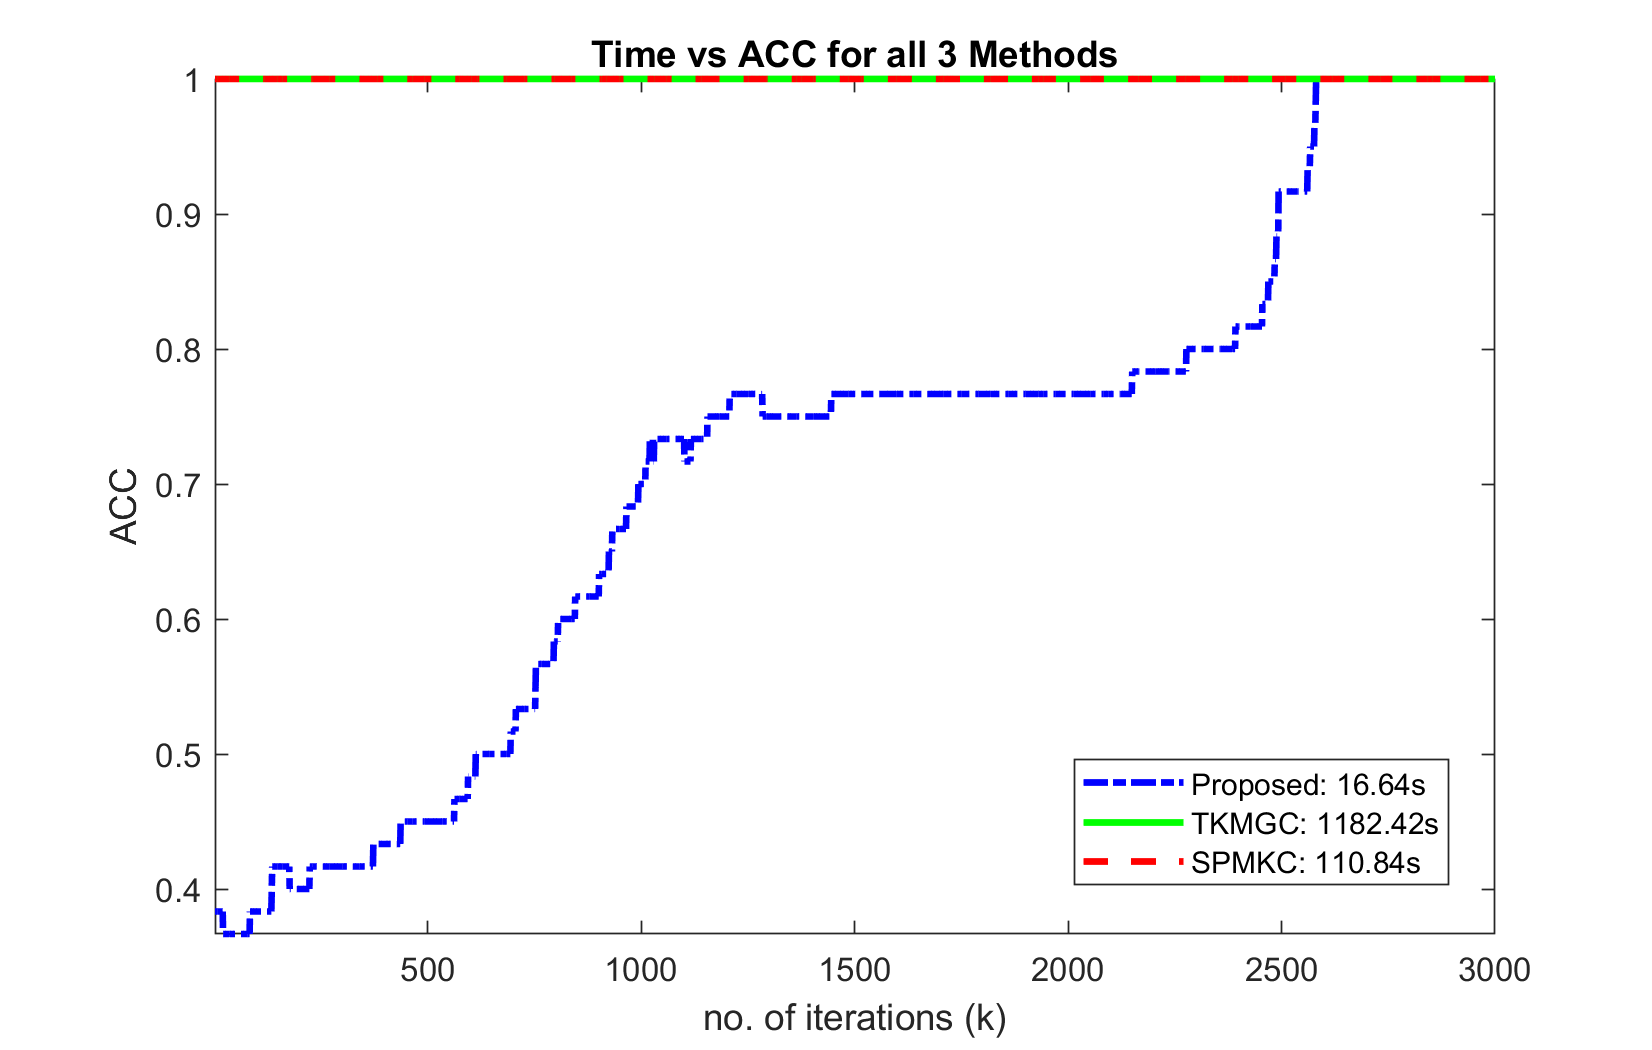
\includegraphics[scale=0.2]{acc_synthetic_plots.png}
    \caption{Time vs ACC Plots for 3 Methods with Synthetic Data}
    \label{Fig:1s}
\end{figure}
\begin{figure}[htp]
    \centering
    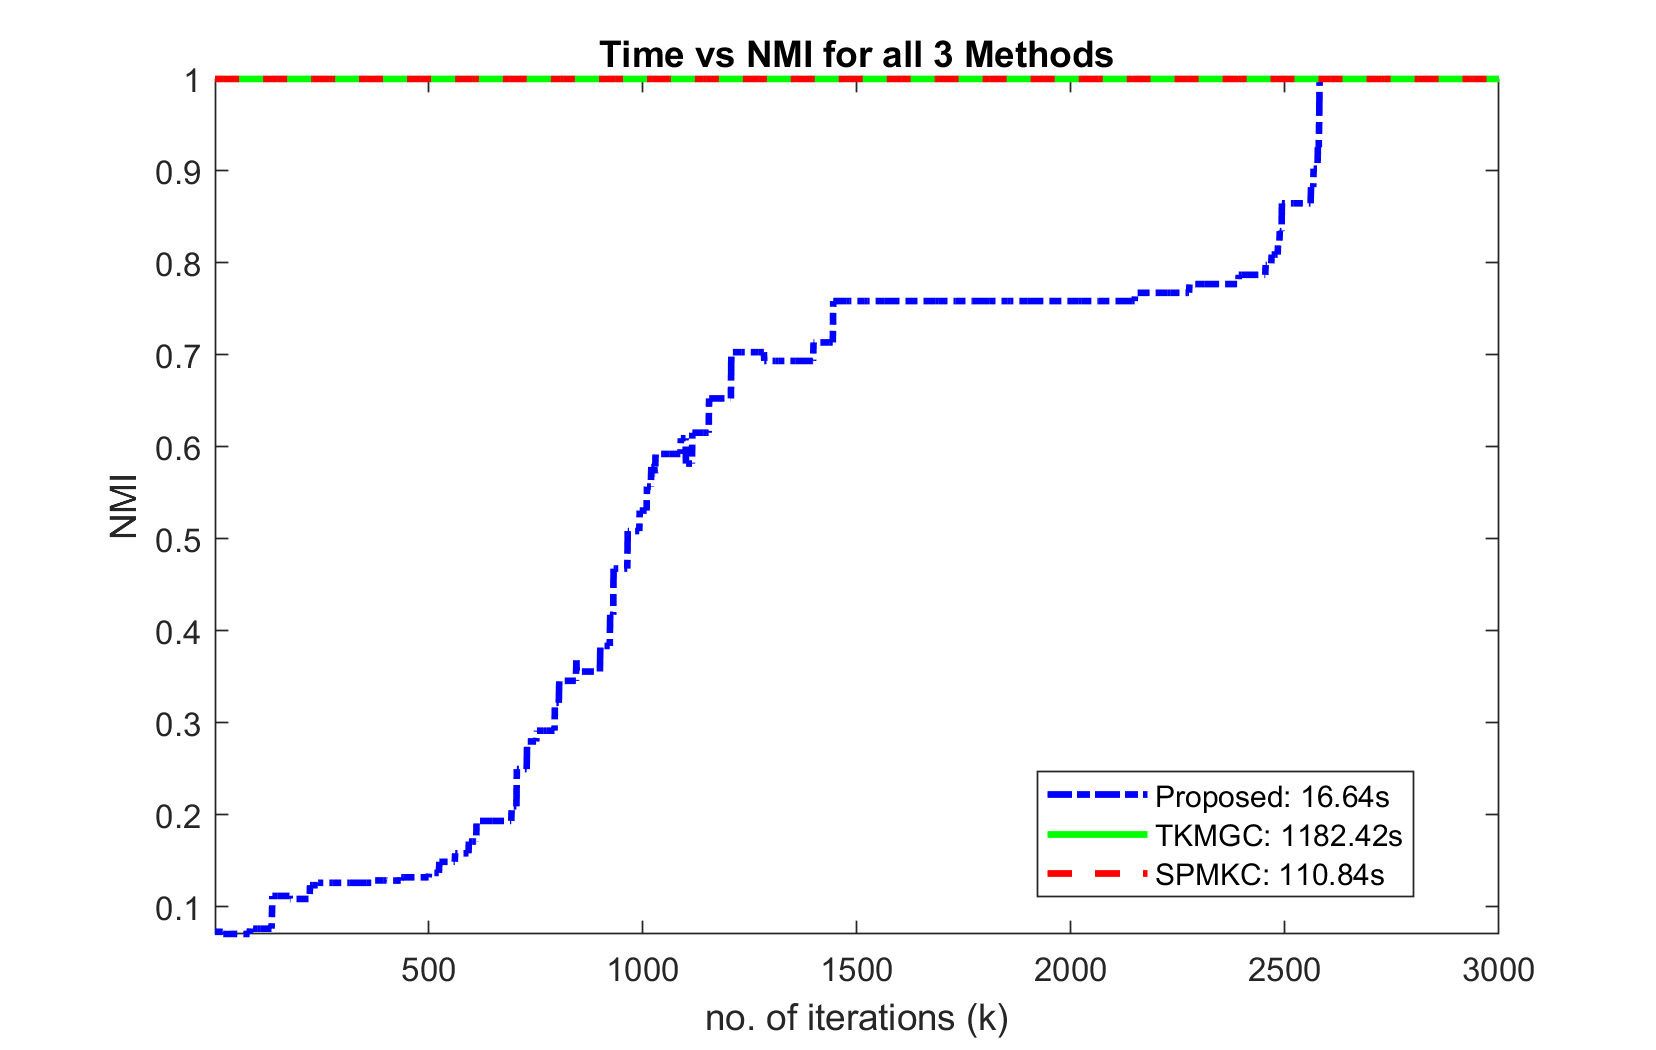
\includegraphics[scale=0.2]{nmi_synthetic_plots.png}
    \caption{Time vs NMI Plots for 3 Methods with Synthetic Data}
    \label{Fig:2s}
\end{figure}
\begin{figure}[htp]
    \centering
    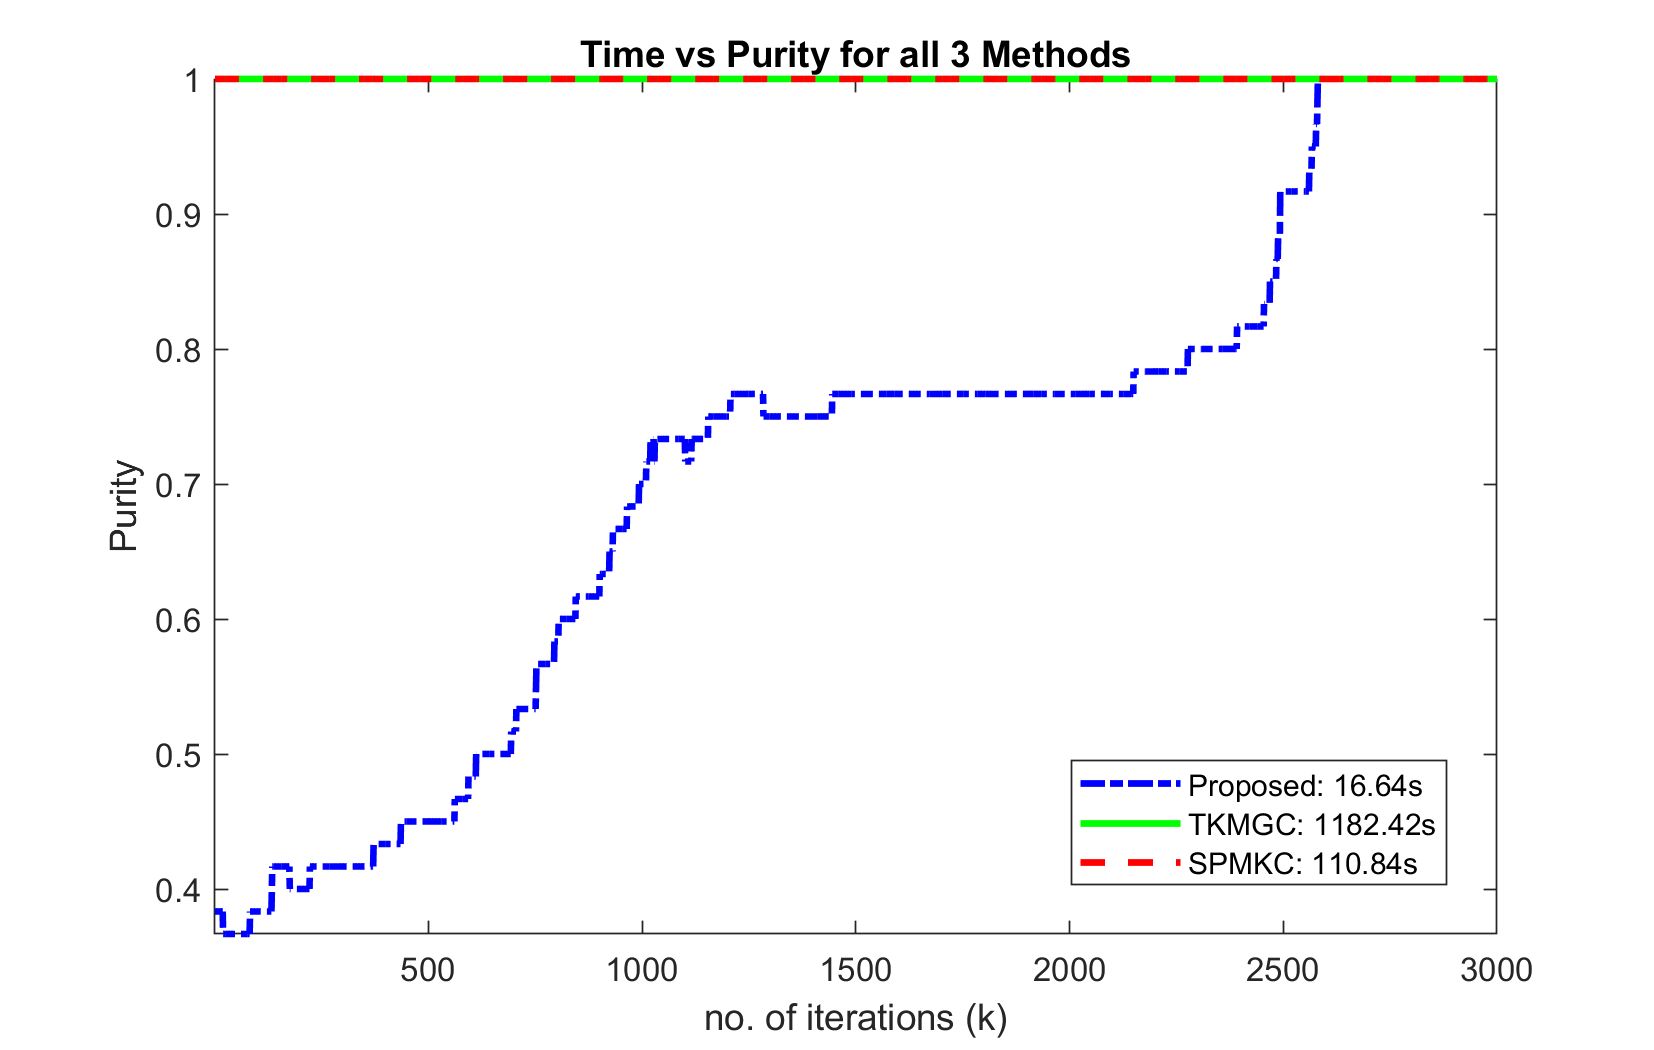
\includegraphics[scale=0.2]{purity_synthetic_plots.png}
    \caption{Time vs ACC Plots for 3 Methods with Synthetic Data}
    \label{Fig:3s}
\end{figure}
As it can be observed in Fig. 2 and 3, NMI and purity for the proposed scheme with synthetic data follow the same trend as the accuracy plot demonstrated by Fig. 1 which further bolsters the efficiency and reduced time complexity of OKC method in Alg. 1.
\begin{figure}[htp]\label{Fig_1}
    \centering
    \includegraphics[scale=0.19]{runtime_barplot.png}
    \caption{Runtime comparison across different clustering methods.}
    \label{Fig:1}
\end{figure}

Figure 5 below helps to draw a clear picture of how $\alpha_b^t$ change with time. As it can be observed in the figure, $\alpha_b^t$ for $b=1,2,3,4$ fluctuate around 0.25 from 0 to 100 iterations while the first entry of $\alpha_1^t$  drops down approximately to 0 from 100 to 200 iterations. However, during the same interval of the runtime, $\alpha_2^t$  rises to approximately 0.5 before decreasing to about 0.25. Throughout the duration of the runtime, $\alpha_3^t,\alpha_4^t$  remain fluctuating around 0.25 and $\alpha_5^t,\alpha_6^t$ remain at 0. 
%%
\begin{figure}[htp]
    \centering
    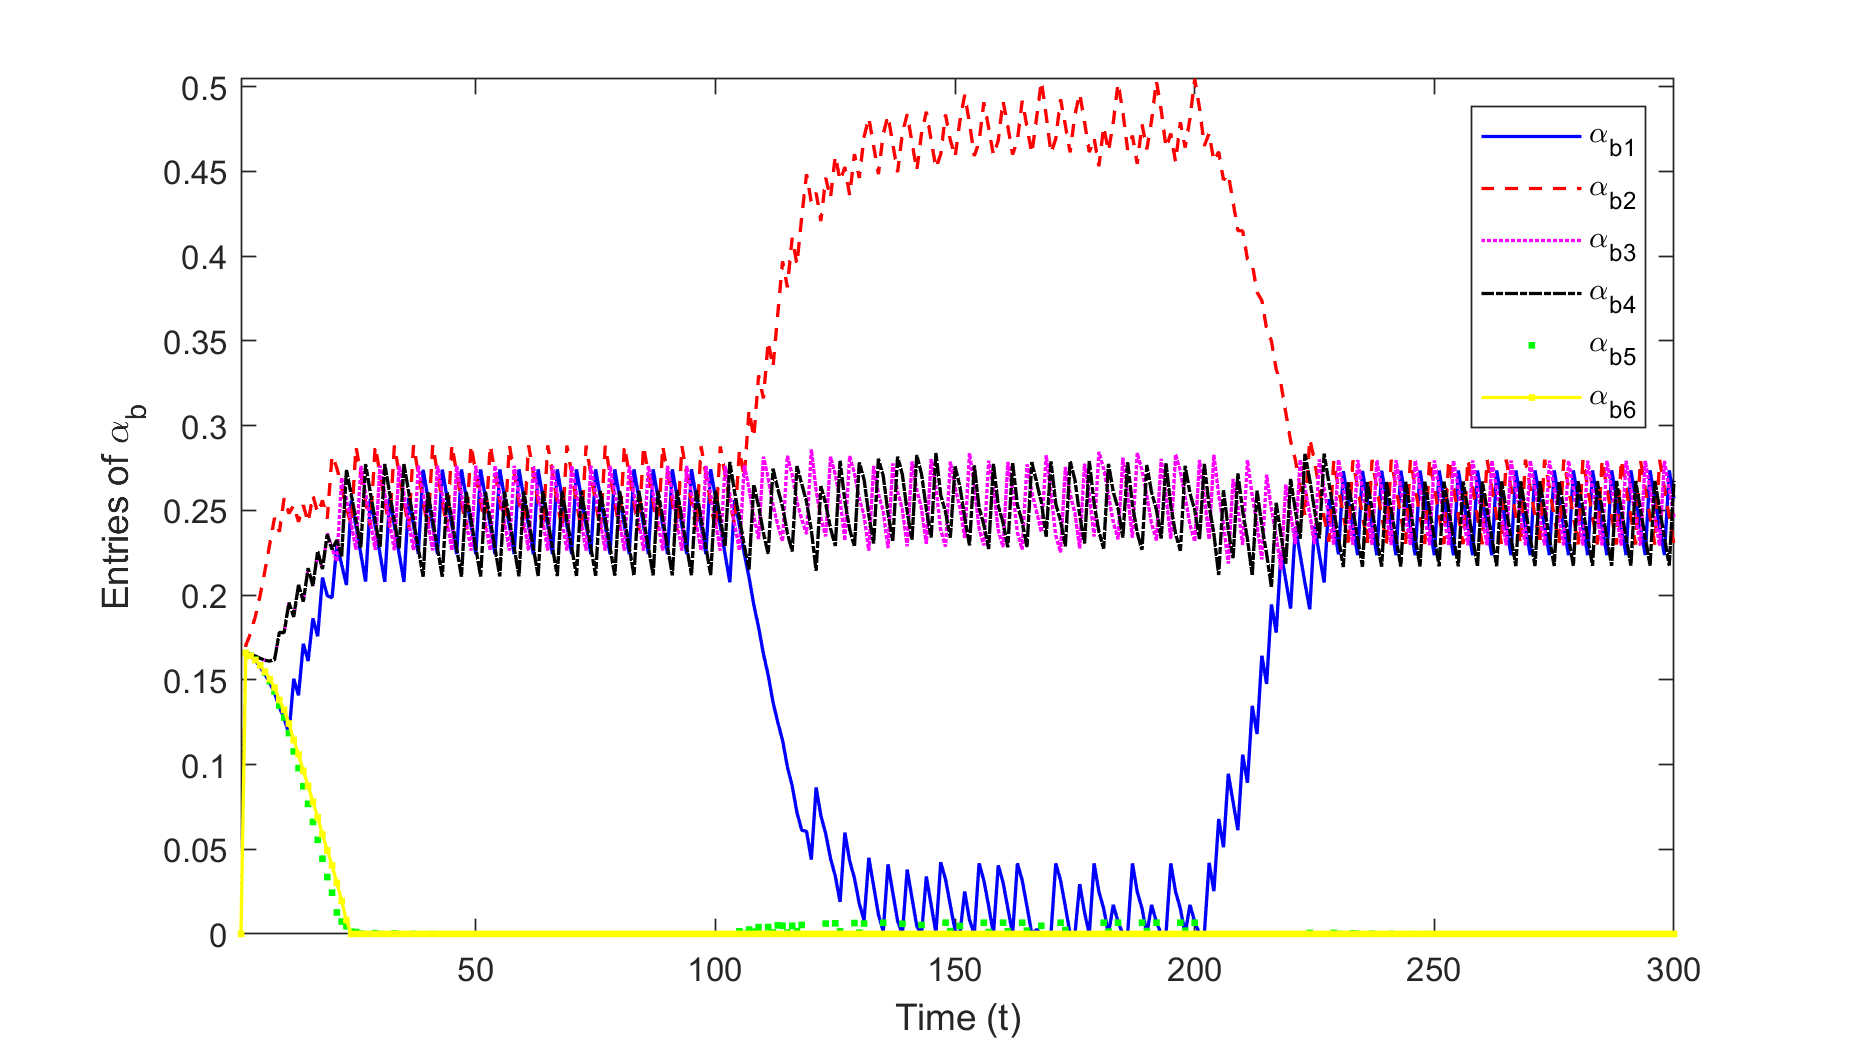
\includegraphics[scale=0.2]{tracking_entries_of_alpha_b.png}
    \caption{Tracking of kernel coefficients $\alpha_b$ vs time.}
    \label{Fig:2}
\end{figure}
%%
\subsection{Unimib Data}
The second dataset corresponds to the University of Milano Bicocca Smartphone-based Human Activity Recognition (Unimib) which consists of accelerometer readings of users that participated in numerous activities such as walking, running, and climbing stairs. The signals are pre-processed such that the data vectors are grouped into individual epochs with each of them conformed of 51 samples in length and centered around the peak of the epochs. Since the accelerometer readings are considered along all the 3-D axes, the concatenated signal is 153 samples long. The goal in this scenario is to categorize the signals based on the activity class they belong to. As stated earlier, epochs from $Q=3$ different activities are considered; walking, running, and climbing stairs.

\textcolor{black}{The first 20 vector entries of each data vector $\bbx_t$ correspond to walking, the next 20 entries correspond to running, and the last 20 entries correspond to climbing stairs. In the time-varying case, the data remains unchanged during $[1,100]$. During interval $[101,200]$ the last 20 entries gradually switch from the third type of activity to the second type of activity which corresponds to running, thereby, leading to just 2 classes; walking and running. Then, during interval $[201,300]$, the last 20 entries switch back corresponding to the third type of activity, increasing the number of classes back to 3.} The highest accuracy, purity and NMI metrics achieved by the novel OKC framework are provided for the three different intervals  $[1,100]$, $[101,200]$ and $[201,300]$ in Table I. Similarly, the same results are provided for TKMGC, SPMKC and K-means in Tables II, III and IV respectively. 

\begin{center}
\begin{table}[h!]
\begin{tabular}{|c|c|c|c|c|c|c|c|c|}
    \hline
    \multicolumn{3}{|c|}{0-100} & \multicolumn{3}{|c|}{1001-200} & \multicolumn{3}{|c|}{2001-300}\\
    \hline
    ACC & NMI & PUR & ACC & NMI & PUR & ACC & NMI & PUR\\
    \hline
    0.75 & 0.43 & 0.75 & 0.85 & 0.35 & 0.85 & 0.67 & 0.30 & 0.67\\
    0.58 & 0.28 & 0.60 & 0.61 & 0.06 & 0.67 & 0.65 & 0.29 & 0.65\\
    0.53 & 0.18 & 0.53 & 0.67 & 0.04 & 0.67 & 0.45 & 0.04 & 0.45\\
    0.98 & 0.93 & 0.98 & 0.60 & 0.03 & 0.67 & 0.79 & 0.56 & 0.79\\
    0.70 & 0.28 & 0.70 & 0.65 & 0.04 & 0.67 & 0.55 & 0.32 & 0.55\\
    0.96 & 0.86 & 0.96 & 0.85 & 0.42 & 0.85 & 0.75 & 0.54 & 0.75\\
    0.55 & 0.15 & 0.55 & 0.63 & 0.01 & 0.67 & 0.45 & 0.04 & 0.45\\
    0.88 & 0.66 & 0.88 & 0.82 & 0.38 & 0.82 & 0.72 & 0.47 & 0.72\\
    0.65 & 0.34 & 0.65 & 0.69 & 0.17 & 0.69 & 0.67 & 0.46 & 0.67\\
    0.54 & 0.09 & 0.54 & 0.65 & 0.05 & 0.67 & 0.54 & 0.09 & 0.54\\
    0.80 & 0.46 & 0.80 & 0.85 & 0.37 & 0.85 & 0.75 & 0.51 & 0.75\\
    0.66 & 0.26 & 0.66 & 0.77 & 0.19 & 0.77 & 0.64 & 0.30 & 0.64\\
    0.71 & 0.49 & 0.71 & 0.78 & 0.18 & 0.78 & 0.74 & 0.37 & 0.74\\
    0.63 & 0.20 & 0.63 & 0.82 & 0.34 & 0.82 & 0.78 & 0.51 & 0.78\\
    0.77 & 0.57 & 0.77 & 0.88 & 0.53 & 0.88 & 0.80 & 0.63 & 0.80\\
    0.69 & 0.50 & 0.69 & 0.90 & 0.57 & 0.90 & 0.67 & 0.42 & 0.67\\
    0.74 & 0.39 & 0.74 & 0.81 & 0.38 & 0.81 & 0.72 & 0.27 & 0.72\\
    0.88 & 0.66 & 0.88 & 0.83 & 0.37 & 0.83 & 0.62 & 0.39 & 0.62\\
    0.83 & 0.57 & 0.83 & 0.80 & 0.32 & 0.80 & 0.70 & 0.36 & 0.70\\
    0.71 & 0.39 & 0.71 & 0.77 & 0.37 & 0.77 & 0.72 & 0.43 & 0.72\\
    0.83 & 0.55 & 0.83 & 0.74 & 0.17 & 0.74 & 0.88 & 0.73 & 0.88\\
    0.82 & 0.66 & 0.82 & 0.88 & 0.53 & 0.88 & 0.74 & 0.56 & 0.74\\
    0.90 & 0.84 & 0.90 & 0.97 & 0.77 & 0.97 & 0.75 & 0.46 & 0.75\\
    0.83 & 0.59 & 0.83 & 0.92 & 0.65 & 0.92 & 0.65 & 0.38 & 0.65\\
    0.70 & 0.38 & 0.70 & 0.86 & 0.50 & 0.86 & 0.77 & 0.45 & 0.77\\
    0.83 & 0.61 & 0.83 & 0.72 & 0.11 & 0.72 & 0.60 & 0.19 & 0.60\\
    0.74 & 0.55 & 0.74 & 0.80 & 0.41 & 0.80 & 0.72 & 0.42 & 0.72\\
    0.79 & 0.53 & 0.79 & 0.85 & 0.36 & 0.85 & 0.69 & 0.50 & 0.69\\
    \hline
\end{tabular}
\caption{\label{tab:Table I}Accuracy, NMI, and Purity of OKC  applied in Unimib dataset.}
\end{table}
\end{center}

% \begin{center}
%     \begin{table}[h!]
%         \centering
%         \begin{tabular}{|p{1cm}|p{2cm}|p{2cm}|p{2cm}|}
%         \hline
%         \multicolumn{4}{|c|}{Iterations from 1 to 100} \\
%         \hline
%         Index & ACC & NMI & Purity \\
%         \hline
%         % \multirow{30}{2em}{OKC} 
%         & 0.75 & 0.43 & 0.75 \\
%         & 0.58 & 0.28 & 0.60 \\
%         & 0.53 & 0.18 & 0.53 \\
%         & 0.98 & 0.93 & 0.98 \\
%         & 0.70 & 0.28 & 0.70 \\
%         & 0.96 & 0.86 & 0.96 \\
%         & 0.55 & 0.15 & 0.55 \\
%         & 0.88 & 0.66 & 0.88 \\
%         & 0.65 & 0.34 & 0.65 \\
%         & 0.54 & 0.09 & 0.54 \\
%         & 0.80 & 0.46 & 0.80 \\
%         & 0.66 & 0.26 & 0.66 \\
%         & 0.71 & 0.49 & 0.71 \\
%         & 0.63 & 0.20 & 0.63 \\
%         & 0.77 & 0.57 & 0.77 \\
%         & 0.69 & 0.50 & 0.69 \\
%         & 0.74 & 0.39 & 0.74 \\
%         & 0.88 & 0.66 & 0.88 \\
%         & 0.83 & 0.57 & 0.83 \\
%         & 0.71 & 0.39 & 0.71 \\
%         & 0.83 & 0.55 & 0.83 \\
%         & 0.82 & 0.66 & 0.82 \\
%         & 0.90 & 0.84 & 0.90 \\
%         & 0.83 & 0.59 & 0.83 \\
%         & 0.70 & 0.38 & 0.70 \\
%         & 0.83 & 0.61 & 0.83 \\
%         & 0.74 & 0.55 & 0.74 \\
%         & 0.79 & 0.53 & 0.79 \\
%         \hline
%         \multirow{30}{2em}{TKMGC} 
%         & 0.74 & 0.50 & 0.83 \\
%         & 0.49 & 0.23 & 0.60 \\
%         & 0.39 & 0.13 & 0.52 \\
%         & 0.72 & 0.66 & 0.92 \\
%         & 0.50 & 0.36 & 0.67 \\
%         & 0.62 & 0.45 & 0.77 \\
%         & 0.50 & 0.23 & 0.57 \\
%         & 0.75 & 0.53 & 0.85 \\
%         & 0.71 & 0.50 & 0.81 \\
%         & 0.50 & 0.24 & 0.58 \\
%         & 0.62 & 0.43 & 0.75 \\
%         & 0.44 & 0.14 & 0.51 \\
%         & 0.58 & 0.49 & 0.69 \\
%         & 0.49 & 0.43 & 0.63 \\
%         & 0.58 & 0.47 & 0.70 \\
%         & 0.62 & 0.44 & 0.77 \\
%         & 0.56 & 0.32 & 0.67 \\
%         & 0.74 & 0.60 & 0.90 \\
%         & 0.67 & 0.46 & 0.78 \\
%         & 0.55 & 0.24 & 0.67 \\
%         & 0.79 & 0.62 & 0.90 \\
%         & 0.67 & 0.45 & 0.77 \\
%         & 0.87 & 0.74 & 0.97 \\
%         & 0.79 & 0.64 & 0.89 \\
%         & 0.61 & 0.40 & 0.72 \\
%         & 0.65 & 0.52 & 0.79 \\
%         & 0.64 & 0.46 & 0.76 \\
%         & 0.65 & 0.46 & 0.78 \\
%         \multirow{30}{2em}{SPMKC} 
%         & 0.71 & 0.41 & 0.71 \\
%         & 0.45 & 0.30 & 0.79 \\
%         & 0.46 & 0.15 & 0.61 \\
%         & 0.75 & 0.51 & 0.75 \\
%         & 0.50 & 0.33 & 0.63 \\
%         & 0.54 & 0.17 & 0.70 \\
%         & 0.60 & 0.24 & 0.68 \\
%         & 0.53 & 0.32 & 0.81 \\
%         & 0.58 & 0.35 & 0.78 \\
%         & 0.58 & 0.23 & 0.71 \\
%         & 0.47 & 0.34 & 0.80 \\
%         & 0.49 & 0.23 & 0.53 \\
%         & 0.50 & 0.25 & 0.61 \\
%         & 0.46 & 0.27 & 0.79 \\
%         & 0.53 & 0.23 & 0.69 \\
%         & 0.54 & 0.39 & 0.83 \\
%         & 0.41 & 0.17 & 0.85 \\
%         & 0.48 & 0.14 & 0.48 \\
%         & 0.59 & 0.26 & 0.70 \\
%         & 0.69 & 0.40 & 0.71 \\
%         & 0.60 & 0.58 & 0.93 \\
%         & 0.81 & 0.56 & 0.81 \\
%         & 0.40 & 0.15 & 0.87 \\
%         & 0.44 & 0.08 & 0.62 \\
%         & 0.48 & 0.27 & 0.63 \\
%         & 0.76 & 0.51 & 0.81 \\
%         & 0.48 & 0.30 & 0.81 \\
%         & 0.74 & 0.49 & 0.80 \\
%         \hline
%         \multirow{30}{2em}{KMEANS} 
%         & 0.80 & 0.55 & 0.80 \\
%         & 0.73 & 0.46 & 0.73 \\
%         & 0.53 & 0.20 & 0.53 \\
%         & 0.63 & 0.34 & 0.63 \\
%         & 0.85 & 0.59 & 0.85 \\
%         & 0.66 & 0.46 & 0.66 \\
%         & 0.57 & 0.26 & 0.57 \\
%         & 0.79 & 0.55 & 0.79 \\
%         & 0.83 & 0.68 & 0.83 \\
%         & 0.60 & 0.26 & 0.60 \\
%         & 0.73 & 0.46 & 0.73 \\
%         & 0.66 & 0.30 & 0.65 \\
%         & 0.67 & 0.43 & 0.67 \\
%         & 0.68 & 0.48 & 0.68 \\
%         & 0.67 & 0.36 & 0.67 \\
%         & 0.71 & 0.49 & 0.70 \\
%         & 0.69 & 0.38 & 0.69 \\
%         & 0.60 & 0.31 & 0.60 \\
%         & 0.69 & 0.45 & 0.69 \\
%         & 0.63 & 0.34 & 0.63 \\
%         & 0.67 & 0.31 & 0.67 \\
%         & 0.82 & 0.60 & 0.82 \\
%         & 0.78 & 0.58 & 0.78 \\
%         & 0.56 & 0.29 & 0.56 \\
%         & 0.54 & 0.21 & 0.54 \\
%         & 0.86 & 0.71 & 0.86 \\
%         & 0.68 & 0.48 & 0.68 \\
%         & 0.77 & 0.44 & 0.77 \\
%         \end{tabular}
%         \caption{Caption}
%         \label{tab:my_label}
%     \end{table}
% \end{center}


\begin{center}
\begin{table*}[h!]
\begin{tabular}{|c|c|c|c|c|c|c|c|c|c|c|c|c|}
   \hline
   \multicolumn{1}{|c|}{}&\multicolumn{4}{|c|}{ACC} & \multicolumn{4}{|c|}{NMI} & \multicolumn{4}{|c|}{Purity}\\
   \cline{2-13}
   Index & OKC & TKMGC & SPMKC & K-Means & OKC & TKMGC & SPMKC & K-Means & OKC & TKMGC & SPMKC & K-Means \\
   \hline
   1 & 0.75	&	0.74	&	0.71	&	0.8	&	0.43	&	0.5	&	0.41	&	0.55	&	 0.75	&	0.83	&	0.71	&	0.8\\
	2 & 0.58	&	0.49	&	0.45	&	0.73	&	0.28	&	0.23	&	0.3	&	0.46	&	 0.60 	&	0.6	&	0.79	&	0.73\\
	3 & 0.53	&	0.39	&	0.46	&	0.53	&	0.18	&	0.13	&	0.15	&	0.2	&	 0.53 	&	0.52	&	0.61	&	0.53\\
	4 & 0.98	&	0.72	&	0.75	&	0.63	&	0.93	&	0.66	&	0.51	&	0.34	&	 0.98 	&	0.92	&	0.75	&	0.63\\
	5 & 0.7	&	0.5	&	0.5	&	0.85	&	0.28	&	0.36	&	0.33	&	0.59	&	 0.70 	&	0.67	&	0.63	&	0.85\\
	6 & 0.96	&	0.62	&	0.54	&	0.66	&	0.86	&	0.45	&	0.17	&	0.46	&	 0.96 	&	0.77	&	0.7	&	0.66\\
	7 & 0.55	&	0.5	&	0.6	&	0.57	&	0.15	&	0.23	&	0.24	&	0.26	&	 0.55 	&	0.57	&	0.68	&	0.57\\
	8 & 0.88	&	0.75	&	0.53	&	0.79	&	0.66	&	0.53	&	0.32	&	0.55	&	 0.88	&	0.85	&	0.81	&	0.79\\
	9 & 0.65	&	0.71	&	0.58	&	0.83	&	0.34	&	0.5	&	0.35	&	0.68	&	 0.65	&	0.81	&	0.78	&	0.83\\
	10 & 0.54	&	0.5	&	0.58	&	0.6	&	0.09	&	0.24	&	0.23	&	0.26	&	 0.54	&	0.58	&	0.71	&	0.6\\
	11 & 0.8	&	0.62	&	0.47	&	0.73	&	0.46	&	0.43	&	0.34	&	0.46	&	 0.80	&	0.75	&	0.8	&	0.73\\
	12 & 0.66	&	0.44	&	0.49	&	0.66	&	0.26	&	0.14	&	0.23	&	0.3	&	 0.66	&	0.51	&	0.53	&	0.65\\
	13 & 0.71	&	0.58	&	0.5	&	0.67	&	0.49	&	0.49	&	0.25	&	0.43	&	 0.71	&	0.69	&	0.61	&	0.67\\
	14 & 0.63	&	0.49	&	0.46	&	0.68	&	0.2	&	0.43	&	0.27	&	0.48	&	 0.63	&	0.63	&	0.79	&	0.68\\
	15 & 0.77	&	0.58	&	0.53	&	0.67	&	0.57	&	0.47	&	0.23	&	0.36	&	 0.77	&	0.7	&	0.69	&	0.67\\
	16 & 0.69	&	0.62	&	0.54	&	0.71	&	0.5	&	0.44	&	0.39	&	0.49	&	 0.69	&	0.77	&	0.83	&	0.7\\
	17 & 0.74	&	0.56	&	0.41	&	0.69	&	0.39	&	0.32	&	0.17	&	0.38	&	 0.74	&	0.67	&	0.85	&	0.69\\
	18 & 0.88	&	0.74	&	0.48	&	0.6	&	0.66	&	0.6	&	0.14	&	0.31	&	 0.88	&	0.9	&	0.48	&	0.6\\
	19 & 0.83	&	0.67	&	0.59	&	0.69	&	0.57	&	0.46	&	0.26	&	0.45	&	 0.83	&	0.78	&	0.7	&	0.69\\
	20 & 0.71	&	0.55	&	0.69	&	0.63	&	0.39	&	0.24	&	0.4	&	0.34	&	 0.71	&	0.67	&	0.71	&	0.63\\
	21 & 0.83	&	0.79	&	0.6	&	0.67	&	0.55	&	0.62	&	0.58	&	0.31	&	 0.83	&	0.9	&	0.93	&	0.67\\
	22 & 0.82	&	0.67	&	0.81	&	0.82	&	0.66	&	0.45	&	0.56	&	0.6	&	 0.82	&	0.77	&	0.81	&	0.82\\
	23 & 0.9	&	0.87	&	0.4	&	0.78	&	0.84	&	0.74	&	0.15	&	0.58	&	 0.90	&	0.97	&	0.87	&	0.78\\
	24 & 0.83	&	0.79	&	0.44	&	0.56	&	0.59	&	0.64	&	0.08	&	0.29	&	 0.83	&	0.89	&	0.62	&	0.56\\
	25 & 0.7	&	0.61	&	0.48	&	0.54	&	0.38	&	0.4	&	0.27	&	0.21	&	 0.70	&	0.72	&	0.63	&	0.54\\
	26 & 0.83	&	0.65	&	0.76	&	0.86	&	0.61	&	0.52	&	0.51	&	0.71	&	 0.83	&	0.79	&	0.81	&	0.86\\
	27 & 0.74	&	0.64	&	0.48	&	0.68	&	0.55	&	0.46	&	0.3	&	0.48	&	 0.74	&	0.76	&	0.81	&	0.68\\
	28 & 0.79	&	0.65	&	0.74	&	0.77	&	0.53	&	0.46	&	0.49	&	0.44	&	 0.79	&	0.78	&	0.8	&	0.77\\
   \hline
\end{tabular}
\caption{\label{tab:Table I}Accuracy, NMI, and Purity of different methods  applied to Unimib dataset for iterations 1 to 100.}
\end{table*}
\end{center}
\subsection{Salinas Data}
The third set of data used is a hyperspectral image dataset captured by an Aviris sensing system over the Salinas valley, California. These are primarily farmland images that indicate the presence of different crops/materials in different parts of the images. Each pixel denotes one out of the 16 different types of crops/materials in the images. In this scenario, the new algorithm is expected to analyze each pixel independently and cluster them based on the 224 dimension vector into different classes based on the crop/material they belong to.  A total of $Q=4$ different randomly selected materials were considered and $25$ random pixels were chosen for each of the $4$ classes. 

\textcolor{black}{{In the Salinas dataset the $100\times 1$ data vectors $\bbx_t$ contain information about four different materials. During time frame $[1,100]$ $25$ entries are allocated to each of the four different classes. During time frame  $[101,200]$ the $25$ entries corresponding to class 3 are switched  with data entries corresponding to class 4, thereby, switching the number of classes/clusters present in the data from $Q=4$ to $Q=3$. During time frame $[201,300]$, the $25$ data entries that were replaced with data from class $4$ are switched back to data entries corresponding to class $3$, increasing the number of underlying clusters back to $Q=4$.}}
%\begin{tabular}{|c|c|c|c|c|c|c|c|c|}
%    \hline
%    \multicolumn{3}{|c|}{0-1000} & \multicolumn{3}{|c|}{1001-2000} & \multicolumn{3}{|c|}{2001-3000}\\
%    \hline
%    ACC & NMI & PUR & ACC & NMI & PUR & ACC & NMI & PUR\\
%    \hline
%    0.89 & 0.80 & 0.89 & 0.73 & 0.59 & 0.75 & 0.87 & 0.73 & 0.87\\
%    0.98 & 0.94 & 0.98 & 0.74 & 0.63 & 0.74 & 0.98 & 0.94 & 0.98\\
%    0.81 & 0.71 & 0.81 & 0.73 & 0.59 & 0.74 & 0.88 & 0.79 & 0.88\\
%    0.61 & 0.43 & 0.64 & 0.68 & 0.35 & 0.68 & 0.61 & 0.43 & 0.64\\
%    0.98 & 0.94 & 0.98 & 1.00 & 1.00 & 1.00 & 0.64 & 0.72 & 0.74\\
%    0.98 & 0.95 & 0.98 & 0.97 & 0.91 & 0.97 & 0.97 & 0.93 & 0.97\\
%    0.94 & 0.99 & 0.94 & 0.75 & 0.67 & 0.75 & 0.82 & 0.75 & 0.82\\
%    0.92 & 0.85 & 0.92 & 0.54 & 0.54 & 0.75 & 0.90 & 0.81 & 0.9\\
%    1.00 & 1.00 & 1.00 & 0.75 & 0.60 & 0.75 & 1.00 & 1.00 & 1.00\\
%    0.85 & 0.81 & 0.85 & 0.59 & 0.53 & 0.75 & 0.99 & 0.97 & 0.99\\
%    1.00 & 1.00 & 1.00 & 1.00 & 1.00 & 1.00 & 0.99 & 0.95 & 0.99\\
%    1.00 & 1.00 & 1.00 & 1.00 & 1.00 & 1.00 & 1.00 & 1.00 & 1.00\\
%    0.84 & 0.69 & 0.84 & 0.76 & 0.41 & 0.76 & 0.69 & 0.51 & 0.69\\
%    0.96 & 0.88 & 0.96 & 0.71 & 0.56 & 0.75 & 0.95 & 0.87 & 0.95\\
%    0.99 & 0.97 & 0.99 & 0.85 & 0.66 & 0.85 & 0.92 & 0.85 & 0.92\\
%    0.98 & 0.95 & 0.98 & 0.50 & 0.67 & 0.75 & 0.98 & 0.95 & 0.98\\
%    0.95 & 0.89 & 0.95 & 0.80 & 0.68 & 0.80 & 0.72 & 0.71 & 0.75\\
%    0.80 & 0.65 & 0.80 & 0.69 & 0.45 & 0.71 & 0.74 & 0.62 & 0.74\\
%    0.98 & 0.94 & 0.98 & 0.98 & 0.92 & 0.98 & 0.99 & 0.97 & 0.99\\
%    0.91 & 0.79 & 0.91 & 0.55 & 0.46 & 0.70 & 0.90 & 0.81 & 0.9\\
%    0.99 & 0.97 & 0.99 & 0.74 & 0.63 & 0.75 & 0.99 & 0.97 & 0.99\\
%    1.00 & 1.00 & 1.00 & 0.75 & 0.67 & 0.75 & 1.00 & 1.00 & 1.00\\
%    0.95 & 0.89 & 0.95 & 0.67 & 0.54 & 0.75 & 0.95 & 0.89 & 0.95\\
%    0.64 & 0.46 & 0.64 & 0.54 & 0.25 & 0.60 & 0.64 & 0.46 & 0.64\\
%    0.98 & 0.94 & 0.98 & 0.99 & 0.95 & 0.99 & 0.98 & 0.94 & 0.98\\
%    0.72 & 0.70 & 0.73 & 0.61 & 0.48 & 0.72 & 0.57 & 0.41 & 0.57\\
%    0.95 & 0.87 & 0.95 & 0.73 & 0.46 & 0.73 & 0.97 & 0.92 & 0.97\\
%    0.99 & 0.97 & 0.99 & 0.87 & 0.71 & 0.87 & 0.99 & 0.97 & 0.99\\
%    0.70 & 0.60 & 0.70 & 0.68 & 0.56 & 0.74 & 0.94 & 0.89 & 0.94\\
%    0.68 & 0.53 & 0.68 & 0.68 & 0.36 & 0.68 & 0.75 & 0.58 & 0.75\\
%    0.68 & 0.61 & 0.72 & 0.64 & 0.43 & 0.73 & 0.65 & 0.59 & 0.69\\
%    0.98 & 0.95 & 0.98 & 0.75 & 0.67 & 0.75 & 0.95 & 0.88 & 0.95\\
%    0.76 & 0.75 & 0.76 & 0.73 & 0.60 & 0.75 & 1.00 & 1.00 & 1.00\\
%    0.97 & 0.92 & 0.97 & 0.99 & 0.96 & 0.99 & 0.97 & 0.92 & 0.97\\
%    0.87 & 0.74 & 0.87 & 0.63 & 0.48 & 0.74 & 0.85 & 0.74 & 0.85\\
%    0.96 & 0.92 & 0.96 & 0.75 & 0.63 & 0.75 & 0.97 & 0.93 & 0.97\\
%    0.98 & 0.94 & 0.98 & 0.52 & 0.29 & 0.52 & 0.73 & 0.68 & 0.73\\
%    0.90 & 0.76 & 0.90 & 0.71 & 0.51 & 0.71 & 0.90 & 0.77 & 0.90\\
%    0.67 & 0.56 & 0.67 & 0.62 & 0.26 & 0.62 & 0.97 & 0.91 & 0.97\\
%    0.75 & 0.64 & 0.75 & 0.64 & 0.42 & 0.69 & 0.91 & 0.79 & 0.91\\
%    0.91 & 0.82 & 0.91 & 0.95 & 0.87 & 0.95 & 0.82 & 0.67 & 0.82\\
%    0.85 & 0.76 & 0.85 & 1.00 & 1.00 & 1.00 & 0.75 & 0.75 & 0.75\\
%    1.00 & 1.00 & 1.00 & 0.73 & 0.60 & 0.73 & 0.97 & 0.92 & 0.97\\
%    0.81 & 0.67 & 0.81 & 0.54 & 0.54 & 0.75 & 0.78 & 0.61 & 0.78\\
%    0.92 & 0.81 & 0.92 & 0.80 & 0.65 & 0.80 & 0.95 & 0.87 & 0.95\\
%    0.97 & 0.92 & 0.97 & 0.73 & 0.60 & 0.73 & 0.97 & 0.92 & 0.97\\
%    0.99 & 0.97 & 0.99 & 0.75 & 0.60 & 0.75 & 0.99 & 0.97 & 0.99\\
%    0.93 & 0.85 & 0.93 & 0.84 & 0.59 & 0.84 & 0.94 & 0.85 & 0.94\\
%    0.91 & 0.84 & 0.91 & 0.65 & 0.56 & 0.75 & 0.91 & 0.84 & 0.91\\
%    0.97 & 0.91 & 0.97 & 0.79 & 0.62 & 0.79 & 0.96 & 0.89 & 0.96\\
%    0.99 & 0.97 & 0.99 & 0.76 & 0.67 & 0.76 & 0.99 & 0.97 & 0.99\\
%    0.93 & 0.84 & 0.93 & 0.75 & 0.63 & 0.75 & 0.96 & 0.90 & 0.96\\
%    0.99 & 0.97 & 0.99 & 0.74 & 0.66 & 0.75 & 0.99 & 0.97 & 0.99\\
%    0.76 & 0.73 & 0.76 & 0.51 & 0.63 & 0.75 & 0.79 & 0.73 & 0.79\\
%    0.85 & 0.74 & 0.85 & 0.55 & 0.55 & 0.75 & 0.62 & 0.46 & 0.62\\
%    0.84 & 0.78 & 0.84 & 0.75 & 0.67 & 0.75 & 0.84 & 0.78 & 0.84\\
%    0.98 & 0.95 & 0.98 & 0.75 & 0.67 & 0.75 & 0.98 & 0.95 & 0.98\\
%    0.97 & 0.93 & 0.97 & 0.93 & 0.81 & 0.93 & 0.97 & 0.93 & 0.97\\
%    1.00 & 1.00 & 1.00 & 0.75 & 0.67 & 0.75 & 1.00 & 1.00 & 1.00\\
%    0.93 & 0.84 & 0.93 & 0.77 & 0.64 & 0.77 & 0.93 & 0.84 & 0.93\\
%    0.95 & 0.90 & 0.95 & 0.75 & 0.67 & 0.75 & 0.97 & 0.93 & 0.97\\
%    0.70 & 0.62 & 0.73 & 0.62 & 0.35 & 0.69 & 0.70 & 0.62 & 0.73\\
%    0.98 & 0.95 & 0.98 & 0.80 & 0.68 & 0.80 & 0.99 & 0.97 & 0.99\\
%    1.00 & 1.00 & 1.00 & 0.50 & 0.67 & 0.75 & 1.00 & 1.00 & 1.00\\
%    0.92 & 0.85 & 0.92 & 0.75 & 0.67 & 0.75 & 0.91 & 0.84 & 0.91\\
%    0.93 & 0.85 & 0.93 & 0.71 & 0.52 & 0.71 & 0.94 & 0.87 & 0.94\\
%    0.95 & 0.89 & 0.95 & 0.95 & 0.82 & 0.95 & 0.95 & 0.87 & 0.95\\
%    0.95 & 0.89 & 0.95 & 0.74 & 0.63 & 0.74 & 0.99 & 0.97 & 0.99\\
%    0.92 & 0.82 & 0.92 & 0.95 & 0.85 & 0.95 & 0.91 & 0.80 & 0.91\\
%    0.68 & 0.58 & 0.68 & 0.65 & 0.28 & 0.65 & 0.67 & 0.55 & 0.69\\
%    0.97 & 0.92 & 0.97 & 0.75 & 0.59 & 0.75 & 0.97 & 0.92 & 0.97\\
%    0.75 & 0.75 & 0.75 & 0.75 & 0.67 & 0.75 & 0.96 & 0.92 & 0.96\\
%    0.74 & 0.68 & 0.75 & 0.75 & 0.67 & 0.75 & 0.98 & 0.95 & 0.98\\
%    0.85 & 0.70 & 0.85 & 0.55 & 0.51 & 0.75 & 0.86 & 0.71 & 0.86\\
%    0.99 & 0.97 & 0.99 & 0.75 & 0.67 & 0.75 & 1.00 & 1.00 & 1.00\\
%    0.71 & 0.64 & 0.74 & 0.60 & 0.52 & 0.75 & 0.71 & 0.64 & 0.74\\
%    0.76 & 0.68 & 0.76 & 0.60 & 0.39 & 0.60 & 0.76 & 0.68 & 0.76\\
%    0.90 & 0.89 & 0.90 & 0.75 & 0.67 & 0.75 & 0.75 & 0.71 & 0.75\\
%    0.75 & 0.72 & 0.75 & 0.51 & 0.67 & 0.75 & 0.86 & 0.77 & 0.86\\
%    0.72 & 0.60 & 0.72 & 0.77 & 0.60 & 0.77 & 0.93 & 0.83 & 0.93\\
%    0.96 & 0.90 & 0.96 & 0.52 & 0.57 & 0.75 & 0.97 & 0.93 & 0.97\\
%    0.87 & 0.75 & 0.87 & 0.68 & 0.48 & 0.69 & 0.88 & 0.78 & 0.88\\
%    0.92 & 0.82 & 0.92 & 0.87 & 0.68 & 0.87 & 0.90 & 0.77 & 0.90\\
%    0.99 & 0.97 & 0.99 & 0.74 & 0.59 & 0.74 & 1.00 & 1.00 & 1.00\\
%    0.64 & 0.72 & 0.74 & 0.54 & 0.39 & 0.60 & 0.57 & 0.60 & 0.68\\
%    0.99 & 0.97 & 0.99 & 0.75 & 0.67 & 0.75 & 0.99 & 0.97 & 0.99\\
%    1.00 & 1.00 & 1.00 & 0.75 & 0.67 & 0.75 & 1.00 & 1.00 & 1.00\\
%    0.66 & 0.52 & 0.66 & 0.55 & 0.31 & 0.67 & 0.62 & 0.50 & 0.62\\
%    0.78 & 0.73 & 0.78 & 0.73 & 0.62 & 0.74 & 0.98 & 0.94 & 0.98\\
%    1.00 & 1.00 & 1.00 & 0.75 & 0.67 & 0.75 & 1.00 & 1.00 & 1.00\\
%    0.73 & 0.67 & 0.75 & 0.84 & 0.71 & 0.84 & 0.99 & 0.97 & 0.99\\
%    0.91 & 0.82 & 0.91 & 0.66 & 0.46 & 0.74 & 0.89 & 0.77 & 0.89\\
%    0.93 & 0.84 & 0.93 & 0.66 & 0.48 & 0.73 & 0.94 & 0.85 & 0.94\\
%    0.99 & 0.97 & 0.99 & 0.81 & 0.66 & 0.81 & 0.99 & 0.97 & 0.99\\
%    0.99 & 0.97 & 0.99 & 0.79 & 0.68 & 0.79 & 0.99 & 0.97 & 0.99\\
%    0.96 & 0.90 & 0.96 & 0.74 & 0.63 & 0.75 & 0.96 & 0.90 & 0.96\\
%    0.96 & 0.90 & 0.96 & 0.69 & 0.55 & 0.75 & 0.97 & 0.93 & 0.97\\
%    0.98 & 0.95 & 0.98 & 0.75 & 0.67 & 0.75 & 0.99 & 0.97 & 0.99\\
%    0.99 & 0.97 & 0.99 & 0.53 & 0.55 & 0.75 & 0.99 & 0.97 & 0.99\\
%    \hline
%\end{tabular}
\subsection{Comparing Other Methods}
Detailed comparisons of the novel OKC approach  with the methods TKMGC, SPMKC, and K-means follow next. %TKMGC and SPMKC are multiple kernel learning methods that were developed in response to solving the issues of high-dimensional clustering by forming low-dimensional subspaces corresponding to a specific class or group. Both TKMGC and SPMKC rely on a kernel pool comprised of m base kernels \begin{math}{H^{k}_{k=1}^{m}\end{math} derived from data matrices of n samples. In these scenarios, the data matrices used are the synthetic, Unimib, and Salinas datasets each containing a different number of sample points. 
Fine tuning of TKMGC boils down to properly setting parameters \begin{math}\alpha\end{math} and \begin{math}\beta\end{math} to cluster data accordingly. These two parameters  were fine tuned to have values between \begin{math}10^{-5}\end{math} and \begin{math}10^2\end{math} which enabled TKMGC to achieve the best possible  accuracy, NMI, and purity. The best values were acquired at \begin{math}\alpha=10^{-1}\end{math} and \begin{math}\beta=10^{-3}\end{math} for Unimib, while for Salinas the parameters were set as \begin{math}\alpha=10\end{math} and \begin{math}\beta=10^{-4}\end{math}. 

Similarly, SPMKC was tuned using the parameters \begin{math}\lambda_1\end{math} and \begin{math}\lambda_3\end{math}. Although there are a total of 4 parameters used in SPMKC, according to \textcolor{black}{\cite{SPMKC}}, \begin{math}\lambda_2\end{math} is set to one and \begin{math}\lambda_4\end{math} is fixed at 1 for best results. Parameters \begin{math}\lambda_1\end{math} and \begin{math}\lambda_3\end{math} are selected from the sets $\{1,2,3,4,5,6\}$ and $\{1,10,100,200,400,1000\}$ respectively. Several combinations of \begin{math}\lambda_1\end{math} and \begin{math}\lambda_3\end{math} were implemented to achieve the best clustering performance. It was found that \begin{math}\lambda_1=4\end{math} and \begin{math}\lambda_3=400\end{math} generated the highest accuracy, NMI, and purity for Unimib, while \begin{math}\lambda_1=6\end{math} and \begin{math}\lambda_3=200\end{math} worked best for Salinas. Figures \ref{Fig:3u},\ref{Fig:4u} and \ref{Fig:5u} below depict accuracy versus time, NMI versus time, and purity versus time plots for OKC, TMKGC, SPMKC and K-means when applied on the time-varying Unimib dataset.
\begin{figure}[htp]
    \centering
    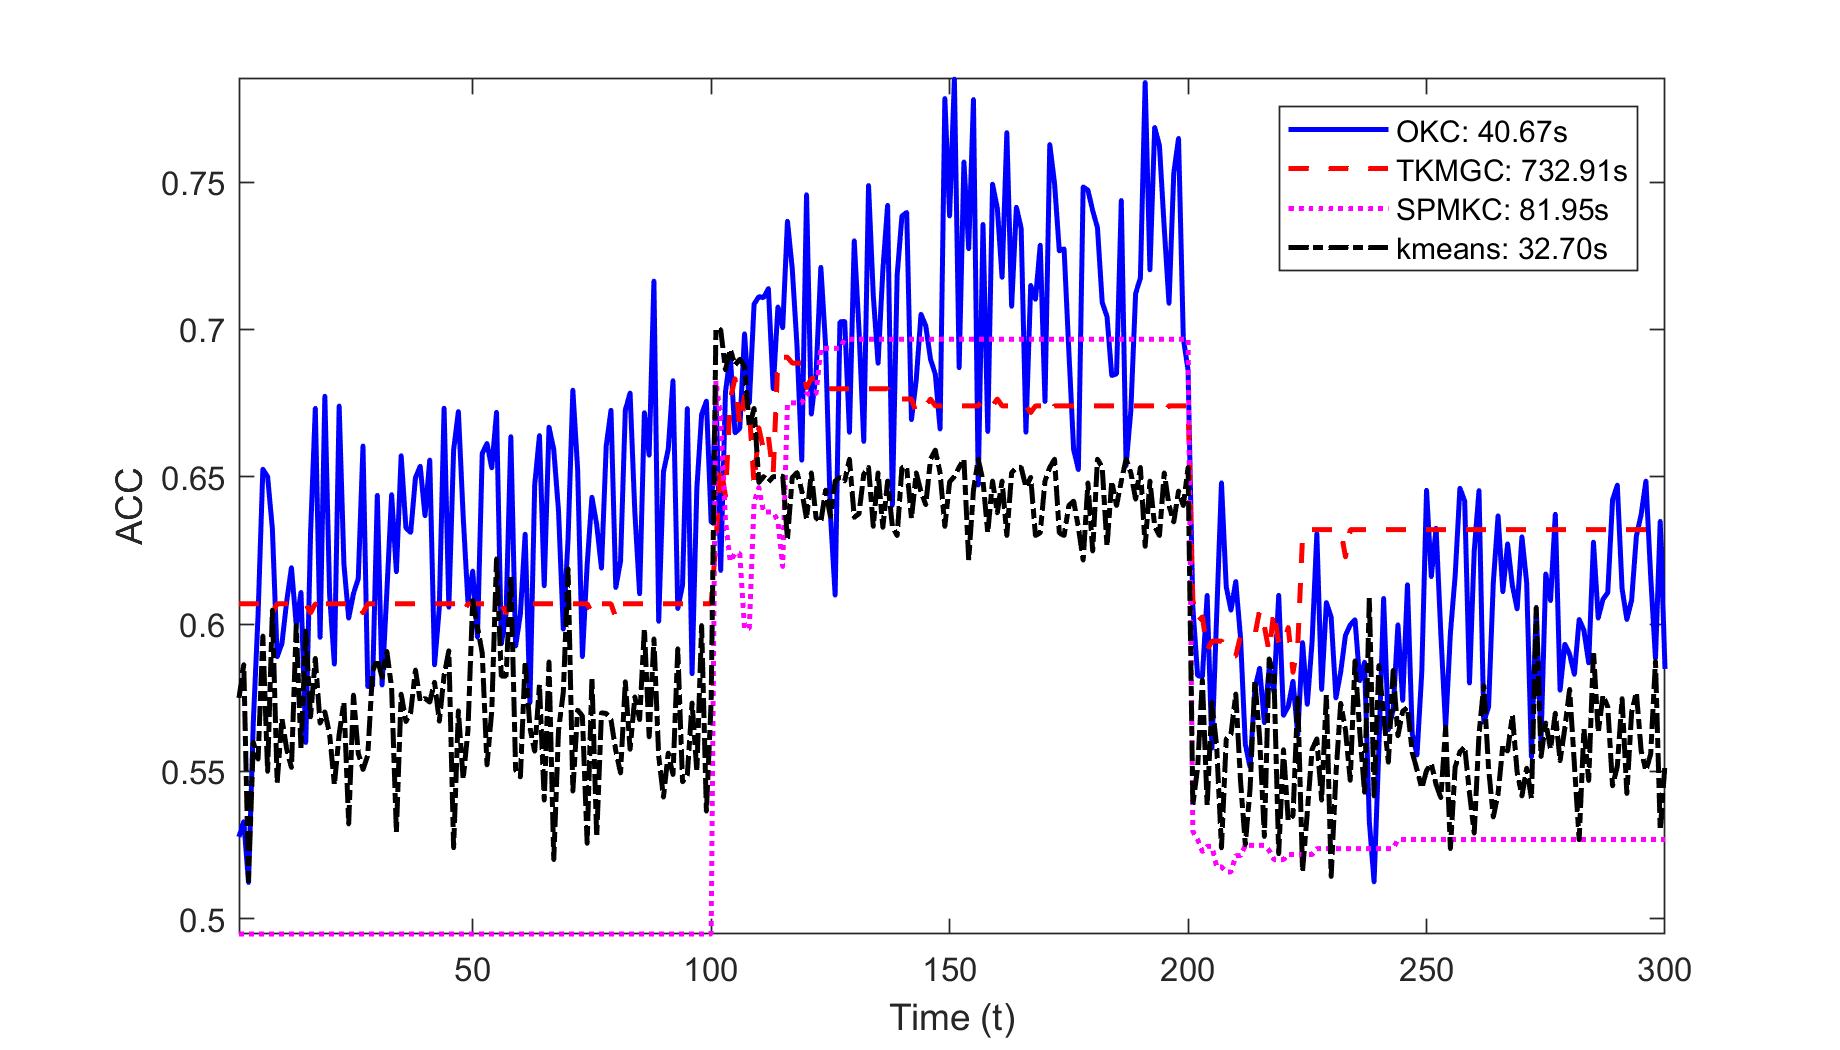
\includegraphics[scale=0.19]{avg_combined_ACC_plots_Unimib.png}
    \caption{Accuracy versus time in Unimib dataset.}
    \label{Fig:3u}
\end{figure}
%Although the simulation results displayed in table 1 were recorded from 3000 iterations, each plot shown in this section was generated across 300 iterations to maintain consistency with the TKMGC method due to its extended runtime. 
\begin{figure}[htp]
    \centering
    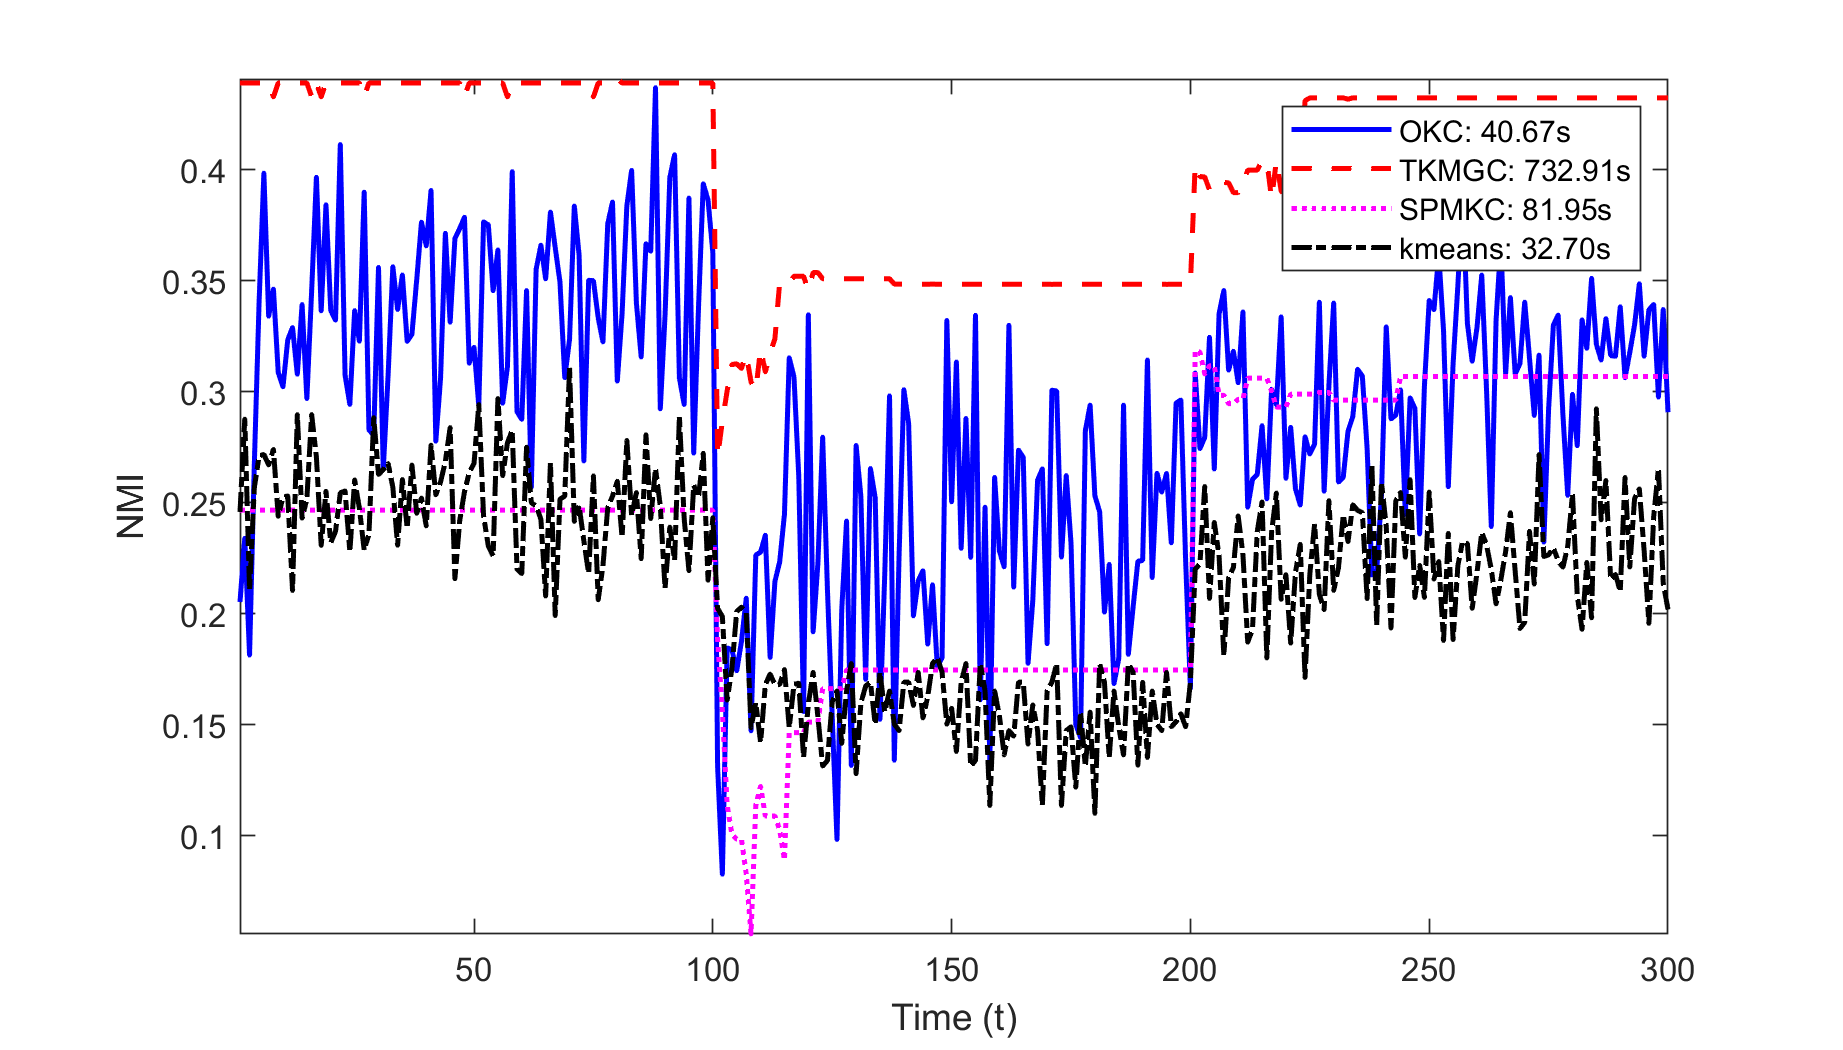
\includegraphics[scale=0.19]{avg_combined_NMI_plots_Unimib.png}
    \caption{NMI versus time in Unimib dataset.}
    \label{Fig:4u}
\end{figure}
Clearly, from Fig. \ref{Fig:4u} it can be seen that TKMGC exhibits lower accuracy, within time interval $[0,200]$, than the proposed OKC, but approximately the same maximum accuracy within time interval $[200,300]$. TKMGC exhibits slightly improved NMI and purity readings, however its runtime is almost 18 times that of the novel OKC algorithm. Detailed accuracy, NMI and purity measurements across $30$ independent trials achieved by TKMGC on the Unimib dataset are tabulated in Table II.
\begin{center}
\begin{table}[h!]
\begin{tabular}{|c|c|c|c|c|c|c|c|c|}
    \hline
    \multicolumn{3}{|c|}{0-100} & \multicolumn{3}{|c|}{101-200} & \multicolumn{3}{|c|}{201-300}\\
    \hline
    ACC & NMI & PUR & ACC & NMI & PUR & ACC & NMI & PUR\\
    \hline
    0.74 & 0.50 & 0.83 & 0.63 & 0.33 & 0.92 & 0.52 & 0.28 & 0.62\\
    0.49 & 0.23 & 0.60 & 0.63 & 0.20 & 0.85 & 0.60 & 0.30 & 0.70\\
    0.39 & 0.13 & 0.52 & 0.76 & 0.28 & 0.92 & 0.46 & 0.18 & 0.50\\
    0.72 & 0.66 & 0.92 & 0.79 & 0.46 & 0.94 & 0.73 & 0.53 & 0.79\\
    0.50 & 0.36 & 0.67 & 0.77 & 0.36 & 0.87 & 0.47 & 0.23 & 0.55\\
    0.62 & 0.45 & 0.77 & 0.68 & 0.31 & 0.83 & 0.64 & 0.51 & 0.77\\
    0.50 & 0.23 & 0.57 & 0.77 & 0.29 & 0.83 & 0.45 & 0.14 & 0.52\\
    0.75 & 0.53 & 0.85 & 0.65 & 0.38 & 0.90 & 0.63 & 0.48 & 0.71\\
    0.71 & 0.50 & 0.81 & 0.81 & 0.36 & 0.93 & 0.58 & 0.35 & 0.68\\
    0.50 & 0.24 & 0.58 & 0.56 & 0.09 & 0.77 & 0.46 & 0.13 & 0.54\\
    0.62 & 0.43 & 0.75 & 0.62 & 0.27 & 0.88 & 0.75 & 0.58 & 0.87\\
    0.44 & 0.14 & 0.51 & 0.60 & 0.05 & 0.69 & 0.45 & 0.23 & 0.55\\
    0.58 & 0.49 & 0.69 & 0.71 & 0.35 & 0.92 & 0.67 & 0.45 & 0.78\\
    0.49 & 0.43 & 0.63 & 0.58 & 0.22 & 0.76 & 0.64 & 0.37 & 0.71\\
    0.58 & 0.47 & 0.70 & 0.74 & 0.45 & 0.89 & 0.55 & 0.31 & 0.64\\
    0.62 & 0.44 & 0.77 & 0.71 & 0.37 & 0.86 & 0.46 & 0.27 & 0.61\\
    0.56 & 0.32 & 0.67 & 0.82 & 0.43 & 0.94 & 0.56 & 0.31 & 0.69\\
    0.74 & 0.60 & 0.90 & 0.67 & 0.33 & 0.91 & 0.57 & 0.34 & 0.69\\
    0.67 & 0.46 & 0.78 & 0.80 & 0.47 & 0.94 & 0.67 & 0.48 & 0.70\\
    0.55 & 0.24 & 0.67 & 0.67 & 0.17 & 0.78 & 0.54 & 0.27 & 0.63\\
    0.79 & 0.62 & 0.90 & 0.74 & 0.51 & 0.98 & 0.76 & 0.64 & 0.88\\
    0.67 & 0.45 & 0.77 & 0.76 & 0.46 & 0.95 & 0.60 & 0.36 & 0.67\\
    0.87 & 0.74 & 0.97 & 0.78 & 0.53 & 0.98 & 0.63 & 0.33 & 0.72\\
    0.79 & 0.64 & 0.89 & 0.80 & 0.61 & 1.00 & 0.67 & 0.50 & 0.74\\
    0.61 & 0.40 & 0.72 & 0.77 & 0.42 & 0.93 & 0.56 & 0.34 & 0.66\\
    0.65 & 0.52 & 0.79 & 0.53 & 0.25 & 0.83 & 0.42 & 0.16 & 0.53\\
    0.64 & 0.46 & 0.76 & 0.76 & 0.40 & 0.90 & 0.53 & 0.30 & 0.67\\
    0.65 & 0.46 & 0.78 & 0.67 & 0.39 & 0.92 & 0.59 & 0.35 & 0.67\\
    \hline
\end{tabular}
\caption{\label{tab:Table II}Accuracy, NMI, and Purity of TKMGC applied in Unimib dataset.}
\end{table}
\end{center}

\begin{figure}[htp]
    \centering
    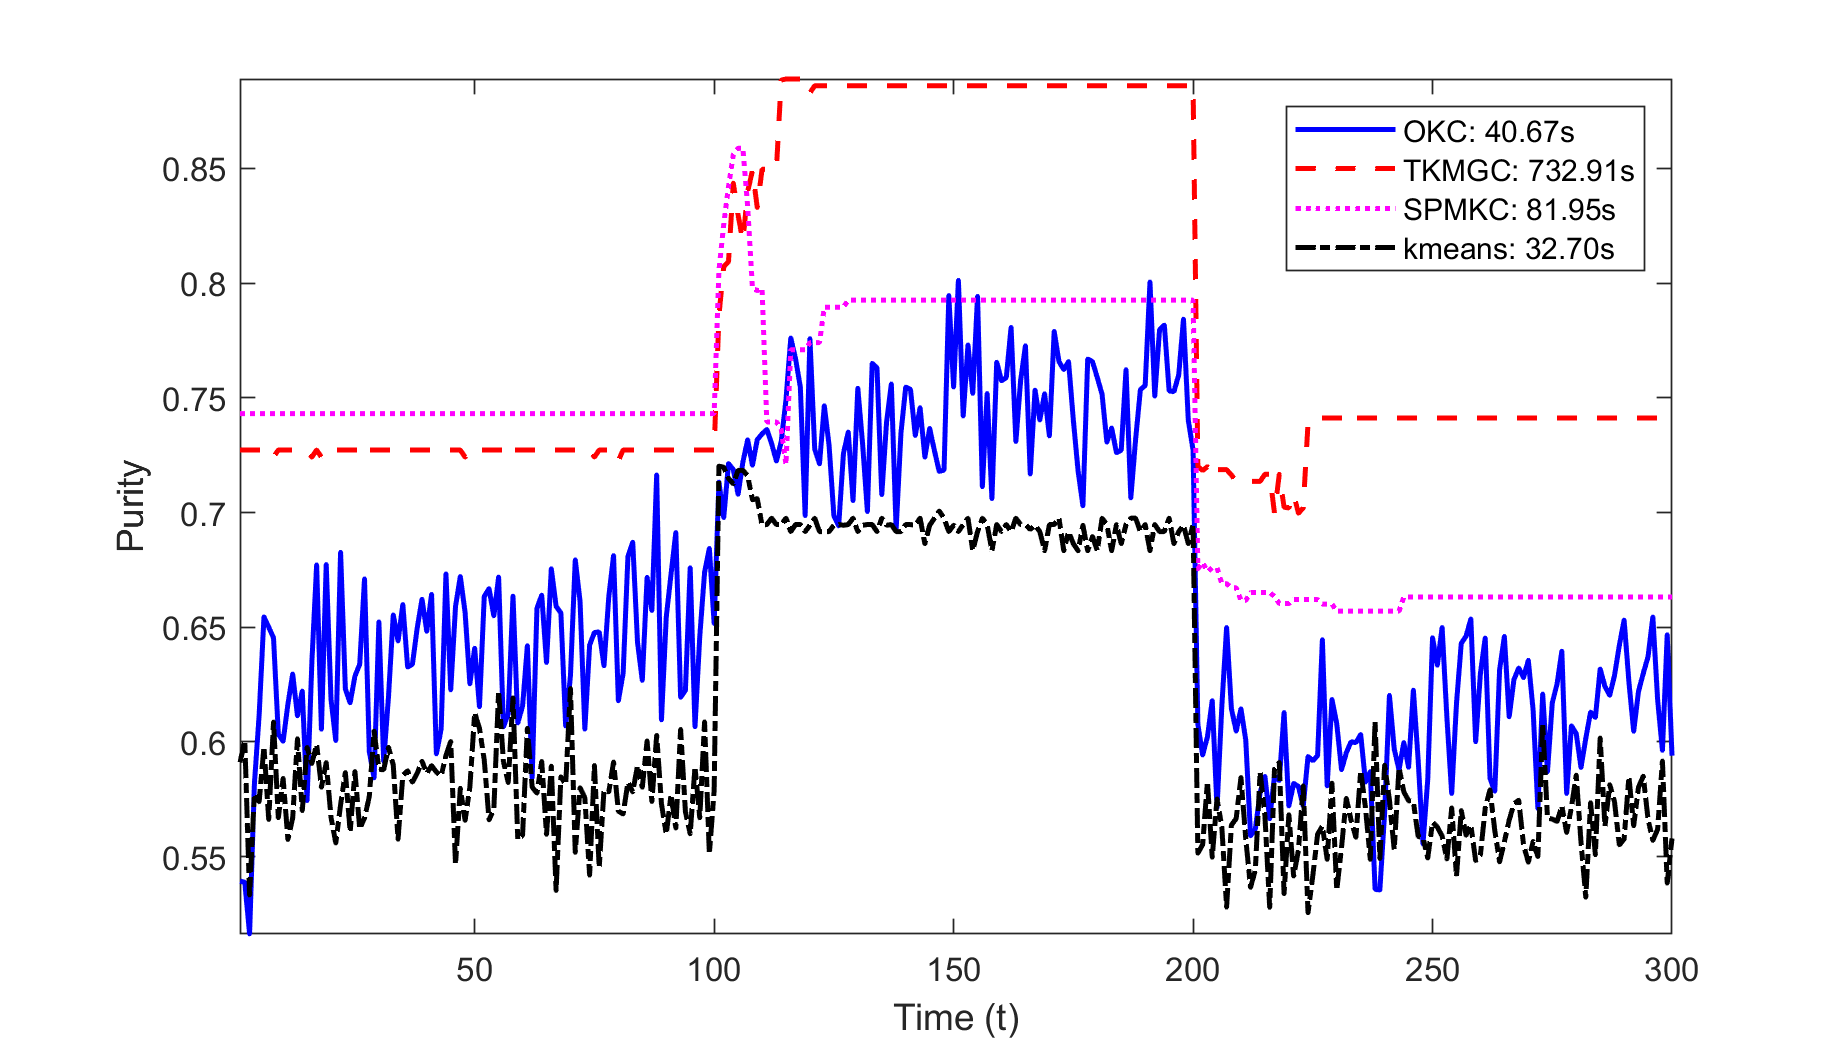
\includegraphics[scale=0.19]{avg_combined_Purity_plots_Unimib.png}
    \caption{Purity versus time in Unimib dataset.}
    \label{Fig:5u}
\end{figure}
Figs. \ref{Fig:3u}-\ref{Fig:5u} depicts that the SPMKC approach when applied on the Unimib dataset not only exhibits a lower accuracy across the entire time interval $[0,300]$, but also a lower NMI metric. Purity is slightly higher  than OKC, though runtime required by  SPMKC is about 2 times that of the OKC runtime. As in TKMGC, the results from applying SPMKC on Unimib is recorded in \textcolor{black}{{Table III}} over 30 independent trials.

\begin{center}
\begin{table}[h!]
\begin{tabular}{|c|c|c|c|c|c|c|c|c|}
    \hline
    \multicolumn{3}{|c|}{0-100} & \multicolumn{3}{|c|}{101-200} & \multicolumn{3}{|c|}{201-300}\\
    \hline
    ACC & NMI & PUR & ACC & NMI & PUR & ACC & NMI & PUR\\
    \hline
    0.71 & 0.41 & 0.71 & 0.70 & 0.16 & 0.82 & 0.74 & 0.48 & 0.74\\
    0.45 & 0.30 & 0.79 & 0.75 & 0.16 & 0.92 & 0.54 & 0.27 & 0.80\\
    0.46 & 0.15 & 0.61 & 0.77 & 0.20 & 0.94 & 0.46 & 0.20 & 0.83\\
    0.75 & 0.51 & 0.75 & 0.88 & 0.46 & 0.88 & 0.63 & 0.35 & 0.63\\
    0.50 & 0.33 & 0.63 & 0.82 & 0.30 & 0.85 & 0.53 & 0.31 & 0.68\\
    0.54 & 0.17 & 0.70 & 0.64 & 0.25 & 0.77 & 0.51 & 0.25 & 0.55\\
    0.60 & 0.24 & 0.68 & 0.82 & 0.30 & 0.93 & 0.40 & 0.07 & 0.67\\
    0.53 & 0.32 & 0.81 & 0.74 & 0.13 & 0.93 & 0.44 & 0.18 & 0.63\\
    0.58 & 0.35 & 0.78 & 0.89 & 0.46 & 0.89 & 0.64 & 0.38 & 0.67\\
    0.58 & 0.23 & 0.71 & 0.75 & 0.23 & 0.77 & 0.46 & 0.13 & 0.52\\
    0.47 & 0.34 & 0.80 & 0.83 & 0.35 & 0.88 & 0.67 & 0.44 & 0.70\\
    0.49 & 0.23 & 0.53 & 0.76 & 0.28 & 0.94 & 0.55 & 0.29 & 0.85\\
    0.50 & 0.25 & 0.61 & 0.72 & 0.11 & 0.72 & 0.54 & 0.29 & 0.57\\
    0.46 & 0.27 & 0.79 & 0.79 & 0.25 & 0.88 & 0.46 & 0.27 & 0.79\\
    0.53 & 0.23 & 0.69 & 0.58 & 0.05 & 0.92 & 0.55 & 0.49 & 0.82\\
    0.54 & 0.39 & 0.83 & 0.86 & 0.40 & 0.90 & 0.52 & 0.43 & 0.86\\
    0.41 & 0.17 & 0.85 & 0.82 & 0.30 & 0.93 & 0.50 & 0.32 & 0.82\\
    0.48 & 0.14 & 0.48 & 0.64 & 0.08 & 0.88 & 0.50 & 0.10 & 0.52\\
    0.59 & 0.26 & 0.70 & 0.82 & 0.43 & 0.94 & 0.57 & 0.25 & 0.65\\
    0.69 & 0.40 & 0.71 & 0.91 & 0.53 & 0.91 & 0.64 & 0.43 & 0.77\\
    0.60 & 0.58 & 0.93 & 0.93 & 0.66 & 0.93 & 0.69 & 0.41 & 0.81\\
    0.81 & 0.56 & 0.81 & 0.72 & 0.32 & 0.72 & 0.68 & 0.47 & 0.72\\
    0.40 & 0.15 & 0.87 & 0.67 & 0.27 & 0.67 & 0.53 & 0.39 & 0.77\\
    0.44 & 0.08 & 0.62 & 0.82 & 0.31 & 0.85 & 0.50 & 0.39 & 0.82\\
    0.48 & 0.27 & 0.63 & 0.70 & 0.10 & 0.70 & 0.47 & 0.30 & 0.67\\
    0.76 & 0.51 & 0.81 & 0.85 & 0.33 & 0.85 & 0.51 & 0.20 & 0.76\\
    0.48 & 0.30 & 0.81 & 0.87 & 0.51 & 0.87 & 0.75 & 0.44 & 0.75\\
    0.74 & 0.49 & 0.80 & 0.96 & 0.83 & 0.95 & 0.60 & 0.32 & 0.78\\
    \hline
\end{tabular}
\caption{\label{tab:Table III}Accuracy, NMI, and Purity of SPMKC applied in Unimib dataset.}
\end{table}
\end{center}

Figs. \ref{Fig:3u}-\ref{Fig:5u} show that K-means performs worse than OKC for approximately a similar runtime. K-means performed worse compared to  TKMGC and SPMKC in terms of the NMI and Purity metrics are well. Detailed accuracy, NMI and purity measurements across $30$ independent trials achieved by K-means on the Unimib dataset are tabulated in Table IV.

\begin{figure}[htp]
    \centering
    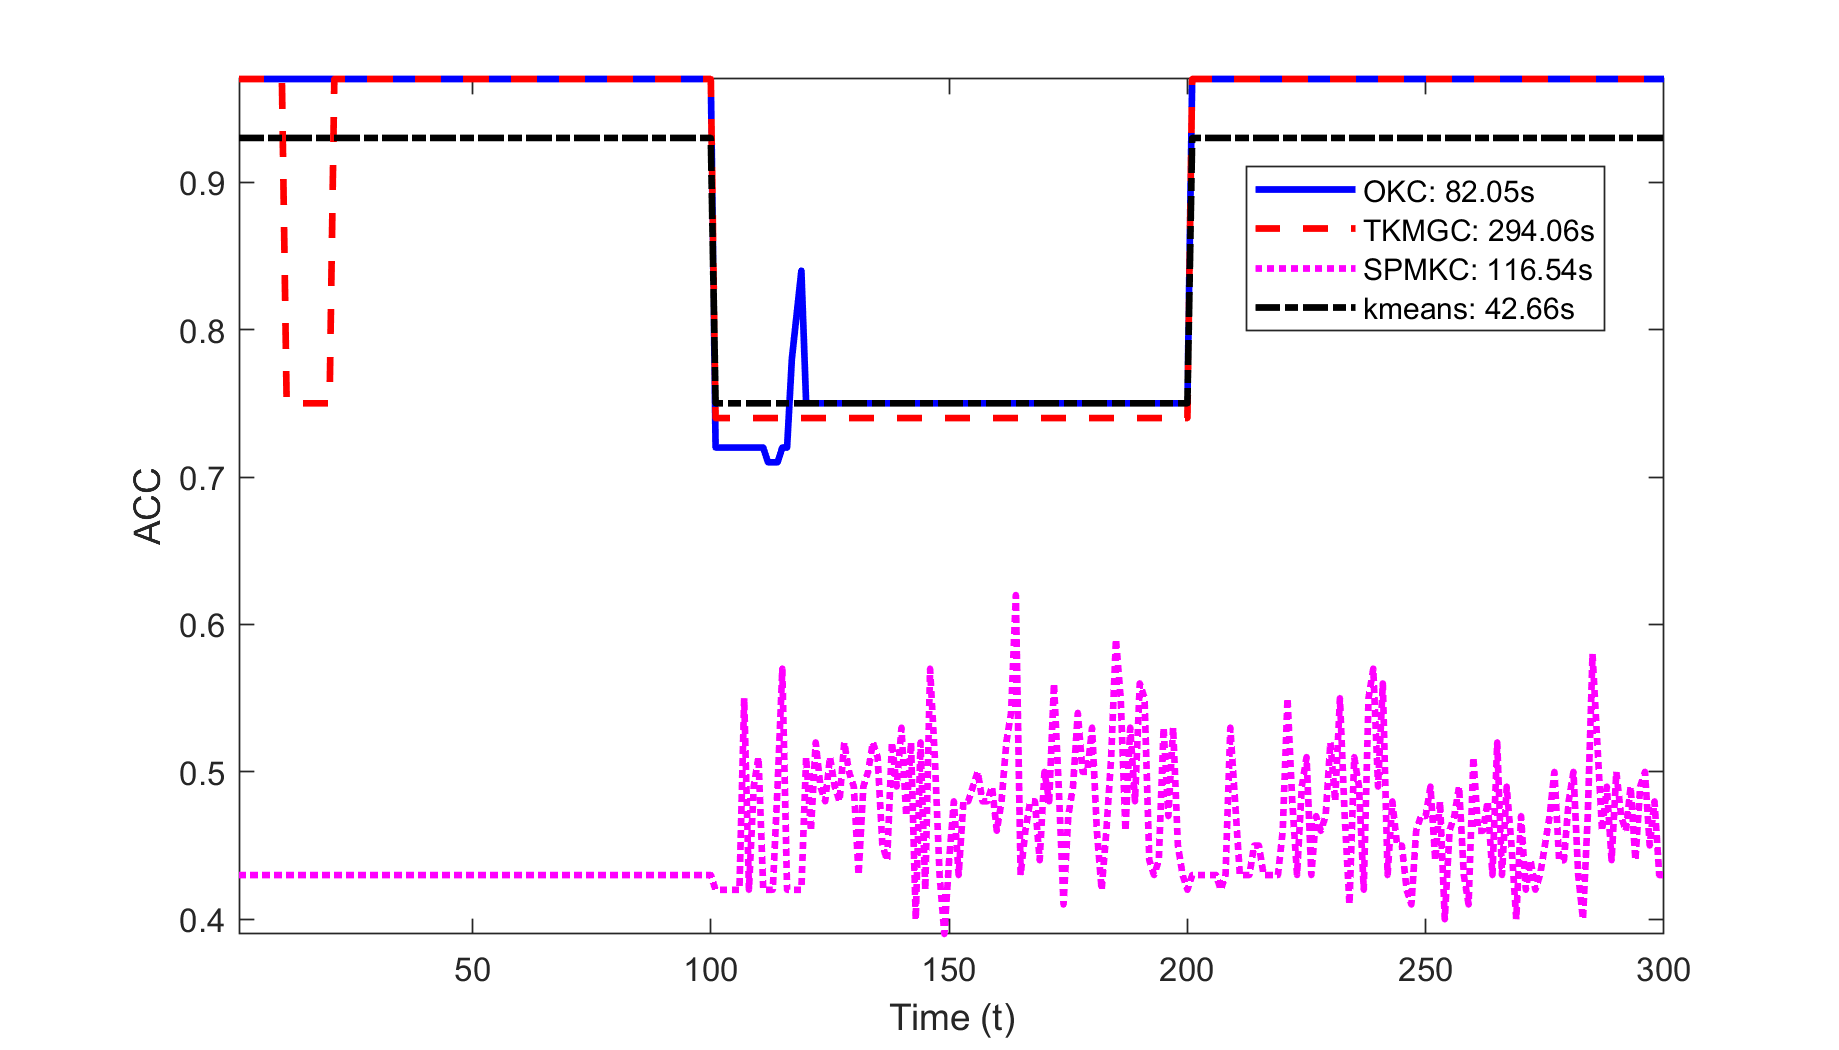
\includegraphics[scale=0.19]{avg_combined_ACC_plots_Salinas.png}
    \caption{Accuracy vs time in Salinas dataset.}
    \label{Fig:4}
\end{figure}
\begin{center}
\begin{table}
\begin{tabular}{|c|c|c|c|c|c|c|c|c|}
    \hline
    \multicolumn{3}{|c|}{0-100} & \multicolumn{3}{|c|}{101-200} & \multicolumn{3}{|c|}{201-300}\\
    \hline
    ACC & NMI & Purity & ACC & NMI & Purity & ACC & NMI & Purity\\
    \hline
    0.80 & 0.55 & 0.80 & 0.68 & 0.28 & 0.68 & 0.76 & 0.48 & 0.76\\
    0.73 & 0.46 & 0.73 & 0.58 & 0.06 & 0.67 & 0.80 & 0.46 & 0.80\\
    0.53 & 0.20 & 0.53 & 0.62 & 0.02 & 0.67 & 0.53 & 0.23 & 0.53\\
    0.63 & 0.34 & 0.63 & 0.56 & 0.00 & 0.67 & 0.60 & 0.30 & 0.60\\
    0.85 & 0.59 & 0.85 & 0.73 & 0.29 & 0.73 & 0.63 & 0.39 & 0.63\\
    0.66 & 0.46 & 0.66 & 0.64 & 0.25 & 0.67 & 0.66 & 0.35 & 0.66\\
    0.57 & 0.26 & 0.57 & 0.62 & 0.05 & 0.67 & 0.48 & 0.13 & 0.48\\
    0.79 & 0.55 & 0.79 & 0.65 & 0.20 & 0.67 & 0.67 & 0.42 & 0.67\\
    0.83 & 0.68 & 0.83 & 0.67 & 0.14 & 0.67 & 0.67 & 0.42 & 0.67\\
    0.60 & 0.26 & 0.60 & 0.73 & 0.12 & 0.73 & 0.60 & 0.22 & 0.60\\
    0.73 & 0.46 & 0.73 & 0.83 & 0.30 & 0.83 & 0.80 & 0.58 & 0.89\\
    0.66 & 0.30 & 0.65 & 0.65 & 0.25 & 0.67 & 0.60 & 0.30 & 0.60\\
    0.67 & 0.43 & 0.67 & 0.57 & 0.02 & 0.67 & 0.54 & 0.29 & 0.54\\
    0.68 & 0.48 & 0.68 & 0.65 & 0.26 & 0.67 & 0.67 & 0.44 & 0.67\\
    0.67 & 0.36 & 0.67 & 0.55 & 0.02 & 0.67 & 0.59 & 0.33 & 0.59\\
    0.71 & 0.49 & 0.70 & 0.69 & 0.29 & 0.69 & 0.60 & 0.31 & 0.62\\
    0.69 & 0.38 & 0.69 & 0.78 & 0.32 & 0.78 & 0.78 & 0.50 & 0.78\\
    0.60 & 0.31 & 0.60 & 0.62 & 0.03 & 0.67 & 0.64 & 0.41 & 0.64\\
    0.69 & 0.45 & 0.69 & 0.70 & 0.31 & 0.70 & 0.69 & 0.36 & 0.69\\
    0.63 & 0.34 & 0.63 & 0.73 & 0.23 & 0.73 & 0.59 & 0.32 & 0.59\\
    0.67 & 0.31 & 0.67 & 0.64 & 0.09 & 0.67 & 0.57 & 0.27 & 0.57\\
    0.82 & 0.60 & 0.82 & 0.72 & 0.32 & 0.72 & 0.64 & 0.32 & 0.64\\
    0.78 & 0.58 & 0.78 & 0.77 & 0.37 & 0.77 & 0.77 & 0.50 & 0.77\\
    0.56 & 0.29 & 0.56 & 0.62 & 0.03 & 0.67 & 0.59 & 0.30 & 0.59\\
    0.54 & 0.21 & 0.54 & 0.53 & 0.01 & 0.67 & 0.56 & 0.20 & 0.56\\
    0.86 & 0.71 & 0.86 & 0.67 & 0.27 & 0.67 & 0.60 & 0.23 & 0.60\\
    0.68 & 0.48 & 0.68 & 0.66 & 0.26 & 0.67 & 0.70 & 0.42 & 0.70\\
    0.77 & 0.44 & 0.77 & 0.67 & 0.27 & 0.67 & 0.65 & 0.44 & 0.65\\
    \hline
\end{tabular}
\caption{\label{tab: Table IV}Accuracy, NMI, and Purity of Kmeans applied in Unimib dataset.}
\end{table}
\end{center}

Figs. \ref{Fig:4}-\ref{Fig:6} were obtained after testing the accuracy, NMI and purity of OKC, SPMKC and TMKGC on the Salinas dataset. %As in Unimib, these sets of plots were produced across 300 iterations as TKMGC performs much slower than TKMGC Unimib. 
\begin{figure}[htp]
    \centering
    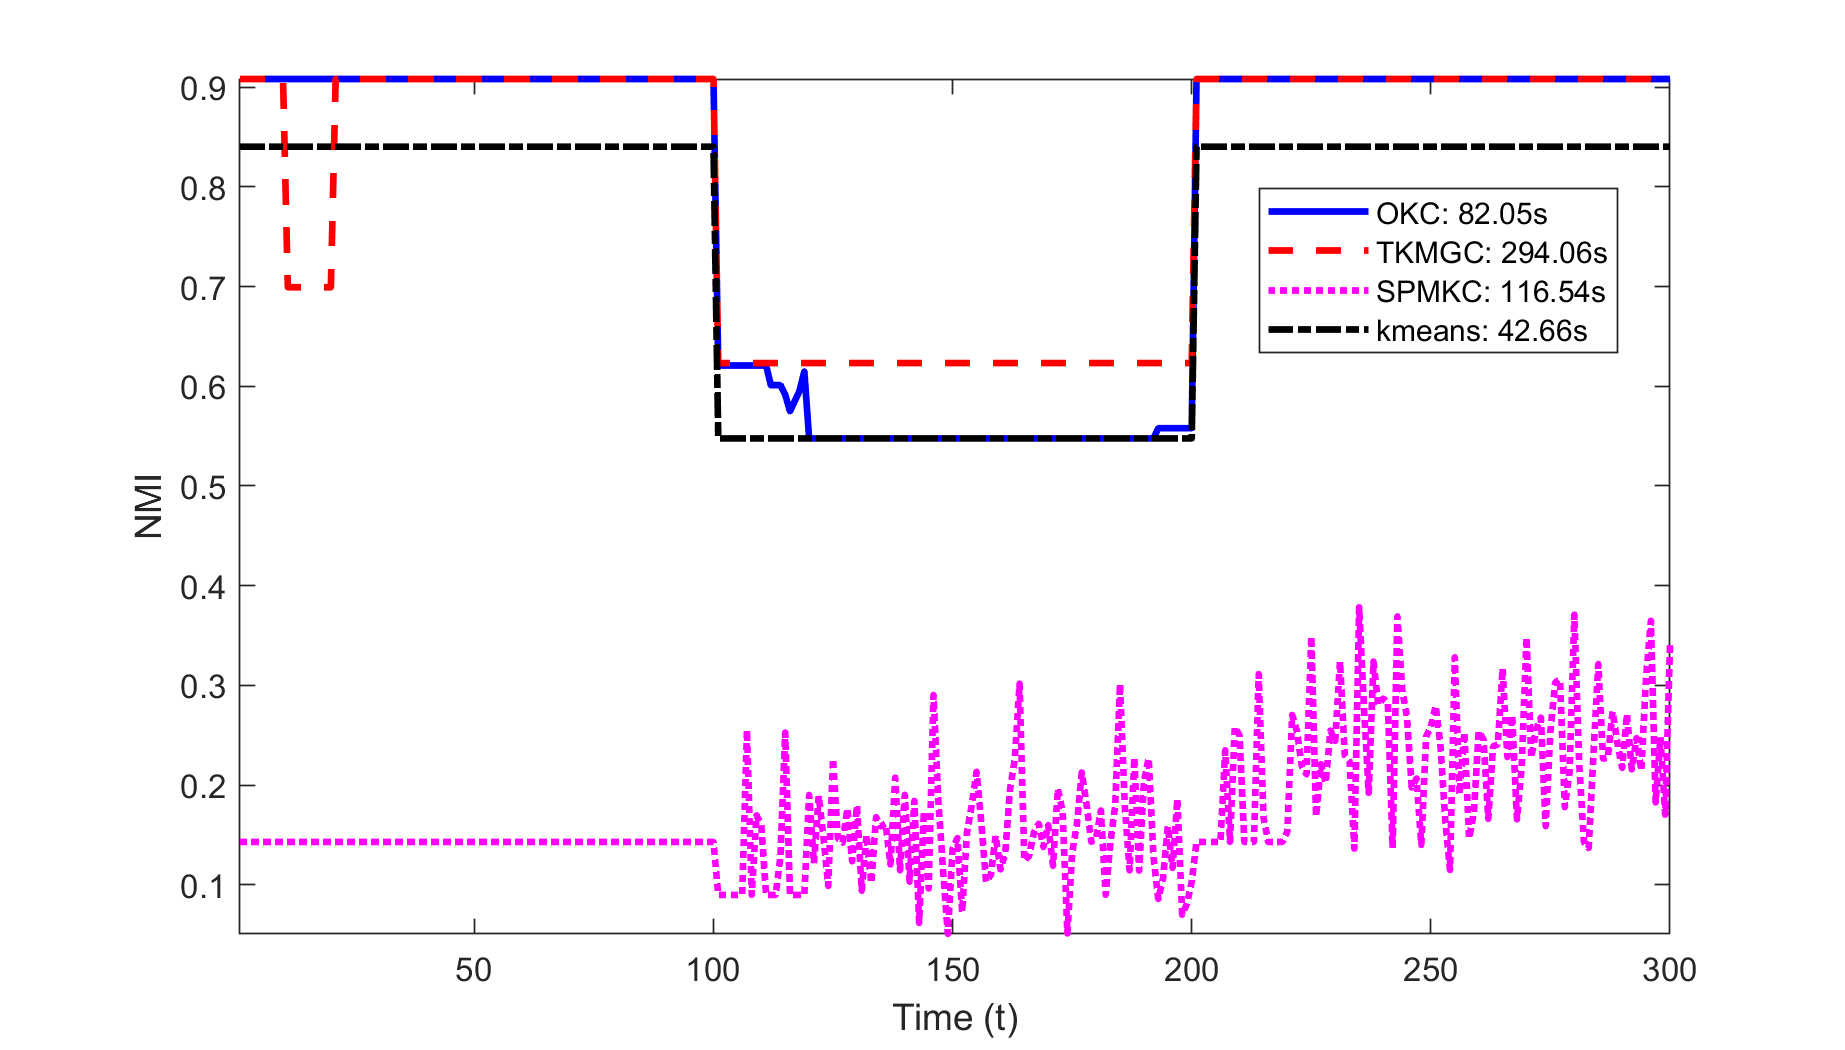
\includegraphics[scale=0.19]{avg_combined_NMI_plots_Salinas.png}
    \caption{NMI vs time in Salinas dataset.}
    \label{Fig:5}
\end{figure}
OKC method demonstrates high accuracy, NMI, and purity within the time intervals $[0,100]$ as well as $[200,300]$. The drop in accuracy, NMI and Purity in OKC can be attributed to the change in the number of classes, \begin{math}Q\end{math}, from 4 to 3 within $[100,200]$ and then back to 4  within $[200,300]$.
\begin{figure}[htp]
    \centering
    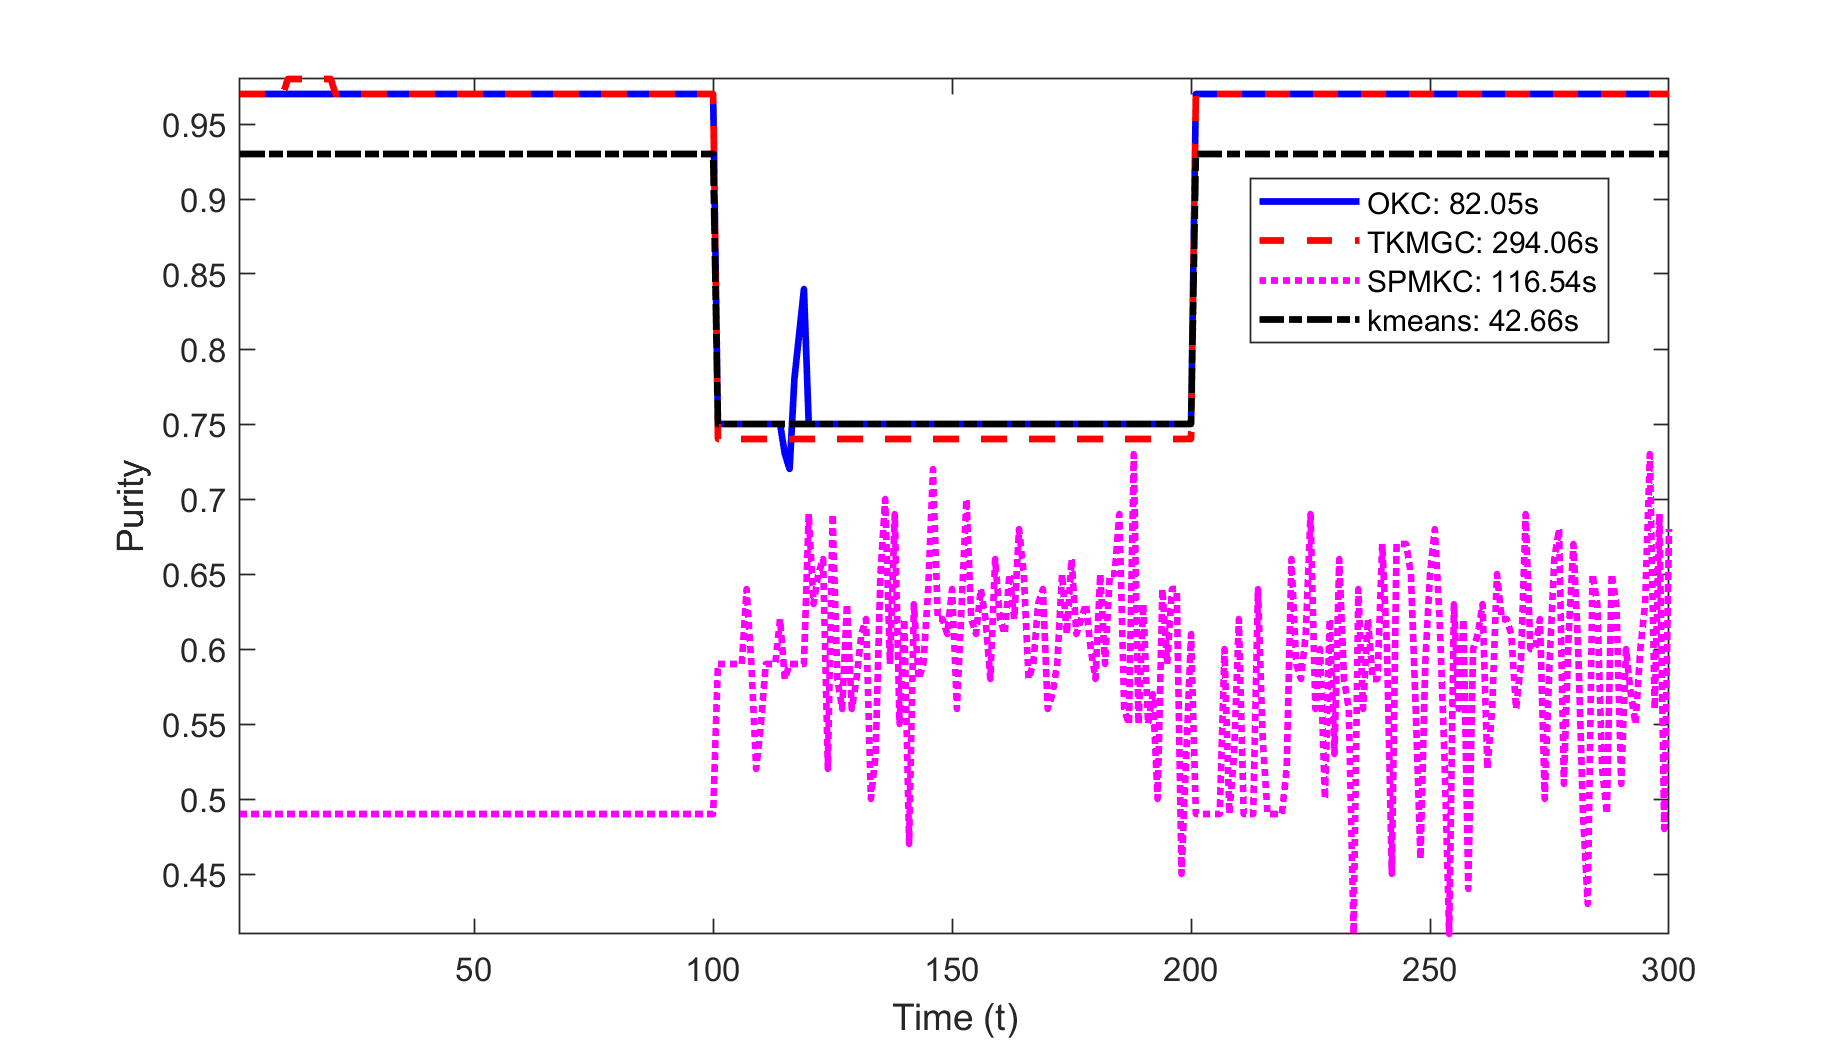
\includegraphics[scale=0.19]{avg_combined_Purity_plots_Salinas.png}
    \caption{Purity vs time in Salinas dataset.}
    \label{Fig:6}
\end{figure}
Figs. \ref{Fig:4}-\ref{Fig:6} show that OKC and  TKMGC perform similarly, while the remaining method are worse with respect to all three different metrics examined. Though, again the advantage of OKC over TMKGC is the significantly lower running time required as reported in the legends of Figs. \ref{Fig:4}-\ref{Fig:6}. The overall accuracy of TKMGC Salinas is only about 3\% better than the proposed method, however its runtime was about 294 seconds, whereas that of OKC was approximately 69 seconds. %Therefore, a trade-off between accuracy and runtime can be considered as the algorithm with the slightly improved results took about 4 times as much time to finish compilation.
%\begin{tabular}{|c|c|c|c|c|c|c|c|c|}
%    \hline
%    \multicolumn{3}{|c|}{0-100} & \multicolumn{3}{|c|}{101-200} & \multicolumn{3}{|c|}{201-300}\\
%    \hline
%    ACC & NMI & Purity & ACC & NMI & Purity & ACC & NMI & Purity\\
%    \hline
%    0.68 & 0.73 & 0.75 & 0.75 & 0.67 & 0.75 & 0.68 & 0.73 & 0.75\\
%    0.96 & 0.89 & 0.96 & 0.74 & 0.63 & 0.74 & 0.96 & 0.89 & 0.96\\
%    0.90 & 0.82 & 0.90 & 0.73 & 0.60 & 0.73 & 0.90 & 0.82 & 0.90\\
%    0.90 & 0.78 & 0.90 & 0.72 & 0.51 & 0.73 & 0.90 & 0.78 & 0.90\\
%    1.00 & 1.00 & 1.00 & 0.75 & 0.67 & 0.75 & 1.00 & 1.00 & 1.00\\
%    0.89 & 0.84 & 0.89 & 0.50 & 0.67 & 0.75 & 0.89 & 0.84 & 0.89\\
%    0.99 & 0.97 & 0.99 & 0.73 & 0.61 & 0.75 & 0.99 & 0.97 & 0.99\\
%    0.90 & 0.83 & 0.90 & 0.50 & 0.67 & 0.75 & 0.90 & 0.83 & 0.90\\
%    1.00 & 1.00 & 1.00 & 0.75 & 0.67 & 0.75 & 1.00 & 1.00 & 1.00\\
%    0.85 & 0.81 & 0.85 & 0.50 & 0.67 & 0.75 & 0.85 & 0.81 & 0.85\\
%    1.00 & 1.00 & 1.00 & 0.50 & 0.67 & 0.75 & 1.00 & 1.00 & 1.00\\
%    1.00 & 1.00 & 1.00 & 1.00 & 1.00 & 1.00 & 1.00 & 1.00 & 1.00\\
%    0.87 & 0.74 & 0.87 & 0.76 & 0.51 & 0.76 & 0.87 & 0.74 & 0.87\\
%    0.82 & 0.71 & 0.82 & 0.50 & 0.61 & 0.75 & 0.82 & 0.71 & 0.82\\
%    0.97 & 0.92 & 0.97 & 0.75 & 0.67 & 0.75 & 0.97 & 0.92 & 0.97\\
%    0.99 & 0.97 & 0.99 & 0.50 & 0.67 & 0.75 & 0.99 & 0.97 & 0.99\\
%    1.00 & 1.00 & 1.00 & 0.80 & 0.69 & 0.80 & 1.00 & 1.00 & 1.00\\
%    0.69 & 0.62 & 0.69 & 0.69 & 0.49 & 0.72 & 0.69 & 0.62 & 0.69\\
%    0.99 & 0.97 & 0.99 & 0.50 & 0.67 & 0.75 & 0.99 & 0.97 & 0.99\\
%    0.95 & 0.87 & 0.95 & 0.55 & 0.52 & 0.73 & 0.95 & 0.87 & 0.95\\
%    0.99 & 0.97 & 0.99 & 0.74 & 0.62 & 0.74 & 0.99 & 0.97 & 0.99\\
%    1.00 & 1.00 & 1.00 & 0.75 & 0.67 & 0.75 & 1.00 & 1.00 & 1.00\\
%    0.77 & 0.64 & 0.77 & 0.73 & 0.63 & 0.75 & 0.77 & 0.64 & 0.77\\
%    0.67 & 0.57 & 0.67 & 0.54 & 0.28 & 0.54 & 0.67 & 0.57 & 0.67\\
%    0.99 & 0.97 & 0.99 & 0.99 & 0.95 & 0.99 & 0.99 & 0.97 & 0.99\\
%    0.99 & 0.97 & 0.99 & 0.74 & 0.63 & 0.74 & 0.99 & 0.97 & 0.99\\
%    0.66 & 0.65 & 0.72 & 0.71 & 0.52 & 0.72 & 0.66 & 0.65 & 0.72\\
%    1.00 & 1.00 & 1.00 & 1.00 & 1.00 & 1.00 & 1.00 & 1.00 & 1.00\\
%    0.94 & 0.89 & 0.94 & 0.75 & 0.55 & 0.75 & 0.94 & 0.89 & 0.94\\
%    0.93 & 0.83 & 0.93 & 0.68 & 0.43 & 0.72 & 0.93 & 0.83 & 0.93\\
%    0.91 & 0.78 & 0.91 & 0.67 & 0.47 & 0.74 & 0.91 & 0.78 & 0.91\\
%    0.95 & 0.88 & 0.95 & 0.75 & 0.67 & 0.75 & 0.95 & 0.88 & 0.95\\
%    1.00 & 1.00 & 1.00 & 0.74 & 0.63 & 0.75 & 1.00 & 1.00 & 1.00\\
%    0.91 & 0.84 & 0.91 & 0.99 & 0.96 & 0.99 & 0.91 & 0.84 & 0.91\\
%    0.86 & 0.74 & 0.86 & 0.67 & 0.50 & 0.74 & 0.86 & 0.74 & 0.86\\
%    0.98 & 0.95 & 0.98 & 0.73 & 0.60 & 0.73 & 0.98 & 0.95 & 0.98\\
%    0.99 & 0.97 & 0.99 & 0.74 & 0.62 & 0.74 & 0.99 & 0.97 & 0.99\\
%    0.90 & 0.76 & 0.90 & 0.71 & 0.49 & 0.71 & 0.90 & 0.76 & 0.90\\
%    0.63 & 0.59 & 0.68 & 0.73 & 0.56 & 0.73 & 0.63 & 0.59 & 0.63\\
%    0.95 & 0.90 & 0.95 & 0.84 & 0.64 & 0.84 & 0.95 & 0.90 & 0.95\\
%    0.64 & 0.70 & 0.70 & 0.54 & 0.67 & 0.75 & 0.64 & 0.61 & 0.70\\
%    0.90 & 0.83 & 0.90 & 1.00 & 1.00 & 1.00 & 0.90 & 0.83 & 0.90\\
%    0.97 & 0.93 & 0.97 & 0.75 & 0.67 & 0.75 & 0.97 & 0.93 & 0.97\\
%    0.76 & 0.69 & 0.76 & 0.53 & 0.53 & 0.75 & 0.76 & 0.69 & 0.76\\
%    0.95 & 0.87 & 0.95 & 0.77 & 0.64 & 0.77 & 0.95 & 0.87 & 0.95\\
%    0.99 & 0.97 & 0.99 & 0.74 & 0.63 & 0.74 & 0.99 & 0.97 & 0.99\\
%    1.00 & 1.00 & 1.00 & 0.75 & 0.67 & 0.75 & 1.00 & 1.00 & 1.00\\
%    0.97 & 0.91 & 0.97 & 0.69 & 0.47 & 0.73 & 0.97 & 0.91 & 0.97\\
%    0.91 & 0.82 & 0.91 & 0.66 & 0.60 & 0.75 & 0.91 & 0.59 & 0.91\\
%    0.75 & 0.68 & 0.75 & 0.74 & 0.55 & 0.74 & 0.75 & 0.68 & 0.75\\
%    0.97 & 0.91 & 0.97 & 0.75 & 0.55 & 0.75 & 0.97 & 0.91 & 0.97\\
%    0.99 & 0.97 & 0.99 & 0.75 & 0.67 & 0.75 & 0.99 & 0.97 & 0.99\\
%    0.99 & 0.97 & 0.99 & 0.75 & 0.67 & 0.75 & 0.99 & 0.97 & 0.99\\
%    0.99 & 0.97 & 0.99 & 1.00 & 1.00 & 1.00 & 0.99 & 0.97 & 0.99\\
%    0.79 & 0.75 & 0.79 & 0.50 & 0.67 & 0.75 & 0.79 & 0.75 & 0.79\\
%    0.77 & 0.69 & 0.77 & 0.54 & 0.61 & 0.75 & 0.77 & 0.69 & 0.77\\
%    0.87 & 0.79 & 0.87 & 0.75 & 0.67 & 0.75 & 0.87 & 0.79 & 0.97\\
%    0.98 & 0.95 & 0.98 & 0.72 & 0.59 & 0.75 & 0.98 & 0.95 & 0.98\\
%    0.98 & 0.95 & 0.98 & 0.94 & 0.83 & 0.94 & 0.98 & 0.95 & 0.98\\
%    1.00 & 1.00 & 1.00 & 0.75 & 0.67 & 0.75 & 1.00 & 1.00 & 1.00\\
%    0.94 & 0.86 & 0.94 & 0.76 & 0.67 & 0.76 & 0.94 & 0.86 & 0.94\\
%    0.98 & 0.95 & 0.98 & 0.75 & 0.67 & 0.75 & 0.98 & 0.95 & 0.98\\
%    0.89 & 0.84 & 0.89 & 0.75 & 0.67 & 0.75 & 0.89 & 0.84 & 0.89\\
%    0.99 & 0.97 & 0.99 & 0.75 & 0.67 & 0.75 & 0.99 & 0.97 & 0.99\\
%    1.00 & 1.00 & 1.00 & 0.50 & 0.67 & 0.75 & 1.00 & 1.00 & 1.00\\
%    0.92 & 0.87 & 0.92 & 0.75 & 0.67 & 0.75 & 0.92 & 0.87 & 0.92\\
%    0.95 & 0.89 & 0.95 & 0.70 & 0.56 & 0.75 & 0.95 & 0.89 & 0.95\\
%    0.95 & 0.89 & 0.95 & 0.71 & 0.57 & 0.75 & 0.95 & 0.89 & 0.95\\
%    0.99 & 0.97 & 0.99 & 0.74 & 0.62 & 0.74 & 0.99 & 0.97 & 0.99\\
%    0.79 & 0.70 & 0.79 & 0.69 & 0.58 & 0.75 & 0.79 & 0.70 & 0.79\\
%    0.94 & 0.85 & 0.94 & 0.69 & 0.37 & 0.69 & 0.94 & 0.85 & 0.94\\
%    0.98 & 0.95 & 0.98 & 0.75 & 0.61 & 0.75 & 0.98 & 0.95 & 0.98\\
%    0.88 & 0.83 & 0.88 & 0.74 & 0.63 & 0.75 & 0.88 & 0.83 & 0.88\\
%    0.98 & 0.95 & 0.98 & 0.75 & 0.67 & 0.75 & 0.98 & 0.95 & 0.98\\
%    0.96 & 0.89 & 0.96 & 0.56 & 0.54 & 0.75 & 0.96 & 0.89 & 0.96\\
%    1.00 & 1.00 & 1.00 & 0.75 & 0.67 & 0.75 & 1.00 & 1.00 & 1.00\\
%    0.86 & 0.82 & 0.86 & 0.60 & 0.52 & 0.75 & 0.86 & 0.82 & 0.86\\
%    0.92 & 0.84 & 0.92 & 0.66 & 0.39 & 0.66 & 0.92 & 0.84 & 0.92\\
%    1.00 & 1.00 & 1.00 & 0.75 & 0.67 & 0.75 & 1.00 & 1.00 & 1.00\\
%    0.85 & 0.77 & 0.85 & 0.50 & 0.67 & 0.75 & 0.85 & 0.77 & 0.85\\
%    0.93 & 0.84 & 0.93 & 0.53 & 0.57 & 0.75 & 0.93 & 0.84 & 0.93\\
%    0.96 & 0.90 & 0.96 & 0.52 & 0.57 & 0.75 & 0.96 & 0.90 & 0.96\\ 
%    1.00 & 1.00 & 1.00 & 0.75 & 0.61 & 0.75 & 1.00 & 1.00 & 1.00\\
%    0.92 & 0.81 & 0.92 & 0.89 & 0.70 & 0.89 & 0.92 & 0.81 & 0.92\\
%    1.00 & 1.00 & 1.00 & 0.75 & 0.67 & 0.75 & 1.00 & 1.00 & 1.00\\
%    0.99 & 0.97 & 0.99 & 0.76 & 0.67 & 0.76 & 0.99 & 0.97 & 0.99\\
%    1.00 & 1.00 & 1.00 & 0.75 & 0.67 & 0.75 & 1.00 & 1.00 & 1.00\\
%    1.00 & 1.00 & 1.00 & 0.75 & 0.67 & 0.75 & 1.00 & 1.00 & 1.00\\
%    0.80 & 0.68 & 0.80 & 0.63 & 0.40 & 0.73 & 0.80 & 0.68 & 0.80\\
%    0.99 & 0.97 & 0.99 & 0.76 & 0.67 & 0.76 & 0.99 & 0.97 & 0.99\\
%    1.00 & 1.00 & 1.00 & 0.75 & 0.67 & 0.75 & 1.00 & 1.00 & 1.00\\
%    0.99 & 0.97 & 0.99 & 0.84 & 0.71 & 0.84 & 0.99 & 0.97 & 0.99\\
%    0.64 & 0.66 & 0.75 & 0.67 & 0.53 & 0.75 & 0.64 & 0.66 & 0.75\\
%    0.93 & 0.83 & 0.93 & 0.51 & 0.47 & 0.71 & 0.93 & 0.83 & 0.93\\
%    0.99 & 0.97 & 0.99 & 0.75 & 0.67 & 0.75 & 0.99 & 0.97 & 0.99\\
%    1.00 & 1.00 & 1.00 & 0.74 & 0.66 & 0.75 & 1.00 & 1.00 & 1.00\\
%    0.98 & 0.94 & 0.98 & 0.74 & 0.63 & 0.75 & 0.98 & 0.94 & 0.98\\
%    0.96 & 0.90 & 0.96 & 0.69 & 0.55 & 0.75 & 0.96 & 0.90 & 0.96\\
%    0.98 & 0.95 & 0.98 & 0.73 & 0.60 & 0.73 & 0.98 & 0.95 & 0.98\\
%    0.99 & 0.97 & 0.99 & 0.51 & 0.63 & 0.75 & 0.99 & 0.97 & 0.99\\
%    \hline
%\end{tabular}
It can also be inferred that the accuracy, NMI, and purity achieved by SPMKC on the Salinas dataset is lower than both TKMGC Salinas and OKC methods, but it has a faster runtime than TKMGC. 
%\begin{tabular}{|c|c|c|c|c|c|c|c|c|}
%    \hline
%    \multicolumn{3}{|c|}{0-100} & \multicolumn{3}{|c|}{101-200} & \multicolumn{3}{|c|}{201-300}\\
%    \hline
%    ACC & NMI & PUR & ACC & NMI & PUR & ACC & NMI & PUR\\
%    \hline
%    0.50 & 0.51 & 0.75 & 0.57 & 0.32 & 0.76 & 0.50 & 0.51 & 0.75\\
%    0.38 & 0.33 & 0.77 & 0.54 & 0.21 & 0.76 & 0.51 & 0.37 & 0.78\\
%    0.49 & 0.21 & 0.57 & 0.56 & 0.27 & 0.76 & 0.55 & 0.36 & 0.69\\
%    0.46 & 0.12 & 0.49 & 0.56 & 0.18 & 0.69 & 0.49 & 0.25 & 0.57\\
%    0.54 & 0.33 & 0.55 & 0.68 & 0.43 & 0.71 & 0.59 & 0.34 & 0.59\\
%    0.47 & 0.38 & 0.82 & 0.54 & 0.27 & 0.75 & 0.50 & 0.42 & 0.85\\
%    0.48 & 0.27 & 0.52 & 0.69 & 0.40 & 0.80 & 0.55 & 0.31 & 0.58\\
%    0.38 & 0.09 & 0.52 & 0.51 & 0.27 & 0.68 & 0.48 & 0.23 & 0.61\\
%    0.36 & 0.39 & 0.84 & 0.42 & 0.21 & 0.75 & 0.50 & 0.45 & 0.87\\
%    0.42 & 0.11 & 0.43 & 0.50 & 0.16 & 0.74 & 0.51 & 0.26 & 0.66\\
%    0.60 & 0.33 & 0.60 & 0.80 & 0.50 & 0.80 & 0.62 & 0.38 & 0.64\\
%    0.55 & 0.40 & 0.70 & 0.78 & 0.50 & 0.87 & 0.59 & 0.45 & 0.75\\
%    0.44 & 0.23 & 0.61 & 0.62 & 0.29 & 0.76 & 0.51 & 0.32 & 0.68\\
%    0.44 & 0.21 & 0.55 & 0.50 & 0.19 & 0.77 & 0.48 & 0.31 & 0.81\\
%    0.48 & 0.18 & 0.49 & 0.75 & 0.42 & 0.90 & 0.56 & 0.32 & 0.66\\
%    0.50 & 0.32 & 0.64 & 0.44 & 0.05 & 0.90 & 0.55 & 0.39 & 0.81\\
%    0.50 & 0.28 & 0.58 & 0.70 & 0.51 & 0.81 & 0.56 & 0.37 & 0.69\\
%    0.40 & 0.13 & 0.53 & 0.52 & 0.16 & 0.70 & 0.48 & 0.22 & 0.60\\
%    0.49 & 0.25 & 0.56 & 0.57 & 0.27 & 0.69 & 0.54 & 0.35 & 0.72\\
%    0.40 & 0.21 & 0.68 & 0.51 & 0.20 & 0.77 & 0.56 & 0.33 & 0.77\\
%    0.40 & 0.25 & 0.61 & 0.56 & 0.22 & 0.70 & 0.59 & 0.37 & 0.74\\
%    0.45 & 0.37 & 0.61 & 0.61 & 0.47 & 0.86 & 0.53 & 0.45 & 0.81\\
%    0.39 & 0.18 & 0.57 & 0.60 & 0.36 & 0.84 & 0.50 & 0.34 & 0.65\\
%    0.39 & 0.09 & 0.41 & 0.53 & 0.11 & 0.56 & 0.43 & 0.13 & 0.48\\
%    0.49 & 0.34 & 0.57 & 0.49 & 0.44 & 0.74 & 0.64 & 0.49 & 0.71\\
%    0.44 & 0.18 & 0.59 & 0.52 & 0.22 & 0.57 & 0.51 & 0.24 & 0.61\\
%    0.47 & 0.29 & 0.55 & 0.63 & 0.29 & 0.76 & 0.51 & 0.33 & 0.61\\
%    0.43 & 0.24 & 0.62 & 0.64 & 0.28 & 0.77 & 0.52 & 0.26 & 0.62\\
%    0.39 & 0.26 & 0.58 & 0.54 & 0.29 & 0.74 & 0.50 & 0.37 & 0.72\\
%    0.52 & 0.19 & 0.52 & 0.53 & 0.12 & 0.55 & 0.55 & 0.22 & 0.55\\
%    0.50 & 0.25 & 0.56 & 0.56 & 0.27 & 0.63 & 0.60 & 0.40 & 0.69\\
%    0.38 & 0.10 & 0.48 & 0.56 & 0.21 & 0.67 & 0.47 & 0.23 & 0.56\\
%    0.47 & 0.37 & 0.60 & 0.57 & 0.34 & 0.75 & 0.59 & 0.52 & 0.79\\
%    0.49 & 0.36 & 0.68 & 0.78 & 0.44 & 0.78 & 0.59 & 0.44 & 0.72\\
%    0.40 & 0.13 & 0.48 & 0.47 & 0.14 & 0.68 & 0.49 & 0.23 & 0.73\\
%    0.41 & 0.23 & 0.62 & 0.60 & 0.37 & 0.81 & 0.52 & 0.40 & 0.70\\
%    0.48 & 0.25 & 0.66 & 0.55 & 0.23 & 0.75 & 0.53 & 0.24 & 0.70\\
%    0.46 & 0.35 & 0.68 & 0.67 & 0.38 & 0.79 & 0.59 & 0.40 & 0.70\\
%    0.39 & 0.08 & 0.50 & 0.48 & 0.18 & 0.73 & 0.47 & 0.26 & 0.67\\
%    0.48 & 0.28 & 0.61 & 0.57 & 0.33 & 0.69 & 0.57 & 0.35 & 0.65\\
%    0.49 & 0.25 & 0.57 & 0.70 & 0.30 & 0.73 & 0.51 & 0.29 & 0.60\\
%    0.56 & 0.34 & 0.63 & 0.55 & 0.50 & 0.78 & 0.60 & 0.43 & 0.71\\
%    0.44 & 0.39 & 0.68 & 0.59 & 0.27 & 0.67 & 0.57 & 0.41 & 0.71\\
%    0.42 & 0.14 & 0.52 & 0.52 & 0.22 & 0.75 & 0.51 & 0.22 & 0.59\\
%    0.37 & 0.09 & 0.42 & 0.59 & 0.29 & 0.75 & 0.50 & 0.28 & 0.66\\
%    0.46 & 0.31 & 0.68 & 0.54 & 0.23 & 0.74 & 0.53 & 0.33 & 0.70\\
%    0.40 & 0.32 & 0.57 & 0.64 & 0.48 & 0.89 & 0.59 & 0.46 & 0.79\\
%    0.47 & 0.43 & 0.72 & 0.57 & 0.41 & 0.82 & 0.48 & 0.44 & 0.73\\
%    0.46 & 0.25 & 0.57 & 0.68 & 0.42 & 0.83 & 0.57 & 0.38 & 0.69\\
%    0.41 & 0.11 & 0.43 & 0.50 & 0.16 & 0.75 & 0.52 & 0.34 & 0.65\\
%    0.43 & 0.14 & 0.49 & 0.62 & 0.30 & 0.73 & 0.58 & 0.37 & 0.73\\
%    0.50 & 0.34 & 0.66 & 0.65 & 0.40 & 0.70 & 0.62 & 0.53 & 0.74\\
%    0.45 & 0.15 & 0.45 & 0.55 & 0.18 & 0.63 & 0.55 & 0.22 & 0.58\\
%    0.41 & 0.21 & 0.53 & 0.71 & 0.41 & 0.82 & 0.52 & 0.37 & 0.68\\
%    0.44 & 0.21 & 0.50 & 0.52 & 0.21 & 0.62 & 0.53 & 0.33 & 0.63\\
%    0.43 & 0.21 & 0.60 & 0.51 & 0.32 & 0.69 & 0.48 & 0.26 & 0.64\\
%    0.46 & 0.35 & 0.71 & 0.44 & 0.25 & 0.73 & 0.55 & 0.47 & 0.79\\
%    0.52 & 0.39 & 0.72 & 0.65 & 0.50 & 0.90 & 0.58 & 0.44 & 0.78\\
%    0.43 & 0.28 & 0.61 & 0.56 & 0.29 & 0.77 & 0.51 & 0.32 & 0.70\\
%    0.48 & 0.36 & 0.73 & 0.73 & 0.54 & 0.94 & 0.55 & 0.46 & 0.83\\
%    0.46 & 0.13 & 0.46 & 0.50 & 0.14 & 0.70 & 0.48 & 0.20 & 0.62\\
%    0.50 & 0.29 & 0.55 & 0.53 & 0.22 & 0.63 & 0.56 & 0.33 & 0.65\\
%    0.44 & 0.33 & 0.64 & 0.53 & 0.20 & 0.78 & 0.51 & 0.36 & 0.68\\
%    0.51 & 0.34 & 0.65 & 0.74 & 0.57 & 0.88 & 0.53 & 0.37 & 0.71\\
%    0.37 & 0.33 & 0.79 & 0.49 & 0.24 & 0.75 & 0.50 & 0.42 & 0.82\\
%    0.38 & 0.23 & 0.57 & 0.60 & 0.48 & 0.82 & 0.54 & 0.38 & 0.68\\
%    0.46 & 0.40 & 0.69 & 0.63 & 0.48 & 0.87 & 0.53 & 0.50 & 0.78\\
%    0.44 & 0.20 & 0.53 & 0.49 & 0.24 & 0.66 & 0.54 & 0.32 & 0.62\\
%    0.42 & 0.37 & 0.59 & 0.64 & 0.34 & 0.71 & 0.56 & 0.38 & 0.72\\
%    0.46 & 0.36 & 0.65 & 0.50 & 0.51 & 0.75 & 0.49 & 0.40 & 0.70\\
%    0.44 & 0.23 & 0.56 & 0.52 & 0.23 & 0.67 & 0.45 & 0.25 & 0.58\\
%    0.45 & 0.31 & 0.63 & 0.54 & 0.23 & 0.64 & 0.57 & 0.41 & 0.68\\
%    0.39 & 0.36 & 0.53 & 0.54 & 0.20 & 0.76 & 0.58 & 0.42 & 0.81\\
%    0.46 & 0.26 & 0.56 & 0.55 & 0.42 & 0.74 & 0.54 & 0.36 & 0.64\\
%    0.39 & 0.19 & 0.58 & 0.50 & 0.28 & 0.68 & 0.50 & 0.29 & 0.66\\
%    0.57 & 0.47 & 0.76 & 0.69 & 0.42 & 0.75 & 0.57 & 0.46 & 0.76\\
%    0.43 & 0.20 & 0.58 & 0.52 & 0.33 & 0.70 & 0.50 & 0.34 & 0.68\\
%    0.46 & 0.19 & 0.51 & 0.56 & 0.21 & 0.58 & 0.48 & 0.21 & 0.53\\
%    0.45 & 0.14 & 0.55 & 0.59 & 0.41 & 0.79 & 0.53 & 0.35 & 0.70\\
%    0.43 & 0.22 & 0.64 & 0.51 & 0.36 & 0.71 & 0.52 & 0.34 & 0.71\\
%    0.47 & 0.24 & 0.59 & 0.75 & 0.40 & 0.75 & 0.59 & 0.37 & 0.68\\
%    0.45 & 0.25 & 0.59 & 0.71 & 0.41 & 0.80 & 0.58 & 0.37 & 0.68\\
%    0.45 & 0.22 & 0.53 & 0.69 & 0.60 & 0.83 & 0.52 & 0.29 & 0.66\\
%    0.44 & 0.29 & 0.63 & 0.49 & 0.42 & 0.74 & 0.57 & 0.40 & 0.73\\
%    0.45 & 0.20 & 0.53 & 0.61 & 0.37 & 0.78 & 0.61 & 0.37 & 0.71\\
%    0.49 & 0.34 & 0.65 & 0.58 & 0.38 & 0.78 & 0.55 & 0.39 & 0.67\\
%    0.42 & 0.26 & 0.59 & 0.53 & 0.25 & 0.75 & 0.57 & 0.34 & 0.68\\
%    0.44 & 0.36 & 0.76 & 0.61 & 0.30 & 0.75 & 0.60 & 0.47 & 0.79\\
%    0.33 & 0.05 & 0.35 & 0.47 & 0.08 & 0.52 & 0.40 & 0.08 & 0.44\\
%    0.40 & 0.33 & 0.74 & 0.62 & 0.47 & 0.84 & 0.49 & 0.42 & 0.77\\
%    0.55 & 0.35 & 0.68 & 0.59 & 0.25 & 0.70 & 0.61 & 0.39 & 0.70\\
%    0.43 & 0.35 & 0.69 & 0.62 & 0.45 & 0.84 & 0.63 & 0.43 & 0.76\\
%    0.45 & 0.23 & 0.66 & 0.63 & 0.37 & 0.88 & 0.48 & 0.29 & 0.78\\
%    0.51 & 0.20 & 0.55 & 0.72 & 0.37 & 0.78 & 0.54 & 0.30 & 0.65\\
%    0.44 & 0.39 & 0.80 & 0.67 & 0.57 & 0.92 & 0.52 & 0.39 & 0.82\\
%    0.43 & 0.35 & 0.68 & 0.65 & 0.51 & 0.90 & 0.52 & 0.44 & 0.73\\
%    0.52 & 0.24 & 0.60 & 0.49 & 0.05 & 0.90 & 0.55 & 0.28 & 0.68\\
%    0.44 & 0.38 & 0.70 & 0.60 & 0.46 & 0.85 & 0.52 & 0.41 & 0.79\\
%    0.42 & 0.29 & 0.63 & 0.57 & 0.27 & 0.82 & 0.54 & 0.32 & 0.72\\
%    0.47 & 0.24 & 0.58 & 0.70 & 0.39 & 0.78 & 0.57 & 0.37 & 0.65\\
%    \hline
%\end{tabular}
%kmeans was also applied on the Salinas dataset and it's performance is %detailed in table 8 and displayed in figure 8 below:
%\begin{tabular}{|c|c|c|c|c|c|c|c|c|}
%    \hline
%    \multicolumn{3}{|c|}{0-100} & \multicolumn{3}{|c|}{101-200} & \multicolumn{3}{|c|}{201-300}\\
%    \hline
%    ACC & NMI & PUR & ACC & NMI & PUR & ACC & NMI & PUR\\
%    \hline
%    0.78 & 0.74 & 0.78 & 0.75 & 0.67 & 0.75 & 0.78 & 0.74 & 0.78\\
%    0.96 & 0.89 & 0.96 & 0.74 & 0.63 & 0.74 & 0.96 & 0.89 & 0.96\\
%    0.82 & 0.74 & 0.82 & 0.72 & 0.58 & 0.72 & 0.82 & 0.74 & 0.82\\
%    0.84 & 0.66 & 0.84 & 0.68 & 0.38 & 0.68 & 0.84 & 0.66 & 0.84\\
%    0.66 & 0.75 & 0.75 & 0.75 & 0.67 & 0.75 & 0.66 & 0.75 & 0.75\\
%    0.89 & 0.84 & 0.89 & 0.86 & 0.73 & 0.86 & 0.89 & 0.84 & 0.89\\
%    0.77 & 0.71 & 0.77 & 0.72 & 0.59 & 0.75 & 0.77 & 0.71 & 0.77\\
%    0.69 & 0.75 & 0.75 & 0.51 & 0.67 & 0.75 & 0.69 & 0.75 & 0.75\\
%    0.65 & 0.75 & 0.75 & 0.60 & 0.33 & 0.60 & 0.65 & 0.75 & 0.75\\
%    0.62 & 0.65 & 0.71 & 0.71 & 0.53 & 0.71 & 0.62 & 0.53 & 0.71\\
%    0.71 & 0.75 & 0.75 & 0.50 & 0.67 & 0.75 & 0.71 & 0.75 & 0.75\\
%    1.00 & 1.00 & 1.00 & 1.00 & 1.00 & 1.00 & 1.00 & 1.00 & 1.00\\
%    0.58 & 0.52 & 0.66 & 0.74 & 0.49 & 0.74 & 0.58 & 0.52 & 0.66\\
%    0.84 & 0.74 & 0.84 & 0.58 & 0.53 & 0.75 & 0.84 & 0.74 & 0.84\\
%    0.90 & 0.83 & 0.90 & 0.90 & 0.74 & 0.90 & 0.90 & 0.83 & 0.90\\
%    0.98 & 0.94 & 0.98 & 0.50 & 0.67 & 0.75 & 0.98 & 0.95 & 0.98\\
%    0.80 & 0.78 & 0.80 & 0.61 & 0.41 & 0.61 & 0.80 & 0.78 & 0.80\\
%    0.69 & 0.61 & 0.71 & 0.68 & 0.46 & 0.69 & 0.69 & 0.61 & 0.71\\
%    0.99 & 0.97 & 0.99 & 0.50 & 0.67 & 0.75 & 0.99 & 0.97 & 0.99\\
%    0.69 & 0.62 & 0.70 & 0.52 & 0.24 & 0.53 & 0.69 & 0.62 & 0.70\\
%    0.99 & 0.97 & 0.99 & 0.74 & 0.62 & 0.74 & 0.99 & 0.97 & 0.99\\
%    1.00 & 1.00 & 1.00 & 0.75 & 0.67 & 0.75 & 1.00 & 1.00 & 1.00\\
%    0.70 & 0.70 & 0.74 & 0.71 & 0.54 & 0.75 & 0.70 & 0.70 & 0.74\\
%    0.50 & 0.32 & 0.51 & 0.49 & 0.13 & 0.50 & 0.50 & 0.32 & 0.51\\
%    0.98 & 0.94 & 0.98 & 0.96 & 0.87 & 0.96 & 0.98 & 0.94 & 0.98\\
%    0.69 & 0.73 & 0.74 & 0.74 & 0.63 & 0.74 & 0.69 & 0.73 & 0.74\\
%    0.66 & 0.63 & 0.71 & 0.56 & 0.27 & 0.57 & 0.66 & 0.63 & 0.71\\
%    1.00 & 1.00 & 1.00 & 1.00 & 1.00 & 1.00 & 1.00 & 1.00 & 1.00\\
%    0.90 & 0.79 & 0.90 & 0.75 & 0.55 & 0.75 & 0.90 & 0.79 & 0.90\\
%    0.69 & 0.56 & 0.69 & 0.68 & 0.36 & 0.68 & 0.69 & 0.56 & 0.69\\
%    0.65 & 0.60 & 0.73 & 0.66 & 0.45 & 0.73 & 0.65 & 0.60 & 0.73\\
%    0.95 & 0.88 & 0.95 & 0.74 & 0.56 & 0.74 & 0.95 & 0.88 & 0.95\\
%    1.00 & 1.00 & 1.00 & 0.73 & 0.61 & 0.75 & 1.00 & 1.00 & 1.00\\
%    0.92 & 0.83 & 0.92 & 0.50 & 0.67 & 0.75 & 0.92 & 0.83 & 0.92\\
%    0.65 & 0.64 & 0.74 & 0.67 & 0.50 & 0.74 & 0.65 & 0.64 & 0.74\\
%    0.69 & 0.68 & 0.72 & 0.71 & 0.54 & 0.71 & 0.69 & 0.68 & 0.72\\
%    0.64 & 0.68 & 0.73 & 0.72 & 0.55 & 0.72 & 0.64 & 0.68 & 0.73\\
%    0.65 & 0.52 & 0.69 & 0.68 & 0.47 & 0.68 & 0.65 & 0.52 & 0.69\\
%    0.61 & 0.60 & 0.68 & 0.68 & 0.46 & 0.68 & 0.61 & 0.60 & 0.68\\
%    0.72 & 0.68 & 0.73 & 0.71 & 0.52 & 0.72 & 0.72 & 0.68 & 0.73\\
%    0.67 & 0.69 & 0.71 & 0.54 & 0.67 & 0.75 & 0.67 & 0.69 & 0.71\\
%    0.64 & 0.75 & 0.75 & 1.00 & 1.00 & 1.00 & 0.64 & 0.75 & 0.75\\
%    0.94 & 0.89 & 0.94 & 0.75 & 0.67 & 0.75 & 0.94 & 0.89 & 0.94\\
%    0.76 & 0.70 & 0.76 & 0.53 & 0.53 & 0.75 & 0.76 & 0.70 & 0.76\\
%    0.90 & 0.79 & 0.90 & 0.77 & 0.64 & 0.77 & 0.90 & 0.79 & 0.90\\
%    0.99 & 0.97 & 0.99 & 0.74 & 0.63 & 0.74 & 0.99 & 0.97 & 0.99\\
%    0.99 & 0.97 & 0.99 & 0.75 & 0.63 & 0.75 & 0.99 & 0.97 & 0.99\\
%    0.58 & 0.54 & 0.58 & 0.57 & 0.35 & 0.57 & 0.58 & 0.54 & 0.58\\
%    0.89 & 0.77 & 0.89 & 0.66 & 0.59 & 0.75 & 0.89 & 0.77 & 0.89\\
%    0.68 & 0.72 & 0.74 & 0.74 & 0.72 & 0.74 & 0.68 & 0.72 & 0.74\\
%    0.93 & 0.84 & 0.93 & 0.75 & 0.55 & 0.75 & 0.93 & 0.84 & 0.93\\
%    0.98 & 0.95 & 0.98 & 0.75 & 0.67 & 0.75 & 0.98 & 0.95 & 0.98\\
%    0.95 & 0.89 & 0.95 & 0.76 & 0.67 & 0.76 & 0.95 & 0.89 & 0.95\\
%    0.72 & 0.75 & 0.75 & 1.00 & 1.00 & 1.00 & 0.72 & 0.75 & 0.75\\
%    0.80 & 0.76 & 0.80 & 0.50 & 0.67 & 0.75 & 0.80 & 0.76 & 0.80\\
%    0.75 & 0.64 & 0.75 & 0.54 & 0.61 & 0.75 & 0.75 & 0.64 & 0.75\\
%    0.69 & 0.75 & 0.75 & 0.75 & 0.67 & 0.75 & 0.69 & 0.75 & 0.75\\
%    0.68 & 0.69 & 0.75 & 0.71 & 0.60 & 0.75 & 0.68 & 0.69 & 0.75\\
%    0.97 & 0.93 & 0.97 & 0.94 & 0.83 & 0.94 & 0.97 & 0.93 & 0.97\\
%    1.00 & 1.00 & 1.00 & 0.75 & 0.67 & 0.75 & 1.00 & 1.00 & 1.00\\
%    0.62 & 0.55 & 0.67 & 0.69 & 0.49 & 0.69 & 0.62 & 0.55 & 0.67\\
%    0.92 & 0.84 & 0.92 & 0.75 & 0.67 & 0.75 & 0.92 & 0.84 & 0.92\\
%    0.68 & 0.75 & 0.75 & 0.75 & 0.67 & 0.75 & 0.68 & 0.75 & 0.75\\
%    0.86 & 0.82 & 0.86 & 0.76 & 0.67 & 0.76 & 0.86 & 0.82 & 0.86\\
%    1.00 & 1.00 & 1.00 & 0.50 & 0.67 & 0.75 & 1.00 & 1.00 & 1.00\\
%    0.86 & 0.82 & 0.86 & 0.61 & 0.42 & 0.61 & 0.86 & 0.82 & 0.86\\
%    0.76 & 0.71 & 0.76 & 0.71 & 0.57 & 0.75 & 0.76 & 0.71 & 0.76\\
%    0.94 & 0.85 & 0.94 & 0.70 & 0.48 & 0.70 & 0.94 & 0.85 & 0.94\\
%    0.99 & 0.97 & 0.99 & 0.74 & 0.62 & 0.74 & 0.99 & 0.97 & 0.99\\
%    0.71 & 0.61 & 0.71 & 0.80 & 0.67 & 0.80 & 0.71 & 0.61 & 0.71\\
%    0.73 & 0.59 & 0.73 & 0.66 & 0.30 & 0.66 & 0.73 & 0.59 & 0.73\\
%    0.96 & 0.90 & 0.96 & 0.75 & 0.59 & 0.75 & 0.96 & 0.90 & 0.96\\
%    0.87 & 0.80 & 0.87 & 0.62 & 0.30 & 0.62 & 0.87 & 0.80 & 0.87\\
%    0.98 & 0.95 & 0.98 & 0.75 & 0.67 & 0.75 & 0.98 & 0.95 & 0.98\\
%    0.77 & 0.67 & 0.77 & 0.56 & 0.54 & 0.76 & 0.77 & 0.67 & 0.77\\
%    0.65 & 0.75 & 0.75 & 0.75 & 0.67 & 0.75 & 0.65 & 0.75 & 0.75\\
%    0.83 & 0.75 & 0.83 & 0.60 & 0.52 & 0.75 & 0.83 & 0.75 & 0.83\\
%    0.63 & 0.51 & 0.65 & 0.51 & 0.27 & 0.51 & 0.63 & 0.51 & 0.65\\
%    0.70 & 0.73 & 0.75 & 0.74 & 0.63 & 0.75 & 0.70 & 0.73 & 0.74\\
%    0.71 & 0.69 & 0.73 & 0.50 & 0.67 & 0.75 & 0.71 & 0.69 & 0.73\\
%    0.93 & 0.82 & 0.93 & 0.62 & 0.52 & 0.75 & 0.93 & 0.82 & 0.93\\
%    0.92 & 0.83 & 0.92 & 0.52 & 0.57 & 0.75 & 0.92 & 0.83 & 0.92\\
%    0.98 & 0.95 & 0.98 & 0.75 & 0.67 & 0.75 & 0.98 & 0.95 & 0.98\\
%    0.68 & 0.63 & 0.74 & 0.89 & 0.70 & 0.89 & 0.68 & 0.63 & 0.74\\
%    1.00 & 1.00 & 1.00 & 0.76 & 0.67 & 0.76 & 1.00 & 1.00 & 1.00\\
%    0.63 & 0.75 & 0.70 & 0.75 & 0.67 & 0.75 & 0.63 & 0.75 & 0.75\\
%    0.99 & 0.97 & 0.99 & 0.74 & 0.63 & 0.74 & 0.99 & 0.97 & 0.99\\
%    1.00 & 1.00 & 1.00 & 0.75 & 0.67 & 0.75 & 1.00 & 1.00 & 1.00\\
%    0.76 & 0.61 & 0.76 & 0.61 & 0.41 & 0.73 & 0.76 & 0.61 & 0.76\\
%    0.97 & 0.91 & 0.97 & 0.76 & 0.67 & 0.76 & 0.97 & 0.91 & 0.97\\
%    0.68 & 0.75 & 0.75 & 0.75 & 0.67 & 0.75 & 0.68 & 0.75 & 0.75\\
%    0.83 & 0.77 & 0.83 & 0.84 & 0.71 & 0.84 & 0.83 & 0.77 & 0.83\\
%    0.68 & 0.66 & 0.75 & 0.66 & 0.49 & 0.74 & 0.68 & 0.66 & 0.75\\
%    0.92 & 0.80 & 0.92 & 0.52 & 0.45 & 0.70 & 0.92 & 0.80 & 0.92\\
%    0.63 & 0.75 & 0.75 & 0.75 & 0.67 & 0.75 & 0.63 & 0.75 & 0.75\\
%    0.99 & 0.97 & 0.99 & 1.00 & 1.00 & 1.00 & 0.99 & 0.97 & 0.99\\
%    0.63 & 0.70 & 0.74 & 0.73 & 0.59 & 0.74 & 0.63 & 0.70 & 0.74\\
%    0.74 & 0.68 & 0.75 & 0.74 & 0.55 & 0.75 & 0.74 & 0.68 & 0.75\\
%    0.64 & 0.70 & 0.73 & 0.73 & 0.60 & 0.73 & 0.64 & 0.70 & 0.73\\
%    0.98 & 0.94 & 0.98 & 0.54 & 0.53 & 0.75 & 0.98 & 0.94 & 0.98\\
%    \hline
%\end{tabular}

Figs. \ref{Fig:9}-\ref{Fig:11} show a box plot of the accuracy of OKC, TMKGC, SPMKC and K-means averaged over $30$ independent trials on the Unimib dataset over time intervals $[0,100]$, $[101,200]$ and $[201,300]$, respectively. The red mark inside these box plots indicates the median accuracy for each method and the edges of the box mark the 25 and 75 percentiles of the accuracy across the number of trials utilized. Fig. \ref{Fig:9} shows that OKC outperforms the 4 methods with an average accuracy of 75\% while TKMGC, SPMKC, and K-means achieved an average accuracy of about 62\%, 56\%, and 69\% respectively. It is also evident that the median accuracy over 30 users achieved by OKC is higher than all the other methods with just the SPMKC method having an outlier in the lower 80th percentile. 
\begin{figure}[htp]
    \centering
    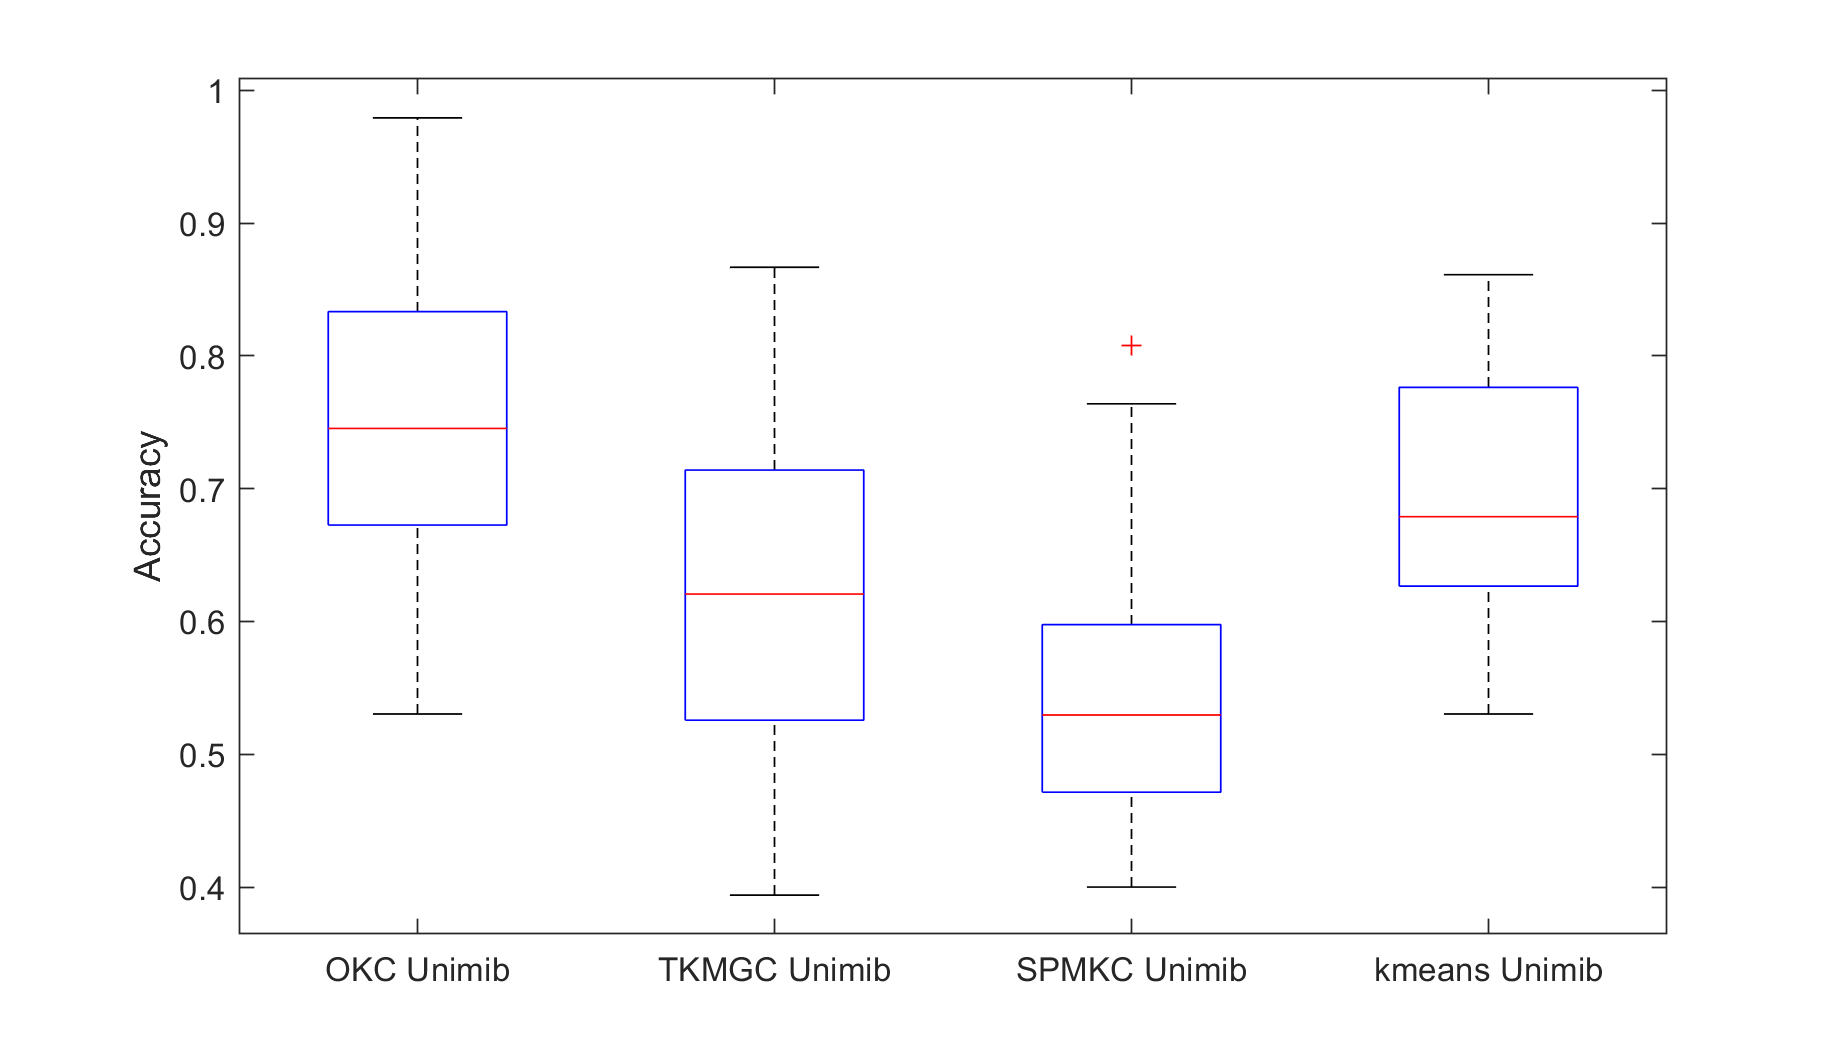
\includegraphics[scale=0.18]{boxplot_4_methods_0-100.png}
    \caption{Accuracy over 30 independent trials within interval $[0-100]$ on Unimib.}
    \label{Fig:9}
\end{figure}
Fig. \ref{Fig:10} shows that  the accuracy achieved by OKC within interval  $[101,200]$ is  higher than the one achieved within interval $[0,100]$ and still better than the performance achieved by TKMGC, SPMKC, and K-means.
\begin{figure}[htp]
    \centering
    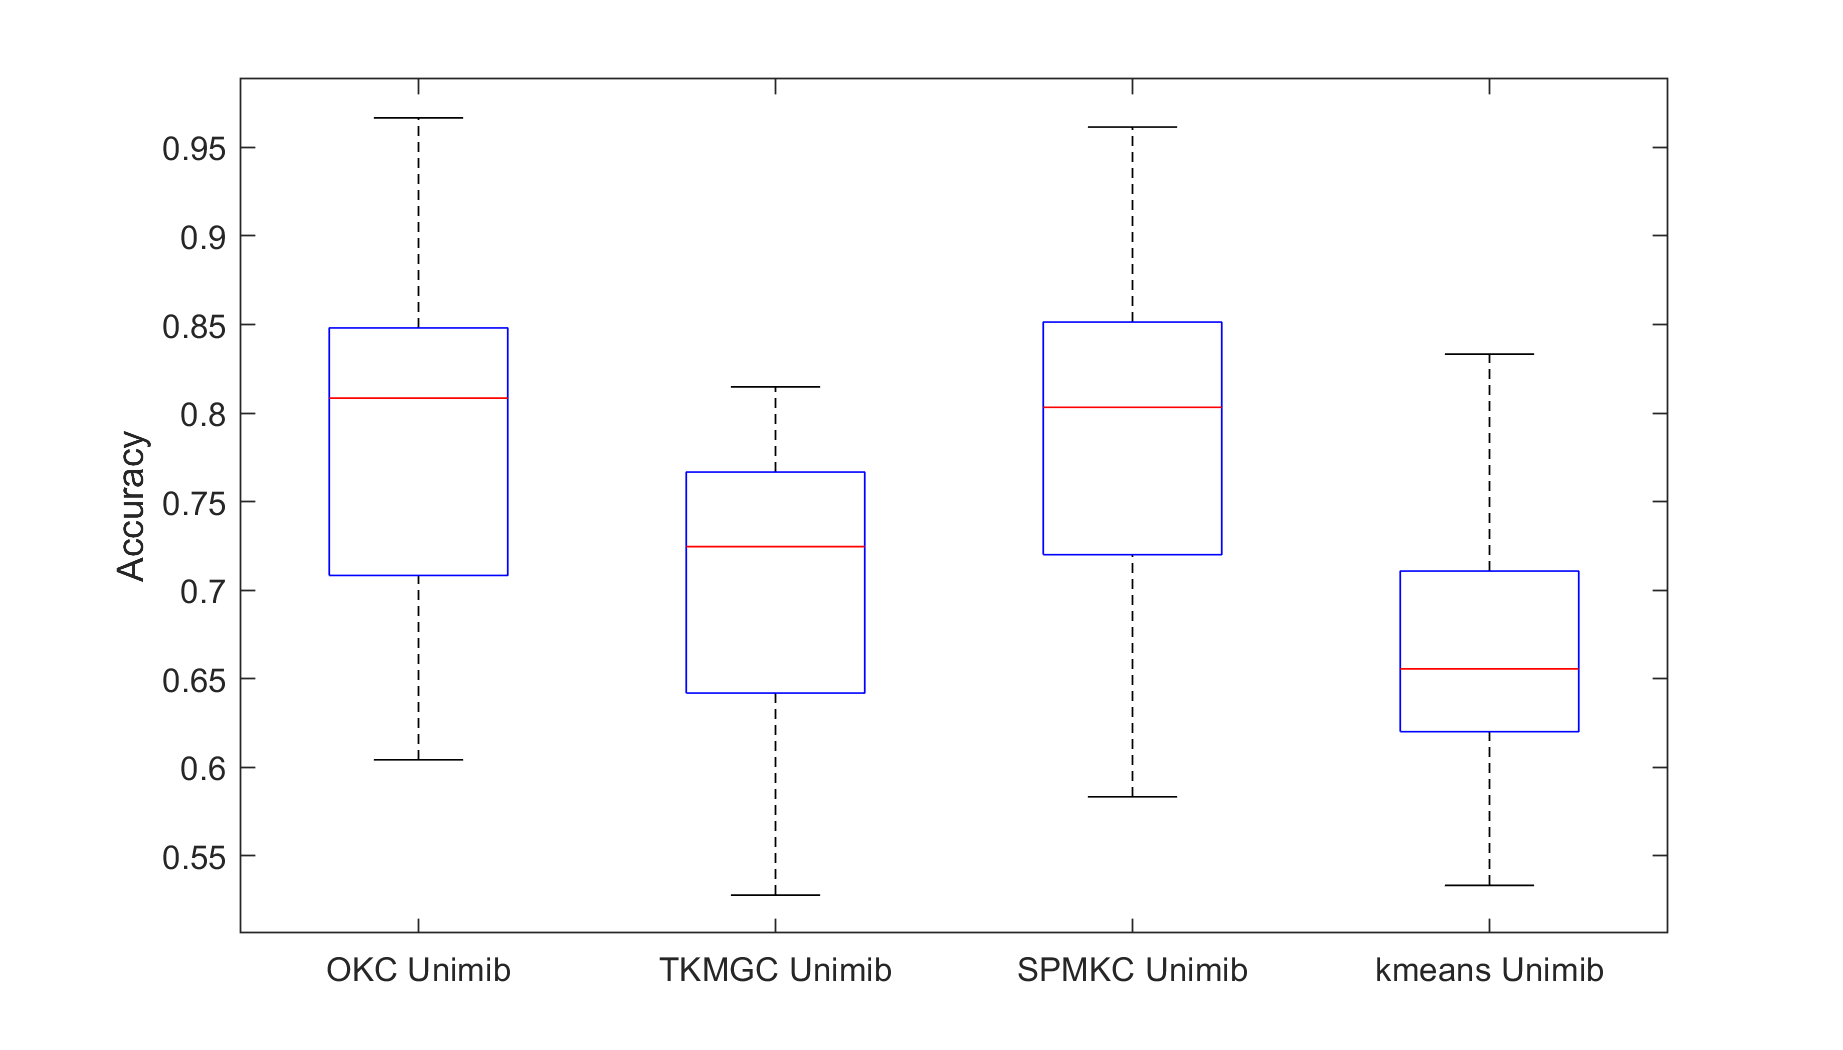
\includegraphics[scale=0.18]{boxplot_4_methods_101-200.png}
    \caption{Accuracy over 30 independent trials within interval $[101-200]$ on Unimib.}
    \label{Fig:10}
\end{figure}
Fig. \ref{Fig:11} depicts the accuracy within time interval $[201, 300]$. In this set of iterations, OKC achieves a slightly lower average accuracy of about $69\%$, but still outperforms the other algorithms, in terms of run time as well. Based on the results shown earlier, it can be inferred that the proposed scheme tends to achieve higher accuracy within $[101,200]$ which is when the 3rd class gets replaced with the 2nd class, thus reducing the number of classes from 3 to 2 within $[101,200]$. The same trend was observed with TKMGC and SPMKC. 
\begin{figure}[htp]
    \centering
    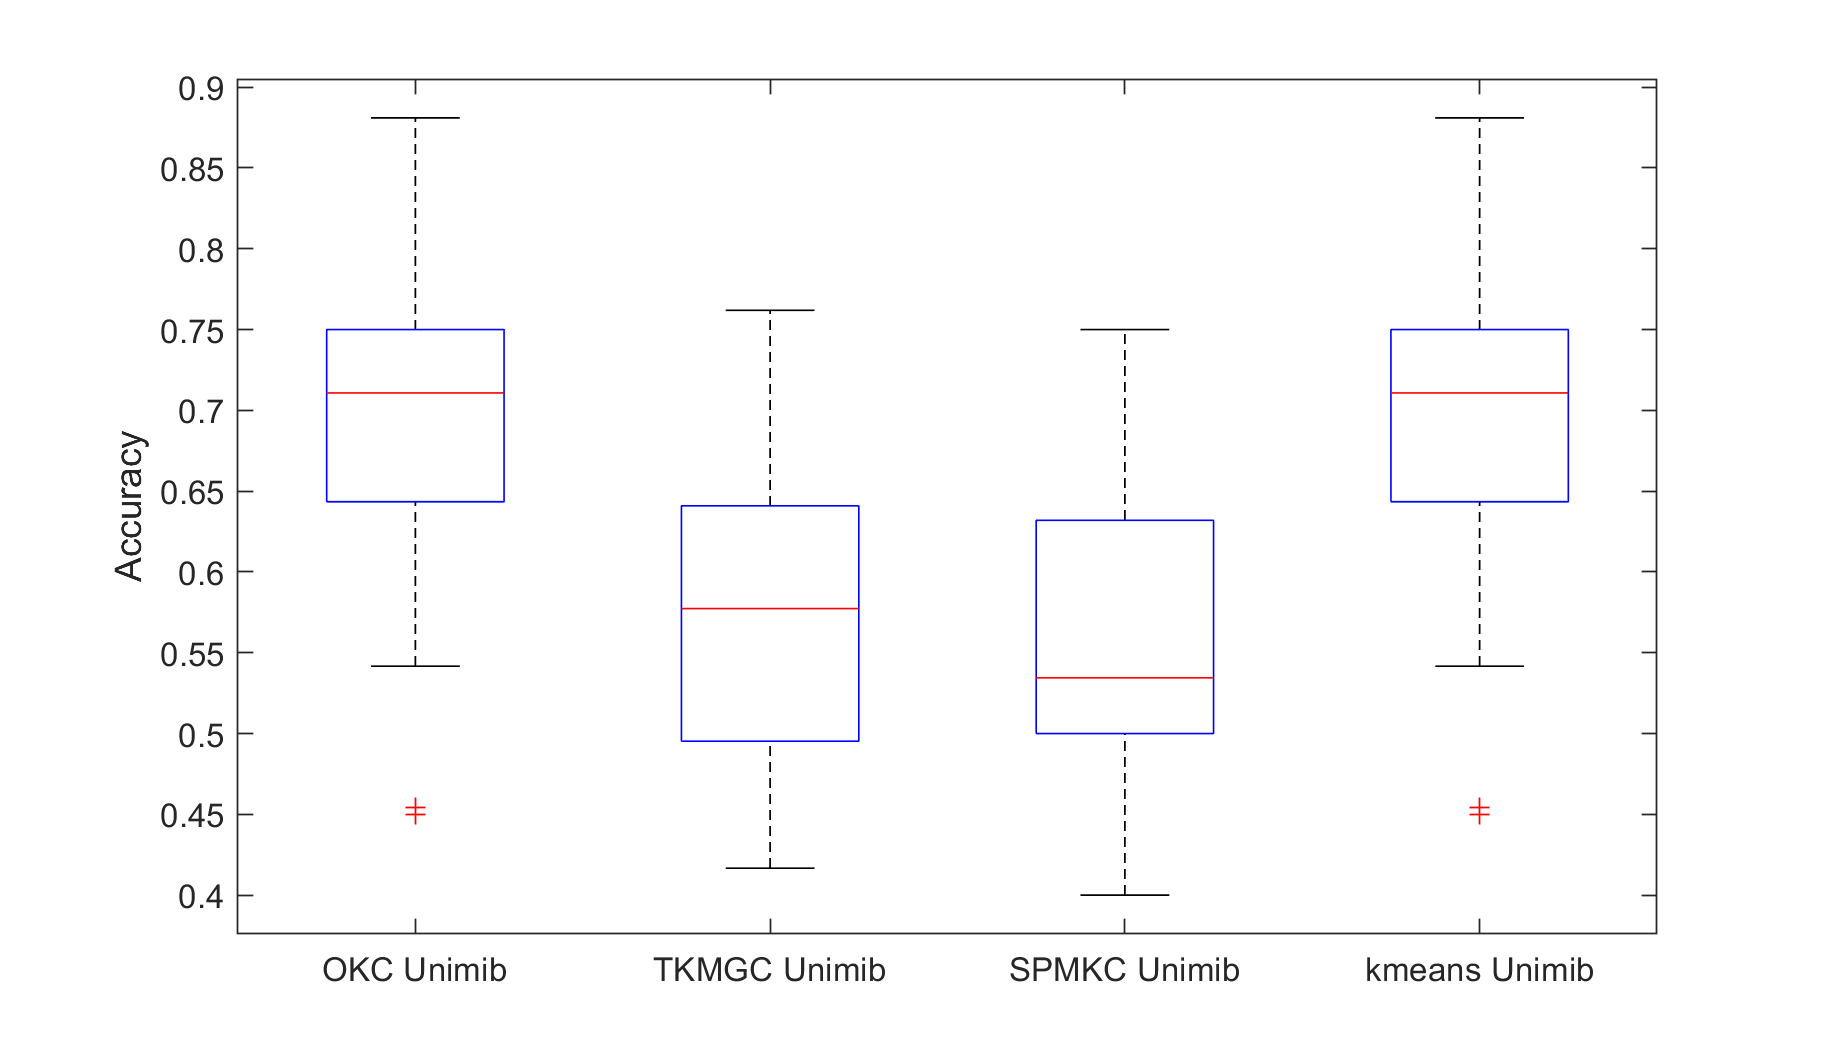
\includegraphics[scale=0.18]{boxplot_4_methods_201-300.png}
    \caption{Accuracy over 30 independent trials within interval $[201-300]$ on Unimib.}
    \label{Fig:11}
\end{figure}

Similarly, Figs. \ref{Fig:12}-\ref{Fig:14} depict the clustering accuracy on the  Salinas dataset over $100$ independent trials.OKC accuracy is a little bit over 90\% within the interval $[0,100]$. TKMGC achieves a slightly higher accuracy within $[0,100]$ though at the expense of a much higher average runtime  \textcolor{black}{TKMGC on Salinas exhibited the highest average runtime of about 593 seconds among all 100 experiments while OKC achieved almost similar average accuracy in just a fraction of TKMGC's runtime, i.e. in approximately 84 seconds.}. Moreover, SPMKC achieved an average accuracy of about 45\% and K-means roughly 81\% for average runtimes of approximately 125 seconds and 40 seconds, respectively.
\begin{figure}[htp]
    \centering
    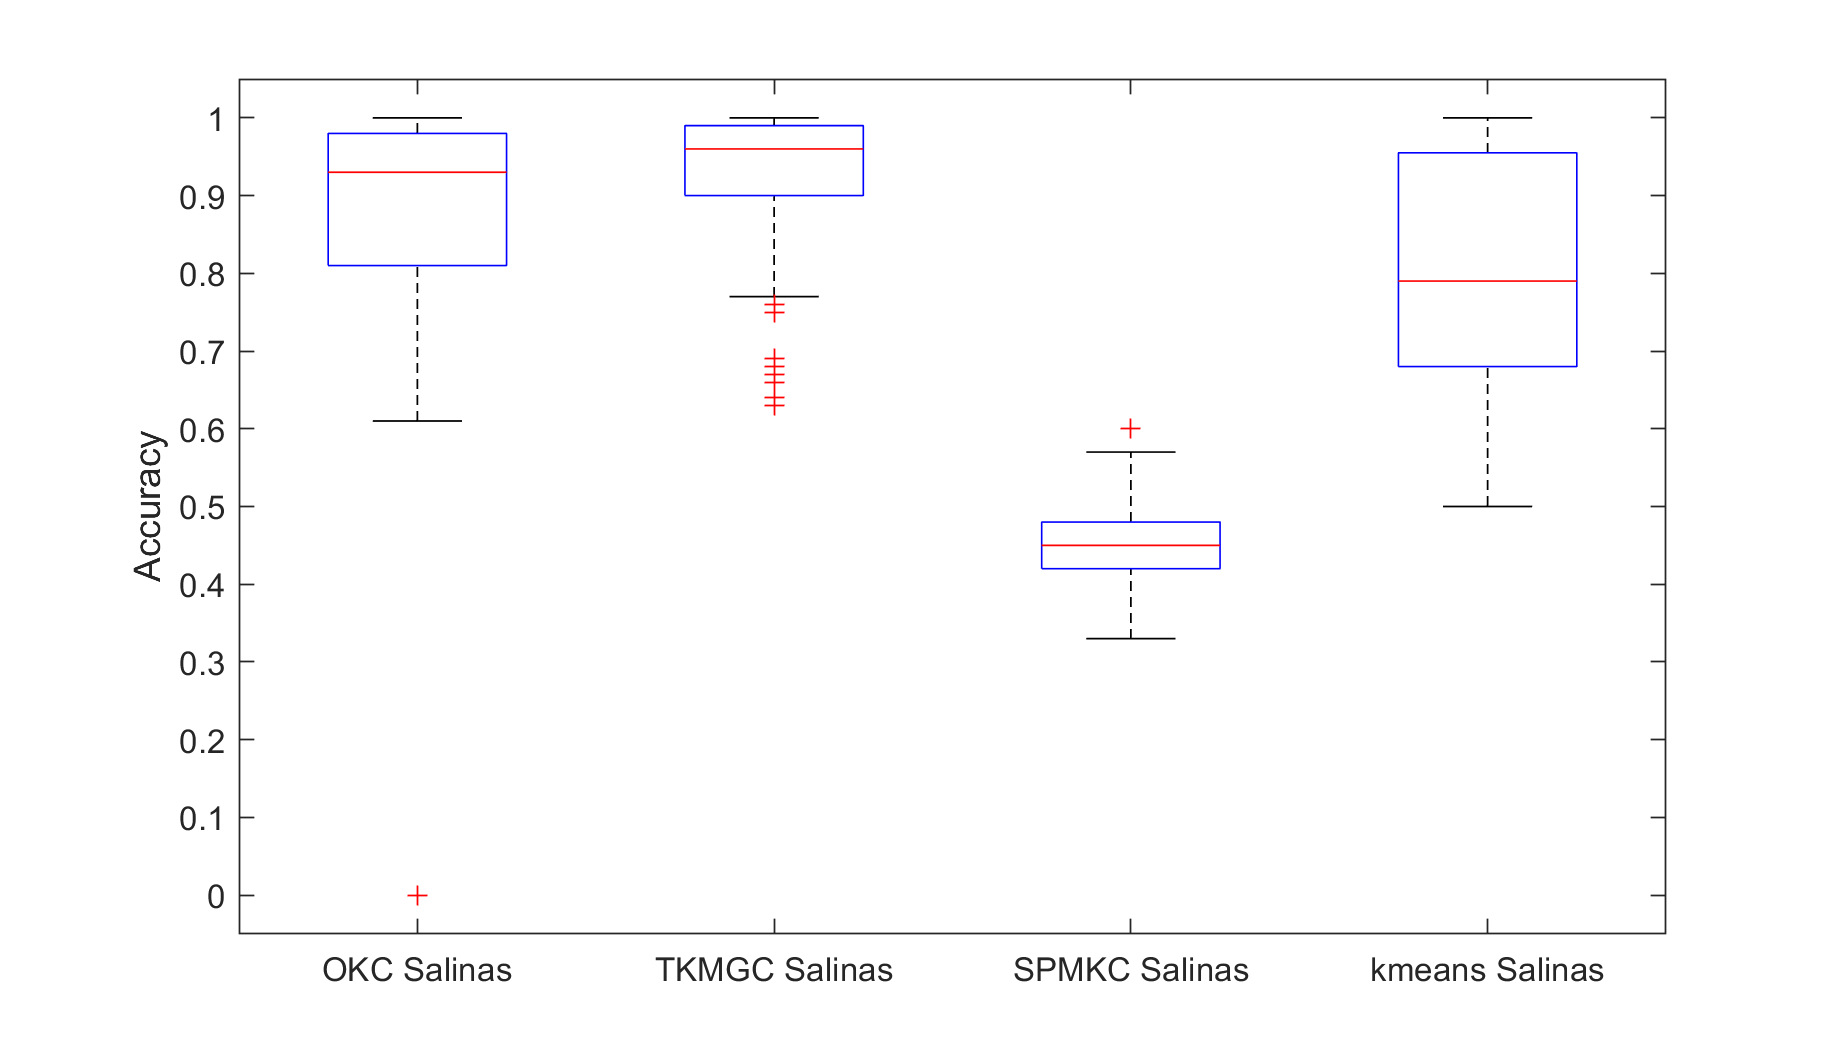
\includegraphics[scale=0.18]{boxplot_4_methods_Salinas_0-100.png}
    \caption{Accuracy over 30 independent trials within interval $[0-100]$ on Salinas.}
    \label{Fig:12}
\end{figure}
During interval $[101, 200]$ OKC outperformed all other three methods though the overall accuracy has decreased compared to interval $[0,100]$ which can attributed to the change in the number of classes while dealing with more classes compared to the Unimib dataset.
\begin{figure}[htp]
    \centering
    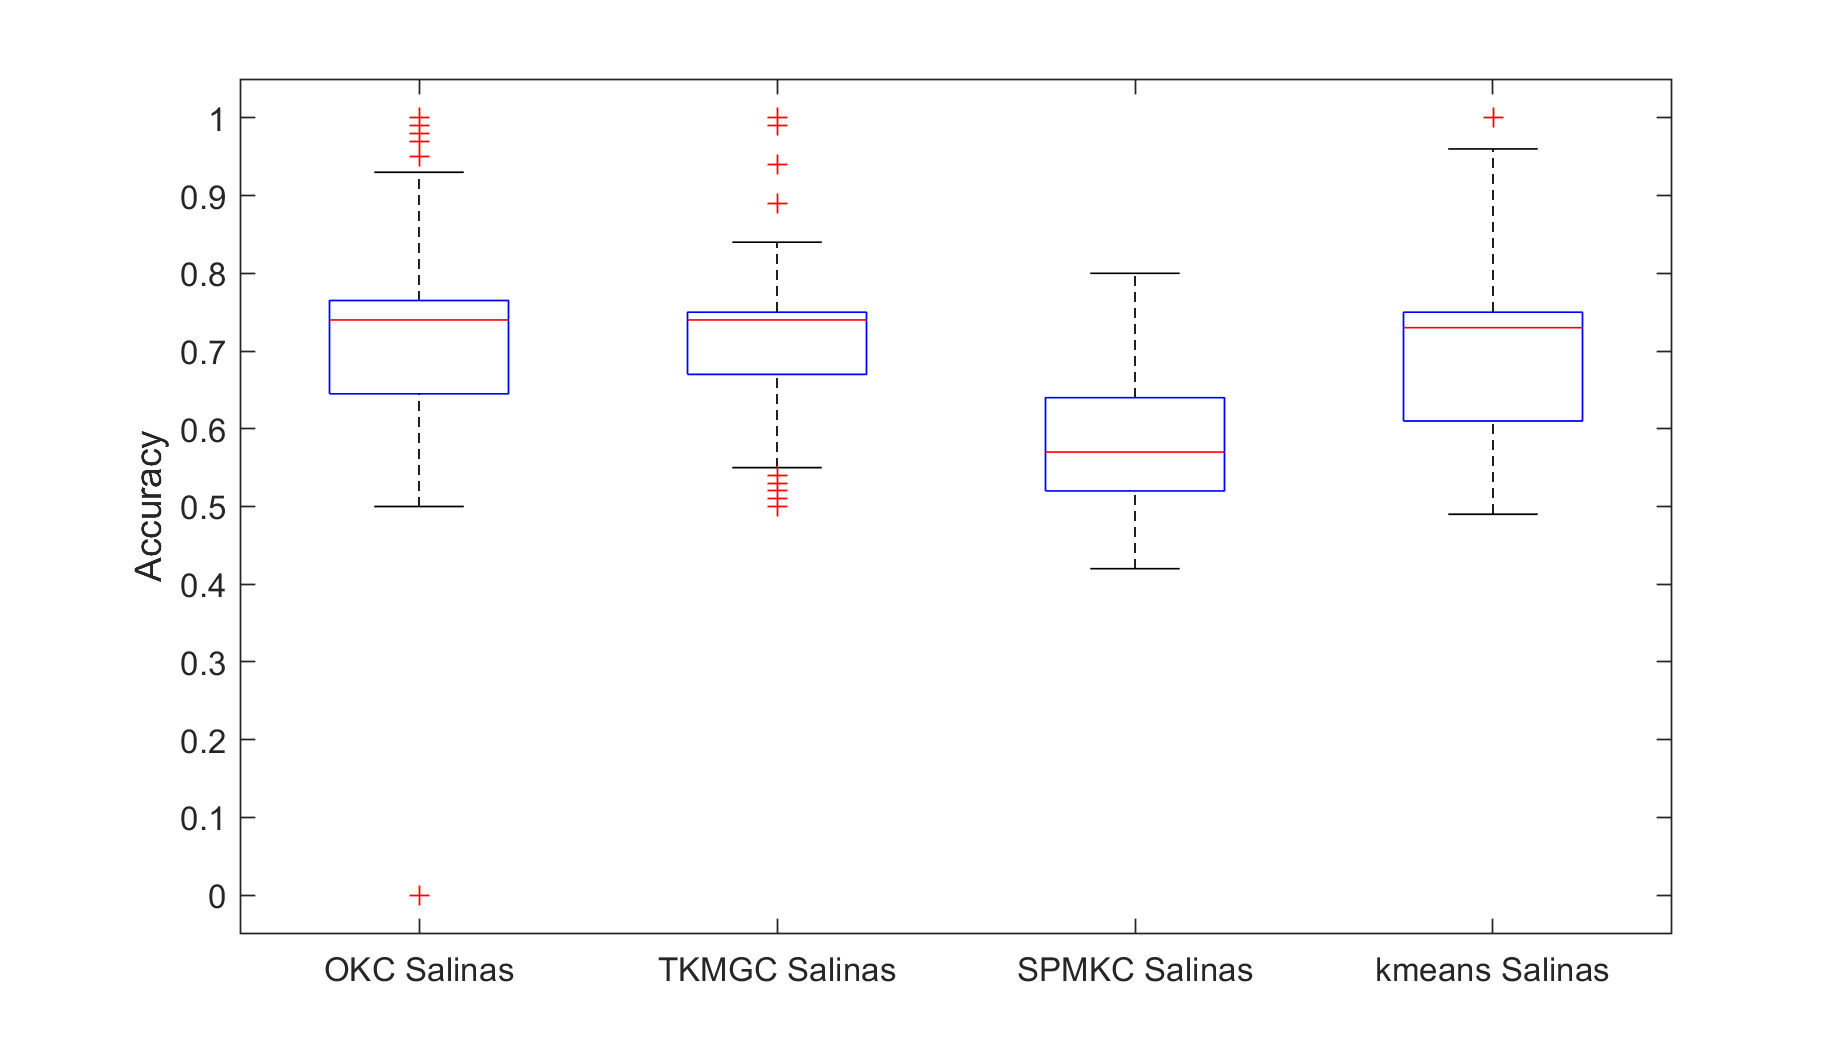
\includegraphics[scale=0.18]{boxplot_4_methods_Salinas_101-200.png}
    \caption{Accuracy over 30 independent trials within interval $[101-200]$ on Salinas.}
    \label{Fig:13}
\end{figure}
In Fig. \ref{Fig:14} OKC and TKMGC have almost identical accuracy though OKC offers way faster running time  as detailed earlier. Consequently, even in the last interval, the proposed method remains the most versatile algorithm among all the other tested schemes. 
\begin{figure}[htp]
    \centering
    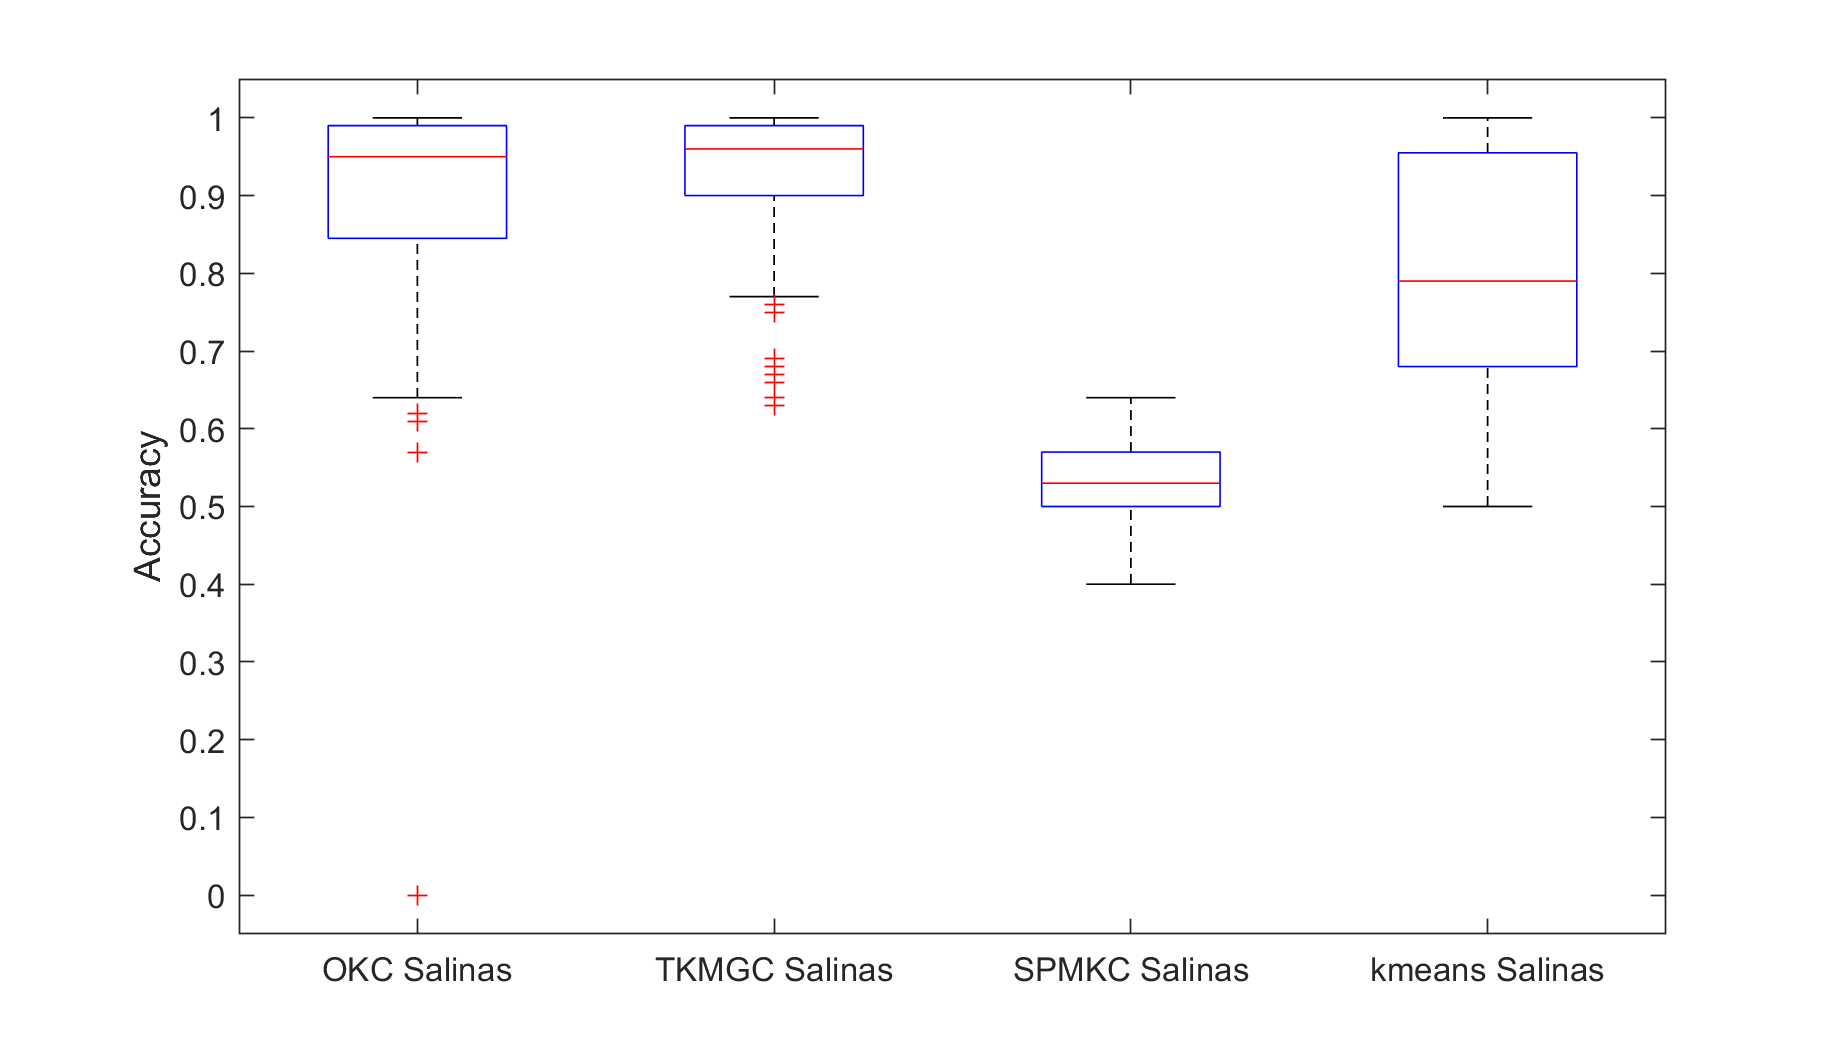
\includegraphics[scale=0.18]{boxplot_4_methods_Salinas_201-300.png}
    \caption{Accuracy over 30 independent trials within interval $[201-300]$ on Salinas.}
    \label{Fig:14}
\end{figure}

\section{Concluding Remarks}
A novel online joint kernel learning and clustering (OKC) framework has been derived which is capable of determining time-varying clustering configurations in an unsupervised manner. A novel time-dependent metric is devised to quantify online the closeness of candidate kernel similarity matrices to a block diagonal structure and facilitate clustering via sparse kernel matrix factorization. An effective interplay between block coordinate descent, difference of convex functions minimization and projected subgradient descent is devised to result an online iterative algorithm that updates online the kernel covariance matrix, as well as the associated clustering configuration. The resulting kernel iterates are proved to converge. Detailed numerical examples utilizing both synthetic and real data show the superior clustering accuracy achieved by OKC over existing alternatives while requiring considerably less running time.

\begin{thebibliography}{1}
\bibitem{Convex}
S. Boyd and L. Vandenberghe, \emph{Convex Optimization}. Cambridge University Press, 2004.

\bibitem{subgradient methods}
S. Boyd, L. Xiao, and A. Mutapcic, "Subgradient Methods". \emph{Notes for EE392O, Stanford University, Autumn 2003}.

%\bibitem{Sparsity Minimization}
%E.J. Candes, M.B. Wakin, and S.P. Boyd, "Enhancing Sparsity by Reweighted L1 Minimization". \emph{Journal of Fourier Analysis and Applications}, vol. 14, 877--905. 2008.

%\bibitem{NNMF for data representation}
%D. Cai, X. He, J. Han, T.S. Huang, "Graph Regularized Nonnegative Matrix Factorization for Data Representation," \emph{IEEE Transactions on Pattern Analysis and Machine Intelligence}, vol. 33, no. 8, 2011.

\bibitem{CCA}
J. Chen and I.D. Schizas. "Online Distributed Sparsity-Aware Canonical Correlation Analysis," \emph{IEEE Transactions on Signal Processing}, vol. 64, no. 3, 2016.

\bibitem{sensors}
J. Chen, A. Malhotra, and I.D. Schizas, "Data-Driven Sensors Clustering and Filtering for Communication Efficient Field Construction," \emph{Signal Processing}, 133, 155--168. 2017.

\bibitem{Simplex}
Y. Chen, X. Ye, "Projection Onto a Simplex," \emph{arXiv preprint arXiv:1101.6081}, 2011.

\bibitem{Kernel_Target}
N. Cristianini, J.S. Taylor, A. Elisseeff, and J. Kandola, "On Kernel-Target Alignment," \emph{Advances in Neural Information Processing Systems 14, MIT Press}, pp. 367--373, 2002.

\bibitem{Online Multiple Kernel Learning}
R. Ding, S.C.H. Hoi, and T. Yang, "Online Multiple Kernel Learning: Algorithms and Mistake Bounds,"{{\emph{International Conference on Algorithmic Learning Theory, Springer}, pp. 390--404, 2010.}}

\bibitem{OMKLGSF}
P.M. Ghari and Y. Shen. "Online Multi-Kernel Learning with Graph-Structured Feedback". \emph{Proceedings of Machine Learning Research}, vol.119, pg.3474-3483. 2020.

\bibitem{Salinas}
M. Grana, M.A. Veganzons, and B. Ayerdi. "Hyperspectral Remote Sensing Scenes," \emph{Available: https://www.ehu.eus/ccwintco/index.php/Hyperspectral
\_Remote\_Sensing\_Scenes\_Salinas}

\bibitem{Online MKL}
S.C.H. Hoi, R. Ding, P. Zhao, and T. Yang, "Online Multiple Kernel Classification," \emph{Machine Learning}, 90:289--316. 2013.

%\bibitem{NNMF Revisited}
%K. Huang, N.D. Sidiropoulos, and A. Swami, "Non-Negative Matrix Factorization Revisited: Uniqueness and Algorithm for Symmetric Decomposition", \emph{IEEE Transactions on Signal Processing}, vol. 62, no. 1, 2014.

\bibitem{Semi-supervised}
X.Y. Jing, F. Wu, X. Dong, S. Shan, and S. Chen, "Semi-Supervised Multi-view Correlation Feature Learning with Application to Webpage Classification". \emph{AAAI'17: Proceedings of the Third-First AAAI Conference on Artificial Intelligence}, pp. 1374--1381, Feb. 2017.

%\bibitem{Symmetric NMF}
%D. Kuang, C. Ding, and H. Park, "Symmetric Nonnegative Matrix Factorization for Graph Clustering,".\emph{Society for Industrial and Applied Mathematics. Proceedings of the SIAM International Conference on Data Mining}, 106--117, 2012.

\bibitem{Hungarian}
H. W. Kuhn, "The Hungarian Method for the Assignment Problem", \emph{Naval Research Logistics Quarterly}, no. 2, pg. 83--97, 1955.

\bibitem{LSOKL}
J. Lu, S.C.H. Hoi, J. Wang, P. Zhao, and Z.Y. Liu. "Large Scale Online Kernel Learning", \emph{Journal of Machine Learning Research}, vol.17, pg. 1-43. 2016.

%\bibitem{unconstrained minimization}
%M.J. Lai and J. Wang, "An Unconstrained lq Minimization with 0 < q < 1 for Sparse Solution of Undetermined Linear Systems," \emph{SIAM Journal on Optimization}, 21(1), 82--101, 2011.

\bibitem{Human_Activity}
A. Malhotra, I.D. Schizas, and V. Metsis, "Correlation Analysis-Based Classification of Human Activity Time Series," \emph{IEEE Sensors Journal}, vol. 18, no. 19,  2018.

%\bibitem{MILP}
%A. Malhotra and I.D. Schizas, "MILP-Based Unsupervised Clustering". \emph{IEEE Signal Processing Letters}, vol. 25, no. 12, July 2019.

\bibitem{DCA}
A. Malhotra and I.D. Schizas, "On Unsupervised Simultaneous Kernel Learning and Data Clustering,"{{\emph{Elsevier Pattern Recognition}, vol. 108, Dec. 2020.}}

\bibitem{Unimib}
D. Micucci, M. Mobilio, and P. Napoletano, "UniMib SHAR: A Dataset of Human Activity Recognition Using Acceleration Data from Smartphones," \emph{arXiv:1611.07688v5 [cs.CV]}, Aug. 2017.

\bibitem{MKL}
F. Orabona, L. Jie, and B. Caputo. "Multi Kernel Learning with Online Batch Optimization", \emph{Journal of Machine Learning Research}, vol.13, pg.227-253. 2012.

\bibitem{Neurocomputing}
F. Pompili, N. Gillis, P.A. Absil, and F. Glineur. "Two Algorithms for Orthogonal Nonnegative Matrix Factorization with Application to Clustering," \emph{Neurocomputing}, 141, pp. 15--25, 2014.

\bibitem{tkmgc}
Z. Ren, M. Mukherjee, M. Bennis, and J. Lloret, "Multikernel Clustering via Non-negative Matrix Factorization Tailored Graph Tensor Over Distributed Networks," \emph{IEEE Journal on Selected Areas in Communications}, vol. 39, no. 7,  2021.

\bibitem{SPMKC}
Z. Ren and Q. Sun, "Simultaneous Global and Local Graph Structure Preserving for Multiple Kernel Clustering," \emph{IEEE Transactions on Neural Networks and Learning Systems}, vol. 32, no. 5, 2021.

\bibitem{Distributed Informative-Sensor}
I.D.Schizas. "Distributed Informative-sensor Identification via Sparsity-Aware Matrix Decomposition". \emph{IEEE Transactions on Signal Processing}, vol. 61, no. 18, 2013.

\bibitem{Hyperspectral_Images}
K.T. Shahid and I.D. Schizas, ''Unsupervised Kernelized Correlation-Based Hyperspectral Unmixing with Mixing Pixels,'' \emph{IEEE Transactions on Geoscience and Remote Sensing}, vol. 57, no. 7, 2019.

\bibitem{OEML}
Y. Shen, T. Chen, and G.B. Giannakis. "Online-Ensemble Multi-kernel Learning Adaptive Non-stationary and Adversarial Environments", \emph{Proceedings of Machine Learning Research}, vol.84. 2018.

\bibitem{Random OMKL}
Y. Shen, T. Chen, and G.B. Giannakis. "Random Feature-based Online Multi-kernel Learning in Environments with Unknown Dynamics", \emph{Journal of Machine Learning Research}, vol.20, pg. 1-36. 2019.

\bibitem{Convex Analysis}
P.D. Tao and L.T.H. An, "Convex Analysis Approach to DC Programming: Theory Algorithms and Applications," \emph{Acta Mathematica Vietnamica}, vol. 22, no. 1, pp. 289--355, 1997.

%\bibitem{Deep Matrix Factorization}
%G. Trigeorgis, K. Boumalis, S. Zafeiriou, and B.W.Schuller, "A Deep Matrix Factorization Method for Learning Attribute Representations," \emph{IEEE Transactions on Pattern Analysis and Machine Intelligence}, vol. 39, no. 3, 2017.

%\bibitem{Maximum Margin Clustering}
%H. Valizadegan and R. Jin, "Generalized Maximum Margin Clustering and Unsupervised Kernel Learning," \emph{Advances in Neural Information Processing Systems}, pp. 1417--1424, 2007.

\bibitem{NNMF Comprehensive}
Y.X. Wang and Y.J. Zhang, "Nonnegative Matrix Factorization: A Comprehensive Review," \emph{IEEE Transactions on Knowledge and Data Engineering}, vol. 25, no. 6, 2013.

%\bibitem{Minimization of l1-l2}
%P. Yin, Y. Lou, Q. He, and J. Xin, "Minimization of l1-l2 for Compressed Sensing," \emph{SIAM Journal on Scientific Computing}, 37(1), A536--A563, 2015.

%
\end{thebibliography} 

%\appendices

\section{Appendix}
%\newline
\noindent \textbf{A. Proof of Lemma \ref{Lemma:Metric}}\label{Apdx:A}\newline
The first term in $B_t(\cdot)$ in \eqref{eq:Nonstationary} is nonnegative by definition. From linear algebra it holds that $\|\bbv\|_{1}\geq \|\bbv\|_2$ therefore the second and third terms in the sum in \eqref{eq:Nonstationary} are also nonnegative. Thus, the metric $B_t(\cdot)\geq 0$.

If $\bbK_t(\bbx_{\tau})=\sum_{b=1}^B\alpha_b\bbK^b_{\tau}(\bbx_{\tau})$ is constructed with kernel coefficients such that it is block diagonal with rank equal to $Q$, then $\|\bbK_t(\bbx_{\tau})-\bbW\bbY^T\|_{F}^2=0$. Further, being block diagonal implies that each row of $\bbW$ and $\bbY$ can have at most one nonzero entry. Thus, 
$\|\bbW_{\ell,:}\|_1=\|\bbW_{\ell,:}\|_2$ and $\|\bbY_{\ell,:}\|_1=\|\bbY_{\ell,:}\|_2$ for $\ell=1,\ldots,P$. Thus, a block diagonal kernel mapping of rank $Q$ will make the metric $B_t(\cdot)=0$. Thus, it can be utilized to measure how close to a block diagonal structure $\bbK_t(\bbx_{t})$ is at time instant $t$. \myQED

\noindent\textbf{B. Subgradient Derivations}\label{Apdx:B}

%\subsection{Proof of the Corollary 1}\label{A:Dlesn}
%Original objective/cost function:
%\begin{eqnarray}\label{eq_eqn}
%\sum_{t=0}^{\tau}\beta^{t-\tau}||\sum_{j=1}^{B}\alpha_jK_j-\mathbf{XY}^T||_F^2+v(\sum_{i=1}^{P}||\mathbf{X_i,:}||_1-||\mathbf{X_i,:}||_2)\\
%+v(||\mathbf{Y_i,:}||_1-||\mathbf{Y_i,:||_2})+\mu(\sum_{i=1}^{Q-1}\lambda_q(\sum_{j=1}^{B}\alpha_jK_j)\nonumber\\
%-\sum_{i=1}^{Q}\lambda_q(\sum_{j=1}^{B}\alpha_jK_j))\nonumber
%\end{eqnarray}
%s.t. \begin{math}X\geq0,Y\geq0,\alpha_j\geq0,\alpha_j\geq0,\sum_{j=1}^{B}\alpha_j=1\end{math}

%Hence, G(x) and H(x) can be expressed as:
%\begin{eqnarray}\label{eq_eqn}
%\mathbf{G(x)} = \sum_{t=0}^{\tau}\beta^{t-\tau}||\sum_{j=1}^{B}\mathbf{\alpha_jK_j}-\mathbf{WY}^T||_F^2+v(\sum_{i=1}^{P}||\mathbf{W_i,:}||_1\\
%+||\mathbf{Y_i,:}||_1)+\mu(\sum_{i=1}^{Q-1}\lambda_q(\sum_{j=1}^{B}\mathbf{\alpha_jK_j))}\nonumber
%\end{eqnarray}
%\begin{eqnarray}\label{eq_eqn}
%\mathbf{H(x)} = v(-||\mathbf{W_i,:}||_2-||\mathbf{Y_i,:||_2})-\mu(\sum_{i=1}^{Q}\lambda_q(\sum_{j=1}^{B}\mathbf{\alpha_jK_j}))
%\end{eqnarray}
%Subgradient in terms of X:
%\begin{eqnarray}\label{eq_eqn}
%\mathbf{\delta H}(\mathbf{W},\mathbf{Y},\mathbf{\alpha_j}) = \frac{-3\mathbf{W_P_Q}}{\sqrt{\mathbf{W_1_1}^2+\mathbf{W_1_2}^2+...+\mathbf{W_P_Q}^2}}
%\end{eqnarray}
%Subgradient in terms of Y:
%\begin{eqnarray}\label{eq_eqn}
%\mathbf{\delta H}(\mathbf{W},\mathbf{Y},\mathbf{\alpha_j}) = \frac{-3\mathbf{Y_P_Q}}{\sqrt{\mathbf{Y_1_1}^2+\mathbf{Y_1_2}^2+...+\mathbf{Y_P_Q}^2}}
%\end{eqnarray}
%Subgradient in terms of alpha:
%\begin{eqnarray}\label{eq_eqn}
%\mathbf{\delta H}(\mathbf{W},\mathbf{Y},\mathbf{\alpha}_j) = [\mathbf{\alpha}_j^k]_Q
%\end{eqnarray}
%where,
%\begin{eqnarray}\label{eq_eqn}
%[\mathbf{\alpha}_j^k]_Q = \begin{bmatrix}\mathbf{\mu}_1^k'\mathbf{K}^1\mathbf{\mu}_1^k+\mathbf{\mu}_2^k'\mathbf{K}^2\mathbf{\mu}_2^k+...+\mathbf{\mu}_Q^k'\mathbf{K}^1\mathbf{\mu}_Q^k\\
%\mathbf{\mu}_1^k'\mathbf{K}^2\mathbf{\mu}_1^k+\mathbf{\mu}_2^k'\mathbf{K}^2\mathbf{\mu}_2^k+...+\mathbf{\mu}_Q^k'\mathbf{K}^2\mathbf{\mu}_Q^k\\
%.............................................................\\
%\mathbf{\mu}_1^k'\mathbf{K}^B\mathbf{\mu}_1^k+\mathbf{\mu}_2^k'\mathbf{K}^B\mathbf{\mu}_2^k+...+\mathbf{\mu}_Q^k'\mathbf{K}^B\mathbf{\mu}_Q^k\end{bmatrix}
%\end{eqnarray}
%Therefore, at k = 0, X and \begin{math}\alpha_b\end{math} updates while Y remains constant:
%\begin{eqnarray}\label{eq_eqn}
%\mathbf{min} \sum_{t=0}^{\tau}\beta^{t-\tau}||\sum_{j=1}^{B}\mathbf{\alpha}_j\mathbf{K}_j-\mathbf{WY}^T||_F^2+v(\sum_{i=1}^{P}||\mathbf{W_i,:}||_1)\\
%+\mu(\sum_{i=1}^{Q-1}\lambda_q(\sum_{j=1}^{B}\mathbf{\alpha}_j\mathbf{K}_j))-(\mathbf{\delta H}(\mathbf{W},\mathbf{Y},\mathbf{\alpha}_j)^T\*\mathbf{W})\nonumber\\
%-([\mathbf{\alpha}_j^k]_Q^T\*\alpha_b)\nonumber
%\end{eqnarray}
%and k = 1, Y updates while both X and \begin{math}\alpha_b\end{math} remain constant:
%\begin{eqnarray}\label{eq_eqn}
%\mathbf{min} \sum_{t=0}^{\tau}\beta^{t-\tau}||\sum_{j=1}^{B}\mathbf{\alpha}_j\mathbf{K}_j-\mathbf{WY}^T||_F^2+v(\sum_{i=1}^{P}||\mathbf{Y_i,:}||_1)\\
%-(\mathbf{\delta H}(\mathbf{W},\mathbf{Y},\mathbf{\alpha}_j)^T\*\mathbf{Y})\nonumber
%\end{eqnarray}
%Alternatively, (9) can be expressed as:
%\begin{eqnarray}\label{eq_eqn}
%\mathbf{min} \sum_{t=0}^{\tau}\beta^{t-\tau}||\sum_{j=1}^{B}\mathbf{\alpha}_j\mathbf{K}_j-\mathbf{WY}^T||_F^2+v(\sum_{i=1}^{P}||\mathbf{W_i,:}||_1)\\
%+\mu(\sum_{i=1}^{Q-1}\lambda_q(\sum_{j=1}^{B}\mathbf{\alpha}_j\mathbf{K}_j)) - v(\sum_{i=1}^{P}<\delta||\mathbf{W}_i,:||_2,||\mathbf{W}_i,:||_1>)\nonumber\\
%-\mu([\mathbf{\alpha}_j^k]_Q)^T\mathbf{\alpha}_b\nonumber
%\end{eqnarray}
The first term in the cost in (17) can be rewritten as 
\begin{align}\label{eq:Cost_first_term_details}
&\sum_{\tau=0}^{t}\beta^{t-\tau}||\sum_{b=1}^{B}\mathbf{\alpha}_b\mathbf{K}_{\tau}^b(\bbx_{\tau})-\mathbf{W}\hat{\bbY}_{t,\kappa}^T||_F^2=\\
&=\sum_{\tau=0}^{t}\beta^{t-\tau}\textrm{tr}(\sum_{b=1}^{B}\mathbf{\alpha}_{b}\mathbf{K}_{\tau}^{b}(\bbx_{\tau})-\mathbf{W}\hat{\bbY}_{t,\kappa}^T)\nonumber\\
&\times(\sum_{b'=1}^{B}\mathbf{\alpha}_{b'}\mathbf{K}_{\tau}^{b'}(\bbx_{\tau})-\mathbf{W}\hat{\bbY}_{t,\kappa}^T)^T\nonumber\\
&=\sum_{\tau=0}^{t}\beta^{t-\tau}\sum_{b=1}^{B}\sum_{b'=1}^{B}\mathbf{\alpha}_b\mathbf{\alpha}_{b'}^T\mathbf{tr}(\mathbf{K}_{\tau}^{b}(\bbx_{\tau})\cdot\mathbf{K}_{\tau}^{b'}(\bbx_{\tau}))\nonumber\\
&-2\sum_{\tau=0}^{t}\beta^{t-\tau}\sum_{b=1}^{B}\mathbf{\alpha}_b\mathbf{tr}(\mathbf{K}_{\tau}^{b}(\bbx_{\tau})\hat{\bbY}_{t,\kappa}\mathbf{W}^T)\nonumber\\
&+\sum_{\tau=0}^{t}\beta^{t-\tau}\mathbf{tr}(\mathbf{W}\hat{\bbY}_{t,\kappa}^T\hat{\bbY}_{t,\kappa}\mathbf{W}^T)\nonumber
\end{align}
which can be rewritten as:
\begin{align}\label{eq:Cost_first_term_details_b}
&\sum_{\tau=0}^{t}\beta^{t-\tau}{\bbalpha}^T\bbG_{\tau}{\bbalpha}\nonumber\\
&-2\sum_{\tau=0}^{t}\beta^{t-\tau}{\bbalpha}^T\bbg_{\tau}^{t,\kappa}+\sum_{t=0}^{\tau}\beta^{t-\tau}\mathbf{tr}(\mathbf{W}\hat{\bbY}_{t,\kappa}^T\hat{\bbY}_{t,\kappa}\mathbf{W}^T),
\end{align}
where the structure of matrices $\bbG_{\tau}$ and $\bbg_{\tau}^{t,\kappa}$ is given in \eqref{eq:G_and_g}.

Calculating the subgradient  for each term of the cost in  (17) with respect to factor $\bbW$ results the following (if term is differentiable subgradient coincides with gradient). The first term in (17) [expanded in \eqref{eq:Cost_first_term_details}] is differentiable with respect to $\bbW$ resulting
%%
\begin{align}\label{eq:First_term}
2\sum_{\tau=0}^{t}\beta^{t-\tau}(\bbW\hat{\bbY}_{t,\kappa}^T-\sum_{b=1}^{B}\alpha_{b}\mathbf{K}_{\tau}^b(\bbx_{\tau}))\hat{\bbY}_{t,\kappa}
\end{align}
%%
the second and fourth terms in (17) have subgradients
%%
\begin{align}\label{eq:Sec_term}
& v*\textrm{sgn}({\bbW}),\\
& \bbdelta_{\bbW} J_{t,\kappa,\rho}=
\left[\frac{\bbW_{1,:,t,\kappa,\rho}^T}{||\mathbf{W}_{1,:,t,\kappa,\rho}||_2^{-1}},\ldots,
\frac{\bbW_{P,:,t,\kappa,\rho}^T}{||{\bbW}_{P,:,t,\kappa,\rho}||_2^{-1}}
\right]^T.
\end{align}
%%
Similarly, the gradient of the first term in (17) [or \eqref{eq:Cost_first_term_details}] w.r.t $\bbalpha$ is 
%%
\begin{equation}
 2\sum_{\tau=0}^{t}\beta^{t-\tau}[\mathbf{G}_{\tau}\bbalpha-\bbg_{\tau}^{t,\kappa}]
\end{equation}
%%
whereas the subgradients of third and fifth terms in (17) are 
$[\bbdelta\bbalpha]_{Q-1,t,\kappa,\rho}$ and $\bbdelta_{\bbalpha} J_{t,\kappa,\rho}$ detailed in \eqref{eq:Subgradient_Formulas_alpha} and \eqref{eq:DCA_Subgrads}.
Thus, justifying the (sub)-gradients given in \eqref{eq:Sub_F_t_W}.

In the same way we can determine the (sub)-gradients of the cost in (24) w.r.t factor $\bbY$. In detail, the first term of (24) can be written similarly as in 
\eqref{eq:Cost_first_term_details_b} which when differentiated w.r.t $\bbY$ gives
%%
\begin{align}\label{eq:Sub_F_t_W_2}
 2\sum_{\tau=0}^{t}\beta^{t-\tau}({\bbY}\hat{\bbW}_{t,\kappa+1}^T-\sum_{b=1}^{B}\alpha_{b}^{t,\kappa+1}\mathbf{K}_{\tau}^b(\bbx_{\tau})))\hat{\bbW}_{t,\kappa+1}.
 \end{align}
 The subgradient of the second and third terms in (24) is 
 %%
\begin{align}\label{eq:Sec_term}
& v*\textrm{sgn}({\bbY}),\\
& \bbdelta_{\bbY}\ J_{t,\kappa,\rho}=
\left[\frac{\bbY_{1,:,t,\kappa,\rho}^T}{||\mathbf{Y}_{1,:,t,\kappa,\rho}||_2^{-1}},\ldots,
\frac{\bbY_{P,:,t,\kappa,\rho}^T}{||{\bbY}_{P,:,t,\kappa,\rho}||_2^{-1}}
\right]^T.
\end{align}
%%
 Thus, justifying the (sub)-gradient given in \eqref{eq:Sub_F_t_Y}.\myQED

\textbf{C. Proof of Proposition 1}\label{thm:Central_Conv}\newline
%We start with the inner most loops in Alg. 1 that minimize the convex costs involved in \eqref{eq:Majorized_F_Walpha} and 	\eqref{eq:Majorized_F_Y}, in steps a.2 and b.2, via projected subgradient-descent.
Since the subgradients associated with \eqref{eq:Majorized_F_Walpha} and 	\eqref{eq:Majorized_F_Y} are bounded for dictionary kernels $\bbK_{\tau}^b(\bbx_{\tau})$ with finite eigenvalues, and since a diminishing step-size rule $\frac{c}{\phi}$ is utilized that is square-summable but not summable then according to the convergence results in \cite[pg. 4-5]{subgradient methods}
the updates $\hat{\bbW}_{t,\kappa,\rho+1}^{\phi}$ and 
$\hat{\bbalpha}_{t,\kappa,\rho+1}^{\phi}$ converge as $\phi\rightarrow\infty$ to the optimal solution of \eqref{eq:Majorized_F_Walpha}, namely $\hat{\bbW}_{t,\kappa,\rho+1},\hat{\bbalpha}_{t,\kappa,\rho+1}$. Similarly, updates $\hat{\bbY}_{t,\kappa,\rho+1}^{\phi}$ converge to the optimal solution of 
\eqref{eq:Majorized_F_Y}, namely $\hat{\bbY}_{t,\kappa,\rho+1}$, as $\phi\rightarrow\infty$.

Utilizing Thm 3. in \cite{Convex Analysis}, it turns out that Steps a.1 and a.2 of Alg. 1  applied to minimize  cost function $F_t(\bbW,\bbalpha)$ in \eqref{eq:DC_Walpha} for fixed $\bbY=\hat{\bbY}_{\tau,\kappa}$,  
result a decreasing sequence of cost values, i.e., for $\rho=0,1,\ldots$
%%
\begin{align}\label{eq:Decr_1}
F_t(\hat{\bbW}_{t,\kappa,\rho+1},\hat{\bbalpha}_{t,\kappa,\rho+1}) \leq 
F_t(\hat{\bbW}_{t,\kappa,\rho},\hat{\bbalpha}_{t,\kappa,\rho}). 
\end{align}
%%

Similarly, Steps b.1 and b.2 of Alg. 1  applied to minimize  cost function $F_t(\bbY)$ in \eqref{eq:DC_Y} for fixed $\bbW=\hat{\bbW}_{\tau,\kappa+1}, \bbalpha=\hat{\bbalpha}_{\tau,\kappa+1}$,  result a decreasing sequence of cost values, i.e., for $\rho=0,1,\ldots$
%%
\begin{align}\label{eq:Decr_2}
F_t(\hat{\bbY}_{t,\kappa,\rho+1}) \leq 
F_t(\hat{\bbY}_{t,\kappa,\rho}). 
\end{align}
%%

Recall that $\hat{\bbW}_{t,\kappa+1}=\hat{\bbW}_{t,\kappa,R}$, $\hat{\bbalpha}_{t,\kappa+1}=\hat{\bbalpha}_{t,\kappa,R}$, and  $\hat{\bbY}_{t,\kappa+1}=\hat{\bbY}_{t,\kappa,R}$. 
Also, $F_t(\bbW,\bbalpha)=F_t(\bbW,\bbalpha,\hat{\bbY}_{t,\kappa})$ in \eqref{eq:DC_Walpha}, and 
and $F_t(\bbY)=F_t(\hat{\bbW}_{t,\kappa+1},\bbalpha_{t,\kappa+1},{\bbY})$ in \eqref{eq:DC_Y} with $F_t(\bbW,\bbY,\bbalpha)$ denoting the cost function in \eqref{eq:Eq1}.
Therefore from \eqref{eq:Decr_2} we have
%%
\begin{align}\label{eq:Cost_Reduct_1}
    &F_t(\hat{\bbW}_{t,\kappa+1},\hat{\bbalpha}_{t,\kappa+1},\hat{\bbY}_{t,\kappa+1})=F_t(\hat{\bbY}_{t,\kappa+1})=F_t(\hat{\bbY}_{t,\kappa,R}) \nonumber\\
    &\leq F_t(\hat{\bbY}_{t,\kappa})=F_t(\hat{\bbW}_{t,\kappa+1},\hat{\bbalpha}_{t,\kappa+1},\hat{{\bbY}}_{t,\kappa})
\end{align}
%%
Notice that  from \eqref{eq:Decr_1} we obtain
%%
\begin{align}\label{eq:Cost_Reduct_2}
 & F_t(\hat{\bbW}_{t,\kappa+1},\hat{\bbalpha}_{t,\kappa+1},\hat{{\bbY}}_{t,\kappa})=F_t(\hat{\bbW}_{t,\kappa+1},\hat{\bbalpha}_{t,\kappa+1})\nonumber\\
  &=F_t(\hat{\bbW}_{t,\kappa,R},\hat{\bbalpha}_{t,\kappa,R})
  \leq F_t(\hat{\bbW}_{t,\kappa,0},\hat{\bbalpha}_{t,\kappa,0})
  %F_t(\hat{\bbW}_{t,\kappa},\hat{\bbalpha}_{t,\kappa},\hat{{\bbY}}_{t,\kappa}),
\end{align}
%%
and $F_t(\hat{\bbW}_{t,\kappa,0},\hat{\bbalpha}_{t,\kappa,0})=
  F_t(\hat{\bbW}_{t,\kappa},\hat{\bbalpha}_{t,\kappa},\hat{{\bbY}}_{t,\kappa}).$
Thus, from \eqref{eq:Cost_Reduct_1} and \eqref{eq:Cost_Reduct_2} we obtain
that the iterates $\hat{\bbW}_{t,\kappa+1},\hat{\bbalpha}_{t,\kappa+1},\hat{{\bbY}}_{t,\kappa}$ lead to a decreasing cost sequence $F_t$ during time instant $t$, i.e.,
%%
\begin{align}\label{eq:Cost_reduction}
F_t(\hat{\bbW}_{t,\kappa+1},\hat{\bbalpha}_{t,\kappa+1},\hat{\bbY}_{t,\kappa+1})\leq F_t(\hat{\bbW}_{t,\kappa},\hat{\bbalpha}_{t,\kappa},\hat{{\bbY}}_{t,\kappa}).
\end{align}
%%
The cost function $F_t$ in \eqref{eq:Eq1} is bounded from below from quantity $-\lambda_{Q}(\sum_b\alpha_b\bbK_{t}^b(\bbx_{\tau}))$ which is finite for finite-entry dictionary kernel matrices in ${\cal D}_t$. Thus, from \eqref{eq:Cost_reduction} and the monotone convergence theorem it follows
%%
\begin{equation}\label{eq:Lim_1}
\textrm{lim}_{\kappa\rightarrow\infty}F_t (\hat{\bbW}_{t,\kappa},\hat{\bbalpha}_{t,\kappa},\hat{{\bbY}}_{t,\kappa})=f_{t},
\end{equation}
where $f_{t}$ is a finite valued converging point.

Thus, given the continuity of cost function $F_t$ the iterates 
$\hat{\bbW}_{t,\kappa},\hat{\bbalpha}_{t,\kappa},\hat{{\bbY}}_{t,\kappa}$ also converge as $k\rightarrow\infty$ for each time  $t$.
\myQED




\end{document}



